%% stevensthesis_num.tex
%% Copyright 2008 B. E. Arnett
%
% ----->  Latex is not required for writing your dissertation or thesis.  Most theses in liberal arts and other areas are done in Word or WYSIWYG editors
%------>  Latex is frequently used in math, physics and computer science for ease in producing formulas.
%------>  This template is provided for Latex users to help in the formatting of the thesis or dissertation.
%------>  This work is not maintained by Stevens Library anymore and is provided on an: "as is" basis.
%
% This work may be distributed and/or modified under the conditions of the LaTeX Project Public License, either version 1.3 of this license or (at your option) any later version.
% The latest version of this license is in http://www.latex-project.org/lppl.txt and version 1.3 or later is part of all distributions of LaTeX version 2005/12/01 or later.
%
% This work has the LPPL maintenance status `maintained'.
%
%
% This work consists of the files stevensthesis_num.tex and the derived file pgnumchapter_nums.sty.

%
% This file may serve as a template for dissertation / thesis submission for Stevens Institute of Technology.
%
% There are fields in titlepg.sty that must be updated with your own information.  The file pgnumchapter.sty must be included but  does not need to be updated, unless you want to change the layout of your pages and chapters.
%
% Both dissertations and master thesis can be created from this program.
% These fields should be changed:
%    {thesistype} should be either "dissertation" or "thesis"
%    {thesisdegree} should be either "doctor of philosophy" for dissertation or
%            "Master of Engineering - Electrical Engineering"
%            "Master of Science - Computer Science"   or the correct degree designation.
%
%
% Please see the formatting instructions on the library website at
%      https://library.stevens.edu/services/submit-theses-dissertations/dissertation-submission
%
% This file was adapted for the DRIFT thesis. The preamble, packaging and page-numbering
% machinery below is unmodified from the Stevens template; only the front-matter body
% below \begin{document} and the chapter/appendix \include list were changed to point at
% the DRIFT chapter files and to remove the doctoral-only Vita section. See
% paper/THESIS_TEMPLATE_SETUP.md in the DRIFT repository for the full list of changes.

\documentclass[12pt]{report}
\usepackage {fancyhdr}
\usepackage{graphicx, amssymb, changepage}
\usepackage{rotating}
\usepackage{setspace}
\usepackage{pgnumchapter_nums}
\usepackage{titlepg}
\usepackage{multirow} % multi row in tables
\usepackage{float}% for table and figure enforce placement, the [H] option
\usepackage{titlesec}% more layers of sections
\usepackage{bbm} %bold in math
\usepackage{subfig}% subfigs
\usepackage{array}%include tables with first row bold
\newcolumntype{@}{>{\global\let\currentrowstyle\relax}}
\newcolumntype{^}{>{\currentrowstyle}}
\newcommand{\rowstyle}[1]{\gdef\currentrowstyle{#1}%
  #1\ignorespaces
}
\usepackage{threeparttable}%table with notes
  %table/figure move left
\usepackage{changepage}
  %table cmidrule
\usepackage{booktabs}
\usepackage{longtable} % lets a table break across a page instead of running off the bottom margin

%include algorithm/flow charts
\usepackage[noend]{algorithmic}
\usepackage{algorithm}
% \usepackage{algpseudocode}
\newcommand{\LINEFORALL}[2]{%
    \STATE\algorithmicforall\ {#1}\ \algorithmicdo\ {#2} %
}
\renewcommand{\algorithmiccomment}[1]{\bgroup\hfill//~#1\egroup}

% colors for reviews
% color conflict with xthesis fixed by this: https://tex.stackexchange.com/questions/119486/another-issue-with-universitys-class-file-and-tikz-package-relates-to-queens
\usepackage{color}
\usepackage[usenames,dvipsnames]{xcolor}
\newcommand{\ion}[1]{{\bf {\textcolor{WildStrawberry}{IF:  #1}}}}
\newcommand{\luis}[1]{{\bf {\textcolor{BurntOrange}{HZ:  #1}}}}
% plotting
\usepackage{tikz}
\usetikzlibrary{matrix}
% roman letters
\newcommand{\rom}[1]{\expandafter{\romannumeral #1}}
\newcommand{\RNum}[1]{\uppercase\expandafter{\romannumeral #1\relax}}
% interesting symbols
\usepackage{pifont}
% differential d
\newcommand{\de}{\text{\rm d}}
% add appendix
\usepackage[toc,page]{appendix}
% use natbib
\usepackage{natbib}
% hyperlink reference
% colorlinks=true + pdfborder={0 0 0} so cross-references print as plain
% colored text rather than with a visible box drawn around every \ref/\cite,
% which is hyperref's default and looks wrong in a printed or PDF-viewed thesis.
\RequirePackage[citecolor=blue,urlcolor=blue,linkcolor=black,colorlinks=true,pdfborder={0 0 0}]{hyperref}
% THEOREMS ----------------------------------------------------------------
\usepackage{amsthm,amsmath,amsfonts,newlfont}
\theoremstyle{plain}
\newtheorem{thm}{Theorem}[section]
\newtheorem{cor}[thm]{Corollary}
\newtheorem{lem}[thm]{Lemma}
\newtheorem{prop}[thm]{Proposition}
\newtheorem{prob}[thm]{Problem}
\newtheorem{ques}[thm]{Question}
\newtheorem{ass}[thm]{Assumption}
\def\proof{{\bf{Proof.}}}
%
\theoremstyle{definition}
\newtheorem{defn}{Definition}[section]
%
\theoremstyle{remark}
\newtheorem{rem}{Remark}[section]
\newtheorem{example}{Example}[section]
%
\numberwithin{equation}{section}
\renewcommand{\theequation}{\thesection.\arabic{equation}}
%%% -----------------------------------------------------------------------

%              this is for the list of symbols page, if desired
\def\listofsymbols{\input{symbols} \clearpage}
\def\addsymbol #1: #2#3{$#1$\> \parbox{5in}{#2 \dotfill  \pageref{#3}}\\}
\def\newnot#1{\label{#1}}
%
\pagestyle{fancy}
% \fancyhead[LE,RO]{helv \thepage}
\fancyhead[L,R]{helv \thepage}
\setlength{\headheight}{15.2pt}     %%test this

%\fancyhead[LE,RO]{\thepage\hspace{2em}\footnotesize{\leftmark}}  % try this to move over header

\addtolength{\voffset}{-4em}   								% May2009 added this to move page number up a bit

\doublespacing

\lhead{}
\chead{}
\rhead{\thepage}
\lfoot{}
\cfoot{}
\rfoot{}

\renewcommand{\headrulewidth}{0 pt}          %this prints a line under the header
\renewcommand{\footrulewidth}{0  pt}            %this prints a line under the footer

\renewcommand{\contentsname}{\normalsize{Table of Contents}}
\renewcommand{\listfigurename}{\normalsize{List of Figures}}
\renewcommand{\listtablename}{\normalsize{List of Tables}}
\renewcommand{\bibname}{\normalsize{Bibliography}}
\renewcommand{\indexname}{\normalsize{Index}}

% bea02152011 - commented out the following line.  This line reformats the table of contents subsection appearance,
% to look like n.nn (chapterNumber dot sectionNumber subsectionNumber)instead of
% n.n.n  (chapterNumber dot sectionNumber dot subsectionNumber )
%   \renewcommand{\thesubsection}{\thesection\arabic{subsection}}

% you may need to change the pdfpagewidth to pagewidth
% and pdfpageheight to pageheight

% if not using pdflatex to produce output, you may need to change to pagewidth and pageheight variables.
%\pagewidth 8.5in
%\pageheight 11in
\pdfpagewidth 8.5in
\pdfpageheight 11in
%

\setlength{\oddsidemargin}{0.5in}
\setlength{\evensidemargin}{0.5in}
\setlength{\textwidth}{6.0in}
\setlength{\textheight}{8.5in}
\setlength{\topmargin}{0.in}
\setlength{\headheight}{0.5in}
\setlength{\headwidth}{6.0in}
\setlength{\headsep}{0.65in}                       			% change from .25in to .5 in   May2009
\setlength{\parindent}{12mm}

%%%%%%%%%%%%%%%%%%%%%%%%%%%%%%%%%%%%%%%%%%%
%
% If you only want to create output that includes only certain chapters
%
%\includeonly{chapter2}
%%%%%%%%%%%%%%%%%%%%%%%%%%%%%%%%%%%%%%%%%%%

%%%%%%%%%%%%%%%%%%%%%%%%%%%%%%%%%%%%%%%%%%%%
%%%
%%%  This begins the frontmatter of the document, everything preceding the body
%%%
%%%%%%%%%%%%%%%%%%%%%%%%%%%%%%%%%%%%%%%%%%%%

\begin{document}

\pagenumbering{roman}

\thesistitlepage

\thesiscopyrightpage

\addcontentsline{toc}{chapter}{Abstract}          		 				% added May2009
\thesisabstract

% Dedication page omitted by request.

\addcontentsline{toc}{chapter}{Acknowledgments}   				% added May2009
\thesisacknowledgments

\makeatletter \renewcommand{\@dotsep}{10000} \makeatother

\renewcommand{\contentsname}{\normalsize{Table of Contents}}      % added this line May2010 to fix issue with
\tableofcontents                                                 %toc appearing in too large a font size when used in Linux

\newpage		% added June 2009

\addcontentsline{toc}{chapter}{List of Tables}     					% added May2009
\listoftables

\newpage     % added June2009
\addcontentsline{toc}{chapter}{List of Figures}						% added May2009
\listoffigures

%%%%%%%%%%%%%%%%%%%%%%%%%%%%%%%%%%%%%%%%%%%%
%%%
%%%  This begins the body of the document
%%%
%%%%%%%%%%%%%%%%%%%%%%%%%%%%%%%%%%%%%%%%%%%%

\newpage
\pagenumbering{arabic}

% Each chapter is a separate file, listed in thesis order. Adding, removing, or
% reordering a chapter is a matter of editing this list; nothing else in this
% file needs to change.
%
% While drafting a single chapter, uncomment the line below and list only the
% chapter(s) you are working on. This skips typesetting the other ~90 pages,
% which is the single biggest lever against Overleaf's free-plan compile
% timeout. Comment it back out (or delete it) before a full, final compile.
%\includeonly{chapter5}
\chapter{Introduction}
\label{chap:introduction}

\section{The Problem}
\label{sec:the-problem}

Consider an assistant that is told ``I live in Boston'' and, three months later, ``I moved to Seattle.'' Both statements enter the agent's memory. Both are semantically close to the query ``where do I live.'' A retrieval function that ranks by similarity and recency will often return the older fact alongside the newer one, and the language model that composes the answer has no reliable signal telling it which of the two candidates is still true. The result is an agent that answers from a fact whose validity has already ended.

This is not a retrieval failure in the conventional sense. The correct fact was stored, and it could be found by the retrieval function precisely because it remained similar to the query. The failure is one of memory hygiene: nothing in the system marks the older fact as no longer current, and nothing removes it once a newer fact supersedes it.

The failure compounds with time. An agent that operates for a year accumulates thousands of facts, an increasing fraction of which have been superseded by later observations. Every superseded fact that is retrieved is context spent on misinformation rather than on the true state of the world, and every superseded fact that reaches the answer model is an opportunity to produce a confidently wrong statement about something the user has already corrected. As language model agents move from single-session tools toward assistants that persist across months of interaction, the volume of stale material in memory grows in proportion to the agent's own lifetime, and the cost of ignoring it grows with it.

\section{Why the Problem Has Not Been Settled}
\label{sec:why-not-settled}

Production memory systems for language model agents address the storage and retrieval halves of this problem well. MemGPT organizes an agent's context as a paged hierarchy, treating the active context window as physical memory and an external store as disk \citep{packer2023memgpt}. Zep builds a temporal knowledge graph purpose-built for agent memory \citep{rasmussen2025zep}. Mem0 provides a scalable long-term store aimed at production deployment \citep{chhikara2025mem0}. A-MEM organizes memory agentically, with a language model deciding how memories should be structured and linked \citep{xu2025amem}. In each of these systems, the treatment of information that has been superseded by later observations is secondary to the treatment of storage and retrieval, and where a forgetting mechanism exists at all, its design is chosen by the system's authors rather than measured against alternatives.

The reason this gap persists is partly methodological rather than a simple oversight. Comparing forgetting rules across published systems is confounded: the systems under comparison differ simultaneously in their substrate, their retrieval function, their extraction pipeline, their prompting, and often their underlying language model. When one system is observed to handle a stale-fact scenario better than another, the difference cannot be cleanly attributed to the forgetting rule, because four other variables changed at the same time. What is missing from the literature is not another memory architecture. It is a controlled comparison in which the forgetting policy is the only variable that changes.

This thesis supplies that comparison. The framework built to run it, called DRIFT, holds the memory substrate, the fact extraction step, the retrieval function, the answer-generating model, and the evaluation judge fixed across every experimental condition, and varies only the rule that decides what memory keeps, discards, or hides at answer time.

\section{Hypothesis}
\label{sec:hypothesis}

The central hypothesis of this thesis is stated as follows.

\begin{quote}
\textbf{H.} Selective forgetting grounded in bitemporal structure improves an agent's answer quality and cost profile relative to both append-only memory and to structure-blind or novelty-based forgetting.
\end{quote}

Bitemporal structure, defined precisely in Chapter~\ref{chap:method}, means that each stored fact carries two independent timelines: the interval during which the fact was true of the world, and the interval during which the agent believed it. A forgetting policy grounded in this structure can distinguish a fact that has been explicitly superseded by a later observation from a fact that is merely old, which is the distinction that a policy based on age alone, or on textual novelty alone, cannot make.

\section{Research Questions}
\label{sec:research-questions}

The hypothesis is decomposed into four research questions, each answered with evidence in Chapter~\ref{chap:results}.

\begin{description}
\item[RQ1.] Does append-only memory, the default behavior of most deployed systems, measurably surface superseded facts at answer time?
\item[RQ2.] Among the candidate forgetting policies, which offers the best trade-off between accuracy, staleness, and computational cost?
\item[RQ3.] Does bitemporal structure specifically outperform structure-blind alternatives, or is any graph-aware consolidation strategy sufficient to obtain the same benefit?
\item[RQ4.] Do the policy rankings established under single-agent use survive multi-agent use, in which the agent that reads a fact is not necessarily the agent that wrote it?
\end{description}

\section{Novelty}
\label{sec:novelty}

The contribution of this thesis is not a new memory architecture. Bitemporal modeling has a decades-long history in database research, and Zep has already applied a form of it to agent memory \citep{rasmussen2025zep}. The novelty here is experimental and lies in what a properly controlled design makes visible that an uncontrolled comparison cannot.

\paragraph{N1: The forgetting policy isolated as an independent variable.} To the best of the author's knowledge, this is the first study that holds the substrate, the extraction step, the retrieval function, the answer model, and the judge fixed, and varies only the forgetting rule, across a taxonomy spanning no memory, append-only retention, time-based decay, contradiction-based invalidation, novelty gating, language-model consolidation, and topology-based consolidation. Published comparisons between memory systems confound the forgetting rule with several other design choices simultaneously, which makes it impossible to attribute an observed difference in behavior to the forgetting rule alone.

\paragraph{N2: The bitemporal-versus-structure-blind ablation.} One policy in the taxonomy, referred to throughout this thesis as P5, is constructed for a single purpose: it is structure-aware, it operates on the same knowledge graph as the winning policy, it performs the same category of consolidation, and it is deliberately denied access to valid time, so that it must resolve competing facts by structural corroboration instead of by temporal currency. This design isolates the contribution of bitemporal semantics from the contribution of graph structure in general. Without this ablation, a result showing that a bitemporal policy beats a naive baseline would be equally consistent with the more generic explanation that graph-aware reasoning of any kind helps, and would say nothing specific about temporality. With the ablation in place, the claim becomes specific, and on real-world knowledge updates it becomes decisive, as Chapter~\ref{chap:results} reports.

\paragraph{N3: Novelty gating identified and measured as a failure mode.} Write-side novelty gating, in which a candidate fact is rejected before it is ever stored because it is judged too similar to something already in memory, is currently promoted in the literature as an efficiency technique \citep{wang2026sage}. This thesis gives the first controlled demonstration that on any workload in which facts get corrected over time, a novelty gate trades a bounded saving in memory footprint for an unbounded liability in correctness, and demonstrates the mechanism directly from saved knowledge-graph snapshots rather than by argument alone.

\paragraph{N4: A negative result about the standard benchmarks.} The two most widely used benchmarks for agent memory, LoCoMo and LongMemEval, carry zero annotations of the superseded answer for any of their questions, and therefore cannot support any measurement of whether an agent has correctly revised a belief \citep{maharana2024locomo,wu2025longmemeval}. Identifying this gap, and identifying two benchmarks that close it, is itself a contribution to how this subfield evaluates memory revision.

Two further methodological findings emerged while reconciling experimental runs against one another rather than being planned in advance: a configuration ablation that separates the contribution of the policy itself from the contribution of a domain-specific configuration choice, and a judge-reliability audit that quantifies how much of a reported result can be attributed to noise in the evaluation procedure rather than to the policy under test. Both are reported in full in Chapter~\ref{chap:results}.

\section{Contributions}
\label{sec:contributions}

This thesis makes the following contributions.

\begin{enumerate}
\item A controlled experimental framework in which the forgetting policy is the only independent variable over a fixed substrate, retrieval function, extraction step, answer model, and judge, described in Chapter~\ref{chap:method}.
\item A staleness metric kept separate from accuracy, together with the finding that the two most widely used agent-memory benchmarks cannot support it, and the identification of two benchmarks that can, described in Chapter~\ref{chap:experimental-setup}.
\item Replicated evidence, on two benchmarks of different provenance, that bitemporal invalidation is free of accuracy cost, that novelty gating causes unrecoverable staleness, and that time-blind consolidation is significantly worse than bitemporal consolidation, described in Chapter~\ref{chap:results}.
\item An equivalence result rather than merely a null result. Paired bootstrap intervals bound the accuracy difference between bitemporal invalidation and the append-only ceiling to within roughly two and a half points on both benchmarks, which is a materially stronger claim than a failure to reject a null hypothesis.
\item A configuration ablation separating the contribution of the forgetting policy from the contribution of a domain declaration that the policy depends on.
\item A judge-reliability audit that establishes a noise floor for language-model-judged accuracy under a rotating pool of evaluator models, and that identifies a specific twelve-and-a-half-point artifact traced to that rotation.
\item An open, dependency-free software implementation that runs its entire test suite offline in a fraction of a second and integrates into a third-party agent in five lines of code, described in Appendix~\ref{app:reproduction}.
\end{enumerate}

\section{Organization of the Thesis}
\label{sec:organization}

Chapter~\ref{chap:related-work} situates DRIFT among existing agent memory systems, consolidation research, write-side control techniques, and staleness-focused benchmarks. Chapter~\ref{chap:method} describes the bitemporal substrate, the experimental pipeline, the seven policies under comparison, the metrics reported, and the statistical procedures used to test them. Chapter~\ref{chap:experimental-setup} describes the benchmark selection process, including the negative result concerning the standard benchmarks, the two benchmarks ultimately used, the models involved, and the reproducibility infrastructure. Chapter~\ref{chap:results} reports the experimental results in full, organized around the four research questions, together with the configuration ablation and the judge-reliability audit. Chapter~\ref{chap:discussion} discusses why the results take the shape they do, considers the impact of the work for research and for practice, states the threats to the validity of the conclusions in full, and closes with the limitations of the study and its conclusion. Appendix~\ref{app:results} contains the complete per-cell results and the full pairwise significance matrix. Appendix~\ref{app:reproduction} contains the figure index, the dataset schema, the exact commands needed to reproduce every reported number, and a short example of integrating DRIFT into a third-party agent.
   % Introduction
\chapter{Related Work}
\label{chap:related-work}

This chapter situates DRIFT among four bodies of work: production memory systems for language model agents, research on the risks of memory consolidation, write-side control techniques for what enters memory in the first place, and benchmarks that treat staleness as a first-class evaluation target rather than an afterthought. Each section closes by stating precisely what the cited work does not do, which is the gap this thesis addresses.

\section{Agent Memory Systems}
\label{sec:related-memory-systems}

The last several years have produced a series of memory architectures aimed at extending a language model agent's effective context beyond what fits in a single prompt.

MemGPT introduced an operating-system-inspired design in which the agent's context window is treated as physical memory and an external store is treated as disk, with the model itself issuing function calls to page information in and out \citep{packer2023memgpt}. This design is primarily concerned with the mechanics of what enters and leaves the active context at a given moment, and it does not distinguish between information that is merely old and information that has been superseded by a later observation.

Zep constructs a temporal knowledge graph specifically for agent memory and is the closest architectural relative of the substrate used in this thesis \citep{rasmussen2025zep}. Zep records the interval during which a fact was valid, which is the same primitive DRIFT's substrate relies on. What Zep's published work does not do is compare alternative policies for acting on that temporal information: it demonstrates that recording validity intervals is useful for retrieval quality, but it does not ask which of several possible rules for using those intervals to forget, invalidate, or retain facts performs best, nor does it report a staleness metric distinct from answer accuracy. This is precisely the comparison DRIFT is built to run, using a similar temporal primitive as its starting point.

Mem0 targets production deployment with a scalable long-term memory store, emphasizing operational concerns such as latency and storage cost at scale \citep{chhikara2025mem0}. A-MEM organizes memory agentically, delegating decisions about memory structure and linking to a language model rather than fixing them in advance \citep{xu2025amem}.

All four systems are systems contributions: each proposes an architecture and demonstrates that the architecture improves some measure of retrieval quality or operational efficiency relative to a simpler baseline. None of the four isolates the forgetting rule as a variable that can be swapped while everything else about the system is held constant, and none reports an accuracy metric alongside a metric that specifically measures whether the agent's answer reflects a fact that has already been superseded. Comparing them to one another, or to any single one of them, cannot answer the question this thesis asks, because in each comparison the forgetting rule changes together with the substrate, the retrieval function, and often the underlying model.

\section{Consolidation and Its Risks}
\label{sec:related-consolidation}

A separate line of work treats memory consolidation, the periodic act of rewriting, summarizing, or pruning stored memories, as a technique that can degrade an agent's behavior rather than only improve it. Zhang et al. show that memories consolidated through repeated language-model rewriting degrade in quality over time, to the point where an agent's task utility can fall below what the same agent would achieve with no memory at all \citep{zhang2026faulty}. Their headline finding, that a capable model fails on the majority of a set of previously solved reasoning problems once its memory of the solutions has been consolidated by repeated rewriting, is a direct warning against treating consolidation as a strictly beneficial operation. This finding motivates one of the design decisions of this thesis: rather than assuming that language-model consolidation is an improvement, DRIFT treats it as a policy under test, on equal footing with every other candidate. It appears in the taxonomy of Chapter~\ref{chap:method} as policy P4, evaluated with the same metrics and the same statistical rigor applied to every other policy, rather than assumed to be a baseline improvement.

\section{Write-Side Control}
\label{sec:related-write-side}

A third line of work intervenes earlier in the pipeline, at the point where a candidate fact is either admitted to memory or rejected before it is ever stored. Wang et al. propose SAGE, which uses a von Mises-Fisher density estimator over memory embeddings to classify an incoming fact as clearly novel, clearly redundant, or uncertain, routing clearly novel facts directly into memory, discarding clearly redundant ones, and reserving a more expensive language-model merge step only for the uncertain middle case \citep{wang2026sage}. The reported benefit is substantial: a reduction of roughly three and a half times in the cost of the write-time API calls needed to maintain memory. This technique is the direct model for the novelty-gating policy evaluated in this thesis as P3. Chapter~\ref{chap:results} reports a specific and, as far as the author is aware, previously undemonstrated failure mode that follows from the design of any novelty gate, not from a particular implementation of one: a correction to an existing fact is, by construction, textually close to the fact it corrects, which places corrections in exactly the region of embedding space a novelty gate is designed to reject.

\section{Staleness as a First-Class Problem}
\label{sec:related-staleness}

A more recent line of work asks directly whether an agent can recognize that something it believes is no longer true. Chao et al. introduce STALE, a benchmark constructed to test whether an agent recognizes that a stored belief has become outdated, and identify implicit conflict, in which a new observation contradicts an old belief without explicitly announcing that it does so, as an underexplored failure mode \citep{chao2026stale}. Patel frames a closely related gap as a memory-update problem and studies remedies applied at training time rather than at inference time \citep{patel2026supersede}. Du surveys the broader field of memory mechanisms for autonomous agents and identifies the evaluation of memory revision, meaning an agent's ability to correctly update what it believes in response to new evidence, as an open frontier for the field \citep{du2026memory}.

The contribution of this thesis is complementary to, and orthogonal to, this line of work. Rather than asking whether a model can detect that its own memory is stale, or training a model to do so, this thesis asks a different and logically prior question: which forgetting policy, applied to the memory substrate before the model ever answers, prevents staleness from arising as a retrievable option in the first place, while holding the underlying model fixed. If the policy governing what memory retains can prevent a stale fact from ever being surfaced to the model, the model's own ability to detect staleness becomes a secondary line of defense rather than the primary one.

\section{Benchmarks}
\label{sec:related-benchmarks}

LoCoMo and LongMemEval are the two benchmarks most commonly used to evaluate agent memory over long conversational histories, covering multi-hop and temporal reasoning questions grounded in extended dialogue \citep{maharana2024locomo,wu2025longmemeval}. Neither benchmark annotates the value a stale memory would produce for any question in its question set, a gap examined in detail in Section~\ref{sec:benchmark-selection}. MemoryAgentBench contributes a split called FactConsolidation, constructed so that later facts in a session overwrite earlier facts sharing the same subject and predicate, which makes it directly usable for measuring whether an agent's answer reflects the current or the superseded value \citep{hu2026memoryagentbench}. MQuAKE provides knowledge-editing instances that ship both the pre-edit and the post-edit answer for each edited fact, derived from real changes to Wikidata over time rather than from synthetic construction \citep{zhong2023mquake}. GateMem studies memory governance in settings with multiple agents sharing one memory store, which is the setting most relevant to the fourth research question of this thesis, concerning whether policy rankings established under single-agent use survive multi-agent use \citep{ren2026gatemem}.

\section{Summary}
\label{sec:related-summary}

Across these four bodies of work, a consistent pattern emerges. Systems papers propose architectures and demonstrate improvements in retrieval quality or operational cost without isolating the forgetting rule as a variable. Consolidation research demonstrates that a specific technique, language-model rewriting, can harm rather than help, but does not situate that technique within a broader controlled comparison against alternatives. Write-side control research proposes an efficiency technique without characterizing its failure modes on workloads where facts are corrected rather than simply accumulated. Staleness-focused benchmark research asks whether a model can detect that its beliefs are outdated, a question that is complementary to, but distinct from, the question of which policy prevents staleness from being retrievable in the first place. The gap common to all four is the absence of a controlled comparison in which the forgetting policy is varied while every other component of the pipeline, including the substrate, the retrieval function, the extraction step, the answer model, and the judge, is held fixed. Supplying that comparison is the purpose of the framework described in the next chapter.
   % Related Work
\chapter{Method}
\label{chap:method}

This chapter describes the DRIFT framework: the bitemporal substrate that every experimental condition shares, the pipeline that connects raw conversation to a judged answer, the seven forgetting policies compared, the metrics reported, and the statistical procedures used to test differences between policies. The organizing design principle, stated once here and referred to throughout the remainder of this thesis, is that the forgetting policy is the only component of the pipeline that is allowed to differ between experimental conditions. Everything upstream and downstream of the policy, including how a fact is extracted from text, how it is retrieved, how an answer is generated from it, and how that answer is judged, is identical across every condition. This is what licenses attributing any measured difference in outcome to the policy rather than to some other, uncontrolled, source of variation.

\section{The Substrate}
\label{sec:substrate}

Every fact stored by DRIFT is represented as a subject, predicate, object triple, carrying two independent timelines and a lifecycle marker. Table~\ref{tab:fact-fields} lists the fields and their meaning.

\begin{table}[H]
\centering
\caption{Fields carried by every fact in the bitemporal substrate.}
\label{tab:fact-fields}
\begin{tabular}{lp{4.3in}}
\toprule
Field & Meaning \\
\midrule
\texttt{t\_valid\_start} & When the fact became true of the world \\
\texttt{t\_invalid\_at} & When the fact stopped being true, null while current \\
\texttt{t\_ingested} & When the agent learned the fact \\
\texttt{t\_pruned} & When a policy removed the fact, null while retained \\
\texttt{provenance} & Which agent wrote the fact \\
\texttt{active} & False once the fact has been pruned \\
\bottomrule
\end{tabular}
\end{table}

The distinction between \texttt{t\_valid\_start} and \texttt{t\_ingested} is the defining property of a bitemporal system, as opposed to a system that records only a single timestamp per fact. A single timestamp cannot distinguish ``this became true on this date'' from ``I learned this on this date,'' and the two dates frequently differ: an agent may be told today about something that became true months ago, or an agent may need to reason about what it believed at a past point in time regardless of what has since turned out to be true. Recording both timelines separately, rather than collapsing them into one, is what allows the substrate to represent the full history of a fact's status without discarding information at the point of storage.

When a new fact arrives that shares its subject and predicate with an existing fact, and that predicate has been declared \emph{functional}, meaning it is understood to admit only one true object at a time, the previous fact's valid-time window is closed by setting its \texttt{t\_invalid\_at} field to the time of the new observation. Critically, this closing operation is \emph{non-destructive}: the superseded fact remains in memory, remains addressable, and remains retrievable by any downstream component that chooses to retrieve it. No fact is ever deleted or hidden as a direct consequence of a contradiction being detected. The only thing a contradiction does, on its own, is close a validity window.

This separation between detecting a contradiction and acting on it is the methodological core of the entire experimental design. It guarantees that the graph itself behaves identically under every experimental condition, regardless of which policy is active, because contradiction closing happens at the substrate layer, below and prior to any policy's involvement. The only thing that differs between conditions is what a policy subsequently chooses to do with a fact whose window has been closed: retain it and let it be retrieved, filter it out at retrieval time, or prune it outright. Any difference in outcome observed between two conditions can therefore be attributed to that choice, and to nothing else, because everything upstream of the policy is byte-for-byte identical between conditions.

\paragraph{The speech-act guard.} A practical safeguard is applied before contradiction detection runs. Predicates such as \emph{stated}, \emph{said}, \emph{mentioned}, and \emph{reported} are excluded from contradiction handling even in a configuration where every predicate has been declared functional. Without this exclusion, a degenerate extraction pattern in which every line of a session is extracted as \emph{speaker / stated / entire line} causes every fact to contradict the fact immediately before it, because every extracted triple shares the same subject and predicate and differs only in its object. This failure mode was measured directly during development: on a corpus whose true number of genuine contradictions is 133, a version of the substrate without the speech-act guard invalidated 379 of 380 facts. The failure is silent, in the sense that it produces a graph that looks superficially plausible, and it can resemble a legitimate policy result to someone inspecting only summary statistics rather than the underlying extraction. It is reported here because it is the kind of error that is easy to introduce and hard to notice after the fact.

\section{The Pipeline}
\label{sec:pipeline}

Figure~\ref{fig:architecture} shows the full pipeline that connects a raw session of conversation lines to a judged answer. Every experimental cell in this thesis executes the identical sequence of stages shown in the figure; the only stage that varies between cells is the policy, which is invoked at exactly three points.

\begin{figure}[H]
\centering
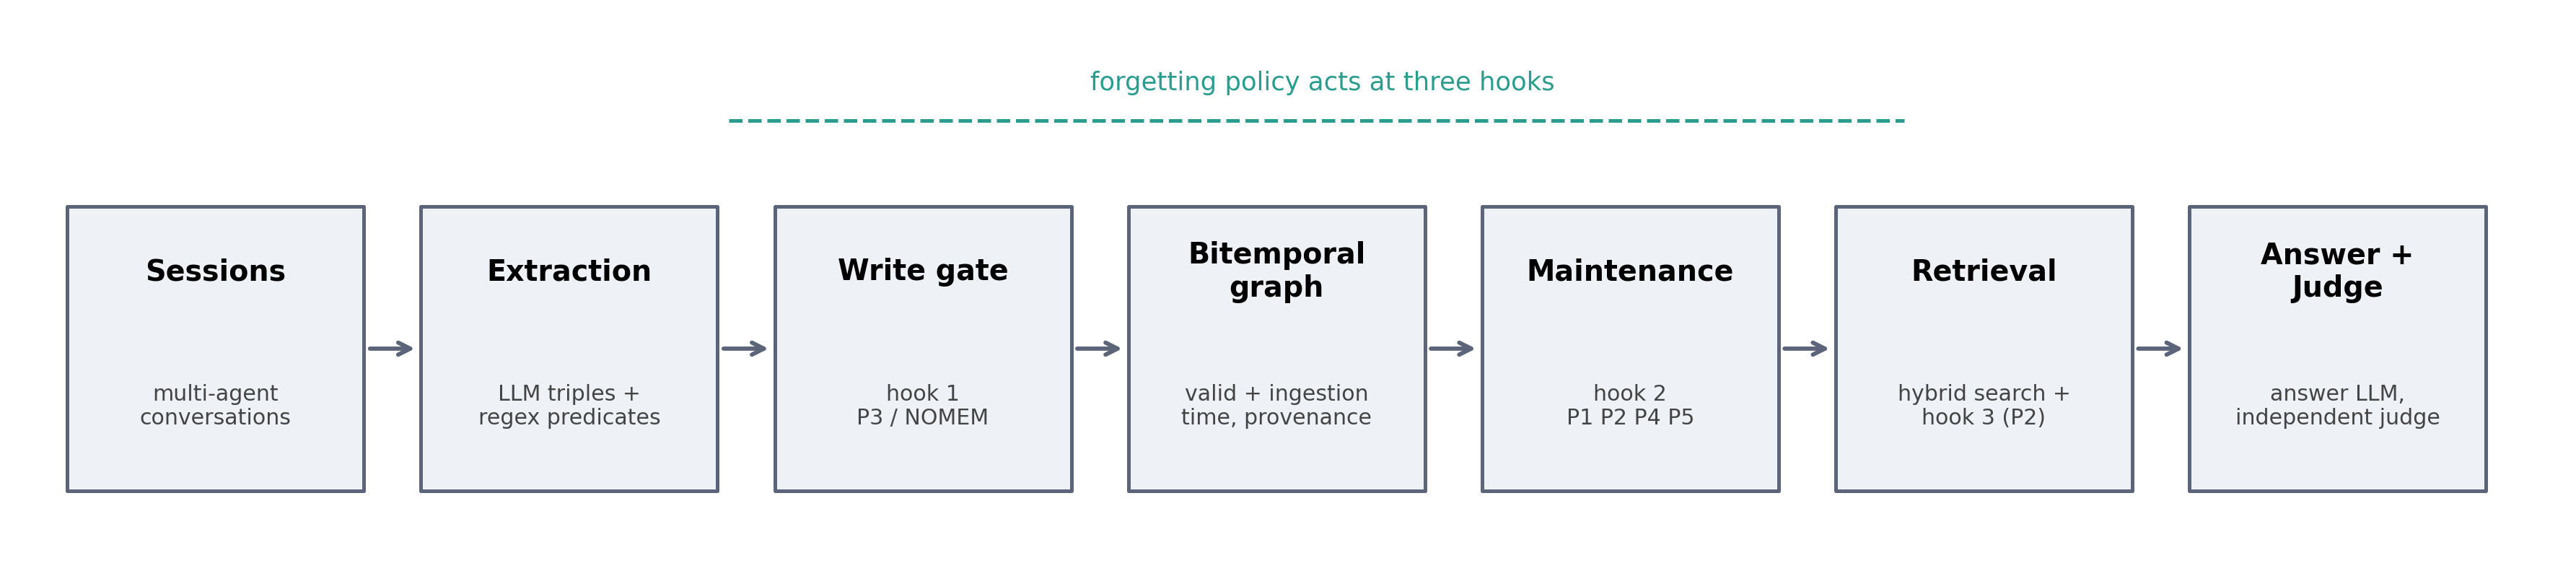
\includegraphics[width=0.85\textwidth]{figures/architecture.png}
\caption{The DRIFT pipeline. Session text is converted to facts, facts pass through the bitemporal substrate where contradictions on functional predicates close validity windows, a policy performs periodic maintenance, retrieval ranks candidate facts, a second policy hook filters or reranks what the answer model sees, and the answer is scored by an independent judge alongside a token-overlap metric.}
\label{fig:architecture}
\end{figure}

The stages, in order, are as follows. Session lines are converted into candidate facts by a language-model extraction step, backed by a deterministic regular-expression upgrade applied specifically to functional predicates, so that contradiction detection does not depend on the extractor happening to phrase two related facts identically. Each candidate fact is offered to the active policy's write hook, which may reject it outright before it ever enters the graph. Facts that are accepted enter the bitemporal knowledge graph, where a contradiction on a functional predicate closes the superseded fact's validity window in the non-destructive manner described in Section~\ref{sec:substrate}. After each session, the active policy's periodic-maintenance hook runs, which is where time-based pruning, grace-period pruning, language-model consolidation, or topology-based consolidation take place, depending on which policy is active. When a question is asked, retrieval ranks candidate facts by a fixed hybrid score combining cosine similarity, lexical overlap, and recency, weighted 0.6, 0.3, and 0.1 respectively, and returns the top $k = 25$ candidates. The active policy's retrieval hook then has the opportunity to filter or rerank this candidate set before it is handed to the answer model. The answer model produces a response, which is then scored twice: once by a large language model judge drawn from a different model family than the answer model, and once by a token-level F1 overlap metric that does not depend on a judge at all.

A policy is defined by exactly three hooks, shown in the interface below. Adding a new policy to the framework is a matter of subclassing this interface and registering the subclass; no other component of the pipeline, including the runner, the substrate, the model providers, or the analysis code, needs to be modified or even needs to be aware that a new policy exists.

\begin{verbatim}
class Policy:
    def on_write(self, fact, graph) -> bool:
        ...  # returning False rejects the write

    def after_session(self, graph, provider, now):
        ...  # periodic maintenance, run once per session

    def on_retrieve(self, facts, now) -> list:
        ...  # filter or rerank what the answer model sees
\end{verbatim}

\section{Policies Under Test}
\label{sec:policies}

Seven policies are compared, spanning a floor baseline, a ceiling baseline, and five distinct forgetting strategies. Table~\ref{tab:policies} summarizes each policy's mechanism and the hook or hooks it uses.

\begin{table}[H]
\centering
\caption{The seven policies compared in this thesis.}
\label{tab:policies}
\small
\begin{tabular}{lp{2.6cm}p{5.4cm}p{2.6cm}}
\toprule
ID & Name & Mechanism & Hooks used \\
\midrule
NOMEM & No memory & Retrieval returns nothing; a floor baseline & \texttt{on\_retrieve} \\
P0 & No forgetting & Append-only; nothing gated, pruned, or filtered; a ceiling baseline & none \\
P1 & TTL decay & Prune facts older than a fixed number of days by valid time & \texttt{after\_session} \\
P2 & Contradiction invalidation & Exclude superseded facts at retrieval time; prune after a seven-day grace period & \texttt{on\_retrieve}, \texttt{after\_session} \\
P3 & Novelty gate & Reject writes whose neighborhood cosine similarity exceeds a threshold of 0.9 & \texttt{on\_write} \\
P4 & LLM consolidation & Every third session, a language model decides which facts to keep or drop, plus a deterministic near-duplicate merge & \texttt{after\_session} \\
P5 & Topology consolidation & Resolve competing facts by structural corroboration count, deliberately denied access to valid time & \texttt{after\_session} \\
\bottomrule
\end{tabular}
\end{table}

\paragraph{NOMEM as a baseline.} The prompt given to the answer model instructs it to respond ``I don't know'' whenever memory does not contain the answer to a question. Under NOMEM, memory always fails to contain the answer, by construction, and the model's responses are almost entirely that refusal string, including in cases where the underlying language model plainly has the answer available from its own training. NOMEM therefore measures memory-gated answering behavior, not the model's parametric knowledge, and the gap between P0 and NOMEM should be read as the value memory adds under an explicit instruction to ground answers in memory rather than in general knowledge. A consequence worth stating plainly: NOMEM's staleness of exactly 0.000, reported in Chapter~\ref{chap:results}, is trivially achieved by refusing to answer at all, and staleness figures are only meaningfully comparable among policies that actually attempt an answer.

\paragraph{P5 as an ablation.} Policy P5 is not included because it is expected to perform well. It is included specifically to test whether the advantage of bitemporal reasoning comes from temporal information in particular, or merely from any form of graph-aware consolidation. P5 builds an entity co-occurrence graph from the same underlying facts P2 has access to, finds communities of related entities using label propagation, and within each community resolves competing facts sharing the same subject and predicate by retaining whichever candidate object is corroborated by the largest number of other facts elsewhere in memory. High-degree entities, meaning entities that participate in many facts, are protected from being pruned below a floor threshold. P5 has access to every structural signal P2 has access to, with the single exception of valid time.

\section{Metrics}
\label{sec:metrics}

Five quantities are reported for every experimental cell.

\paragraph{Accuracy.} A language model judge, drawn from a model family different from the answer model, returns a binary verdict of correct or incorrect against the gold answer for each question. Judges are drawn from a pool of three providers with automatic fallback between them; Section~\ref{sec:judge-audit} audits the consequences of this rotation for the reliability of the accuracy metric itself.

\paragraph{Staleness.} The fraction of answers that contain the superseded value for a question, computed as a case-insensitive substring test between the model's answer and the question's annotated \texttt{stale\_answer} field:

\begin{verbatim}
def staleness_hit(answer, stale_answer):
    if not stale_answer:
        return False
    return stale_answer.lower() in answer.lower()
\end{verbatim}

Staleness can only fire on questions that carry a \texttt{stale\_answer} annotation, which means a benchmark's annotation coverage places a hard upper bound on what this metric is capable of reporting for that benchmark. This is not a minor caveat; it is the subject of Section~\ref{sec:benchmark-selection}, and it is the source of a false result the author initially mistook for a finding before diagnosing its cause.

\paragraph{Token-F1.} Unigram overlap between the model's answer and the gold answer, reported alongside accuracy because it does not depend on a judge at all. It penalizes verbose answers, which is why the two answer models used in this thesis diverge sharply on this metric while agreeing closely on judge-scored accuracy; Section~\ref{sec:per-model} discusses this divergence and its implication for metric selection.

\paragraph{Cost.} The mean number of tokens consumed per question at answer time, together with the count of facts the policy retains as active in memory at the end of the run.

\paragraph{Retrieved-invalidated.} The mean number of facts appearing in a retrieval that have had their validity window closed by a contradiction. This is the mechanism variable underlying the staleness metric: it is exactly 0.00 for policy P2 by construction, because P2's retrieval hook filters such facts out before the answer model ever sees them, and it ranges from roughly 4.2 to 5.4 for the policies that do not filter on this basis.

\section{Statistics}
\label{sec:statistics}

Four statistical procedures are used throughout Chapter~\ref{chap:results}, chosen specifically because the design compares policies that are evaluated on the identical set of questions rather than on independent samples.

\begin{itemize}
\item \textbf{Bootstrap 95 percent confidence intervals}, computed by the percentile method with 5,000 resamples, reported for every accuracy and staleness figure.
\item \textbf{Paired McNemar exact test}, using the exact two-sided binomial distribution over discordant pairs, for comparing two policies on the same set of questions. Because every policy answers the identical question set, an unpaired test would overstate the significance of an observed difference by treating correlated outcomes as independent.
\item \textbf{Paired bootstrap on the per-question difference}, used to estimate effect sizes. This procedure is a stronger form of evidence than comparing two overlapping confidence intervals computed independently for each policy, and it is what allows a failure to reject a null hypothesis to be reported as a bounded equivalence claim rather than as an inconclusive result, a distinction developed at length in Section~\ref{sec:rq2}.
\item \textbf{Spearman's rank correlation}, computed on the policy rankings produced by each benchmark, used to quantify how well a ranking established on one benchmark generalizes to a second benchmark of different provenance.
\end{itemize}
   % Method
\chapter{Experimental Setup}
\label{chap:experimental-setup}

This chapter describes how the benchmarks used in this thesis were selected, including a negative result that shaped the entire experimental design, the two benchmarks ultimately used and how each was adapted to DRIFT's evaluation schema, the models and infrastructure involved, and the measures taken to ensure the results are reproducible.

\section{Benchmark Selection, and a Negative Result About the Standard Benchmarks}
\label{sec:benchmark-selection}

The staleness metric defined in Section~\ref{sec:metrics} requires each question in a benchmark to be annotated with the value a stale memory would return for that question, referred to as the \texttt{stale\_answer} annotation. Before committing to any benchmark, every reasonable candidate was audited for this annotation, with the results shown in Table~\ref{tab:benchmark-audit}.

\begin{table}[H]
\centering
\caption{Audit of \texttt{stale\_answer} annotation coverage across candidate benchmarks.}
\label{tab:benchmark-audit}
\small
\setlength{\tabcolsep}{4pt}
\begin{tabular}{p{3.2cm}rrrrrr}
\toprule
Benchmark & Conv. & Sessions & Lines & Questions & With annot. & Coverage \\
\midrule
LoCoMo & 10 & 272 & 5{,}882 & 300 & 0 & 0\% \\
LongMemEval & n/a & n/a & n/a & 150 & 0 & 0\% \\
LongMemEval, LLM-annotated & 78 & 156 & 1{,}830 & 78 & 1 & 1\% \\
FactConsolidation & 1 & 38 & 380 & 100 & 65 & 65\% \\
MQuAKE-T & 1 & 38 & 382 & 96 & 96 & 100\% \\
Synthetic smoke (offline) & 2 & 10 & 28 & 14 & 4 & 29\% \\
\bottomrule
\end{tabular}
\end{table}

This table exists because of a mistake made and corrected during the course of this research, and it is reported in full because the same mistake is available to anyone else working in this area. On the first experimental campaign, staleness read exactly 0.000 across all forty-two single-agent experimental cells run at that time. For a brief period this reading was interpreted as a substantive finding, namely that none of the policies under test were producing stale answers. It was not a finding. The staleness metric could not fire in principle on that data, because the annotation it depends on, \texttt{stale\_answer}, does not exist anywhere in LoCoMo or in the standard LongMemEval question set. A metric that structurally cannot fire will always read zero, and a reading of zero produced by the metric's own inapplicability is indistinguishable, from the summary statistics alone, from a reading of zero produced by policies that are genuinely working well.

This is reported here as a negative result in its own right, distinct from the positive results reported in Chapter~\ref{chap:results}, because the same trap is available to any researcher measuring memory revision on LoCoMo or on LongMemEval, and because the diagnostic that exposes it is simple: any staleness result reported for a benchmark should be accompanied by that benchmark's annotation coverage. The cross-dataset comparison tool built for this thesis prints this coverage figure automatically for exactly this reason, so that the same mistake cannot recur silently in a later run.

An attempt was also made to recover the missing annotation for LongMemEval's knowledge-update question subset using a language model annotator, prompted to identify the superseded value from the evidence turns of each conversation. This attempt produced one usable annotation out of seventy-eight questions, despite the superseded values appearing in plain, unambiguous text in the evidence turns themselves, for example a phone extension of ``27:12,'' a dollar figure of ``\$350,000,'' or a frequency of ``twice a week.'' The annotator's failure to recover values that are present verbatim in its own input suggests that the difficulty lies in the annotation task itself rather than in the specific prompt used, and it is the reason this thesis relies on deterministic recovery of the superseded value from a benchmark's own structure, described for each benchmark in Section~\ref{sec:two-benchmarks}, rather than on an automated annotator.

\section{The Two Benchmarks Used}
\label{sec:two-benchmarks}

Two benchmarks satisfy the annotation requirement well enough to support this thesis's experiments: FactConsolidation, drawn from MemoryAgentBench, and MQuAKE-T, drawn from MQuAKE.

\paragraph{FactConsolidation.} FactConsolidation is a split of MemoryAgentBench consisting of a numbered list of facts in which later facts overwrite earlier facts sharing the same subject and predicate, with the gold answer to each question always being the most recent value \citep{hu2026memoryagentbench}. The superseded value for each question is recoverable without a human or automated annotator, by tracking the previous object of whichever subject-predicate pair ultimately resolves to the gold answer. Because facts in this benchmark are presented as atomic triples rather than embedded in free-form conversation, contradiction detection is not bottlenecked by extraction quality, which makes FactConsolidation a clean setting in which to isolate the behavior of the forgetting policies themselves. Gold answers in this benchmark are deliberately counterfactual, for example the claim that rugby union was created in India, which means a language model's own parametric knowledge is actively unhelpful and cannot be used to guess the correct answer without consulting memory.

\paragraph{MQuAKE-T.} MQuAKE-T is built by comparing Wikidata snapshots taken in April 2021 and April 2023, and retaining relations whose value changed in a way that reflects a genuine real-world update rather than a synthetic edit \citep{zhong2023mquake}. Each instance in the resulting dataset ships both the pre-edit answer and the post-edit answer, so the \texttt{stale\_answer} annotation is deterministic and requires no separate annotation step. MQuAKE-T was selected specifically as the generalization test for this thesis because its updates are real rather than injected, which removes the most artificial property of FactConsolidation, namely that its supersessions are constructed by the benchmark's authors rather than observed in the world, while holding the underlying task form, a fact list followed by questions about the current value, fixed between the two benchmarks.

The conversion of MQuAKE-T into DRIFT's dataset schema was sized to match FactConsolidation cell for cell, as shown in Table~\ref{tab:benchmark-sizing}, so that a comparison between the two benchmarks reflects a difference in the nature of the data rather than a difference in scale.

\begin{table}[H]
\centering
\caption{Sizing comparison between the two benchmarks used.}
\label{tab:benchmark-sizing}
\begin{tabular}{lrr}
\toprule
Property & FactConsolidation & MQuAKE-T \\
\midrule
Sessions & 38 & 38 \\
Fact lines & 380 & 382 \\
Questions & 100 & 96 \\
\texttt{stale\_answer} coverage & 65\% & 100\% \\
Policies $\times$ answer models & $7 \times 2 = 14$ cells & $7 \times 2 = 14$ cells \\
Question-answers pooled & 200 & 192 \\
\bottomrule
\end{tabular}
\end{table}

Two decisions made during the conversion of MQuAKE-T are load-bearing for the validity of the results reported in Chapter~\ref{chap:results}, and both are stated explicitly here so they can be scrutinized rather than discovered later.

\paragraph{Randomized supersession placement.} For each edited fact pair, the old value is placed in a uniformly random session $i$ and the new value in a uniformly random later session $j > i$, rather than placing all old values into an early block of sessions and all new values into a late block. A clean chronological boundary between old and new values would let any policy that simply favors more recent sessions in general appear to win, without that policy ever needing to use bitemporal structure specifically. This is exactly the confound the ablation comparing bitemporal invalidation against structure-blind, time-blind consolidation, described in Section~\ref{sec:rq3}, is designed to rule out, and randomizing the placement of old and new values is what makes that ablation a fair test rather than a foregone conclusion.

\paragraph{Flat statement phrasing.} Edited facts are restated in compact subject-predicate-object form, for example ``The head of government of New York City is Eric Adams,'' rather than in MQuAKE's original cloze-style phrasing, for example ``The name of the current head of the New York City government is.'' Contradiction detection depends on the extraction step producing the same subject and predicate for a fact and for the fact that later corrects it, and a longer, more grammatically varied phrasing introduces extraction variance on precisely the one join the entire experiment depends on. The original cloze phrasing is retained in the conversion script behind a configuration flag, so that the trade-off between phrasing style and extraction reliability can itself be measured in future work rather than being a silent, unexamined choice.

\section{Models and Infrastructure}
\label{sec:models-infra}

Table~\ref{tab:models} lists the models used in each role in the pipeline.

\begin{table}[H]
\centering
\caption{Models and infrastructure used in every experimental cell.}
\label{tab:models}
\begin{tabular}{ll}
\toprule
Role & Models \\
\midrule
Answer & GLM-5.2, MiniMax-M3 (via OpenRouter) \\
Extraction & GLM-5.2, MiniMax-M3, gpt-oss-120b, Llama-3.3-70B, \\
 & Llama-3.1-8B, Mistral Small (rotated per conversation) \\
Judge & gpt-oss:20b (local), gpt-oss-20b (hosted), Command-R7B \\
 & (rotated per conversation) \\
Embedding & \texttt{nomic-embed-text}, served locally via Ollama, 768 dimensions \\
Retrieval depth & $k = 25$ \\
\bottomrule
\end{tabular}
\end{table}

Extraction and judging both rotate across a pool of providers, chosen specifically to spread the volume of API calls generated by a full campaign across independent rate limits rather than exhausting a single provider's quota. Section~\ref{sec:judge-audit} shows that this rotation, while necessary for completing a campaign of this size in practice, is also a confound affecting the reliability of the accuracy metric, and recommends pinning a single judge for any run whose numbers will be reported.

\section{Reproducibility}
\label{sec:reproducibility}

Several measures were taken during development to ensure that every number reported in Chapter~\ref{chap:results} can be regenerated exactly, and to reduce the practical cost of doing so.

\begin{itemize}
\item Every call made to a model provider is cached to disk, keyed by the SHA-256 hash of the tuple (provider, model, prompt, temperature, max tokens). An interrupted campaign resumes at zero additional cost, because every call already completed is served from the cache rather than repeated, and a rerun of a completed campaign is bit-for-bit reproducible, because the same inputs always retrieve the same cached outputs.
\item Results are written one file per experimental cell, and cells that have already completed are automatically skipped on a subsequent invocation, which makes a large campaign safely resumable after an interruption of any kind.
\item Failures are caught at the level of an individual cell rather than at the level of an entire campaign, so that one provider running out of quota, or one transient network failure, costs a single cell rather than terminating the whole run.
\item A deterministic, offline mock provider and a deterministic, offline hashing-based embedder allow the entire pipeline to be exercised without any network access and without any API key. The complete test suite, which exercises this offline path, runs 99 tests in a fraction of a second, which means the mechanics of the pipeline can be verified independently of, and prior to, any claim about the reported results themselves.
\item The core package that implements the framework declares zero external dependencies, which removes an entire category of reproducibility failure caused by dependency version drift between the environment the results were produced in and the environment a reader later attempts to reproduce them in.
\end{itemize}

Appendix~\ref{app:reproduction} gives the exact command sequence needed to regenerate every table and figure in Chapter~\ref{chap:results} from a clean checkout of the codebase.
   % Experimental Setup
\chapter{Results}
\label{chap:results}

This chapter reports the experimental results of this thesis, organized around the four research questions stated in Section~\ref{sec:research-questions}, together with two methodological results, a configuration ablation and a judge-reliability audit, that emerged while reconciling experimental runs against one another. All figures quoted in this chapter are computed from the result files produced by the experimental runs and can be regenerated exactly using the commands given in Appendix~\ref{app:reproduction}. The complete per-cell results underlying every table in this chapter, and the full pairwise significance matrix across all twenty-one policy pairs, are given in Appendix~\ref{app:results}.

\section{Headline Results}
\label{sec:headline}

Tables~\ref{tab:headline} and~\ref{tab:headline-mq} report accuracy, staleness, token cost, and active fact count for all seven policies, pooled across both answer models, on FactConsolidation and MQuAKE-T respectively. Confidence intervals are percentile bootstrap at the 95 percent level with 5,000 resamples. The sample size is 200 question-answer pairs on FactConsolidation and 192 on MQuAKE-T.

Table~\ref{tab:headline} is reported as two panels, one per benchmark, since every column for both benchmarks side by side does not fit within a portrait page margin at a legible size.

\begin{table}[H]
\centering
\caption{Headline results, FactConsolidation. Bold marks the best value in a column among the policies that answer (NOMEM excluded).}
\label{tab:headline}
\small
\begin{tabular}{lcccc}
\toprule
Policy & Accuracy & Staleness & Tok/q & Facts \\
\midrule
NOMEM & 0.000 [.000,.000] & 0.000 & 250 & n/a \\
\textbf{P0} & \textbf{0.840} [.785,.890] & 0.030 [.010,.055] & 812 & 380 \\
P1 (TTL 20d) & 0.630 [.565,.695] & 0.020 [.005,.040] & 799 & 210 \\
\textbf{P2} & \textbf{0.840} [.785,.890] & 0.025 [.005,.050] & \textbf{715} & \textbf{324} \\
P3 & 0.665 [.600,.730] & \textbf{0.140} [.095,.190] & 806 & 334 \\
P4 & 0.800 [.745,.855] & 0.060 [.030,.095] & 814 & 374 \\
P5 & 0.795 [.735,.850] & 0.035 [.010,.060] & 812 & 365 \\
\bottomrule
\end{tabular}
\end{table}

\begin{table}[H]
\centering
\caption{Headline results, MQuAKE-T. Bold marks the best value in a column among the policies that answer (NOMEM excluded).}
\label{tab:headline-mq}
\small
\begin{tabular}{lcccc}
\toprule
Policy & Accuracy & Staleness & Tok/q & Facts \\
\midrule
NOMEM & 0.000 [.000,.000] & 0.000 & 233 & n/a \\
\textbf{P0} & \textbf{0.969} [.943,.990] & 0.052 [.021,.089] & 816 & 382 \\
P1 (TTL 20d) & 0.870 [.823,.917] & 0.026 [.005,.052] & 807 & 251 \\
\textbf{P2} & \textbf{0.969} [.943,.990] & 0.036 [.010,.068] & \textbf{716} & \textbf{357} \\
P3 & 0.792 [.729,.849] & \textbf{0.161} [.109,.214] & 805 & 351 \\
P4 & 0.953 [.922,.979] & 0.057 [.026,.094] & 804 & 372 \\
P5 & 0.802 [.745,.854] & \textbf{0.214} [.156,.276] & 816 & 365 \\
\bottomrule
\end{tabular}
\end{table}

Figure~\ref{fig:accuracy-staleness} plots this table directly. Figure~\ref{fig:tradeoff} places each policy in accuracy-staleness space, and Figure~\ref{fig:token-cost} plots the token-cost column.

\begin{figure}[H]
\centering
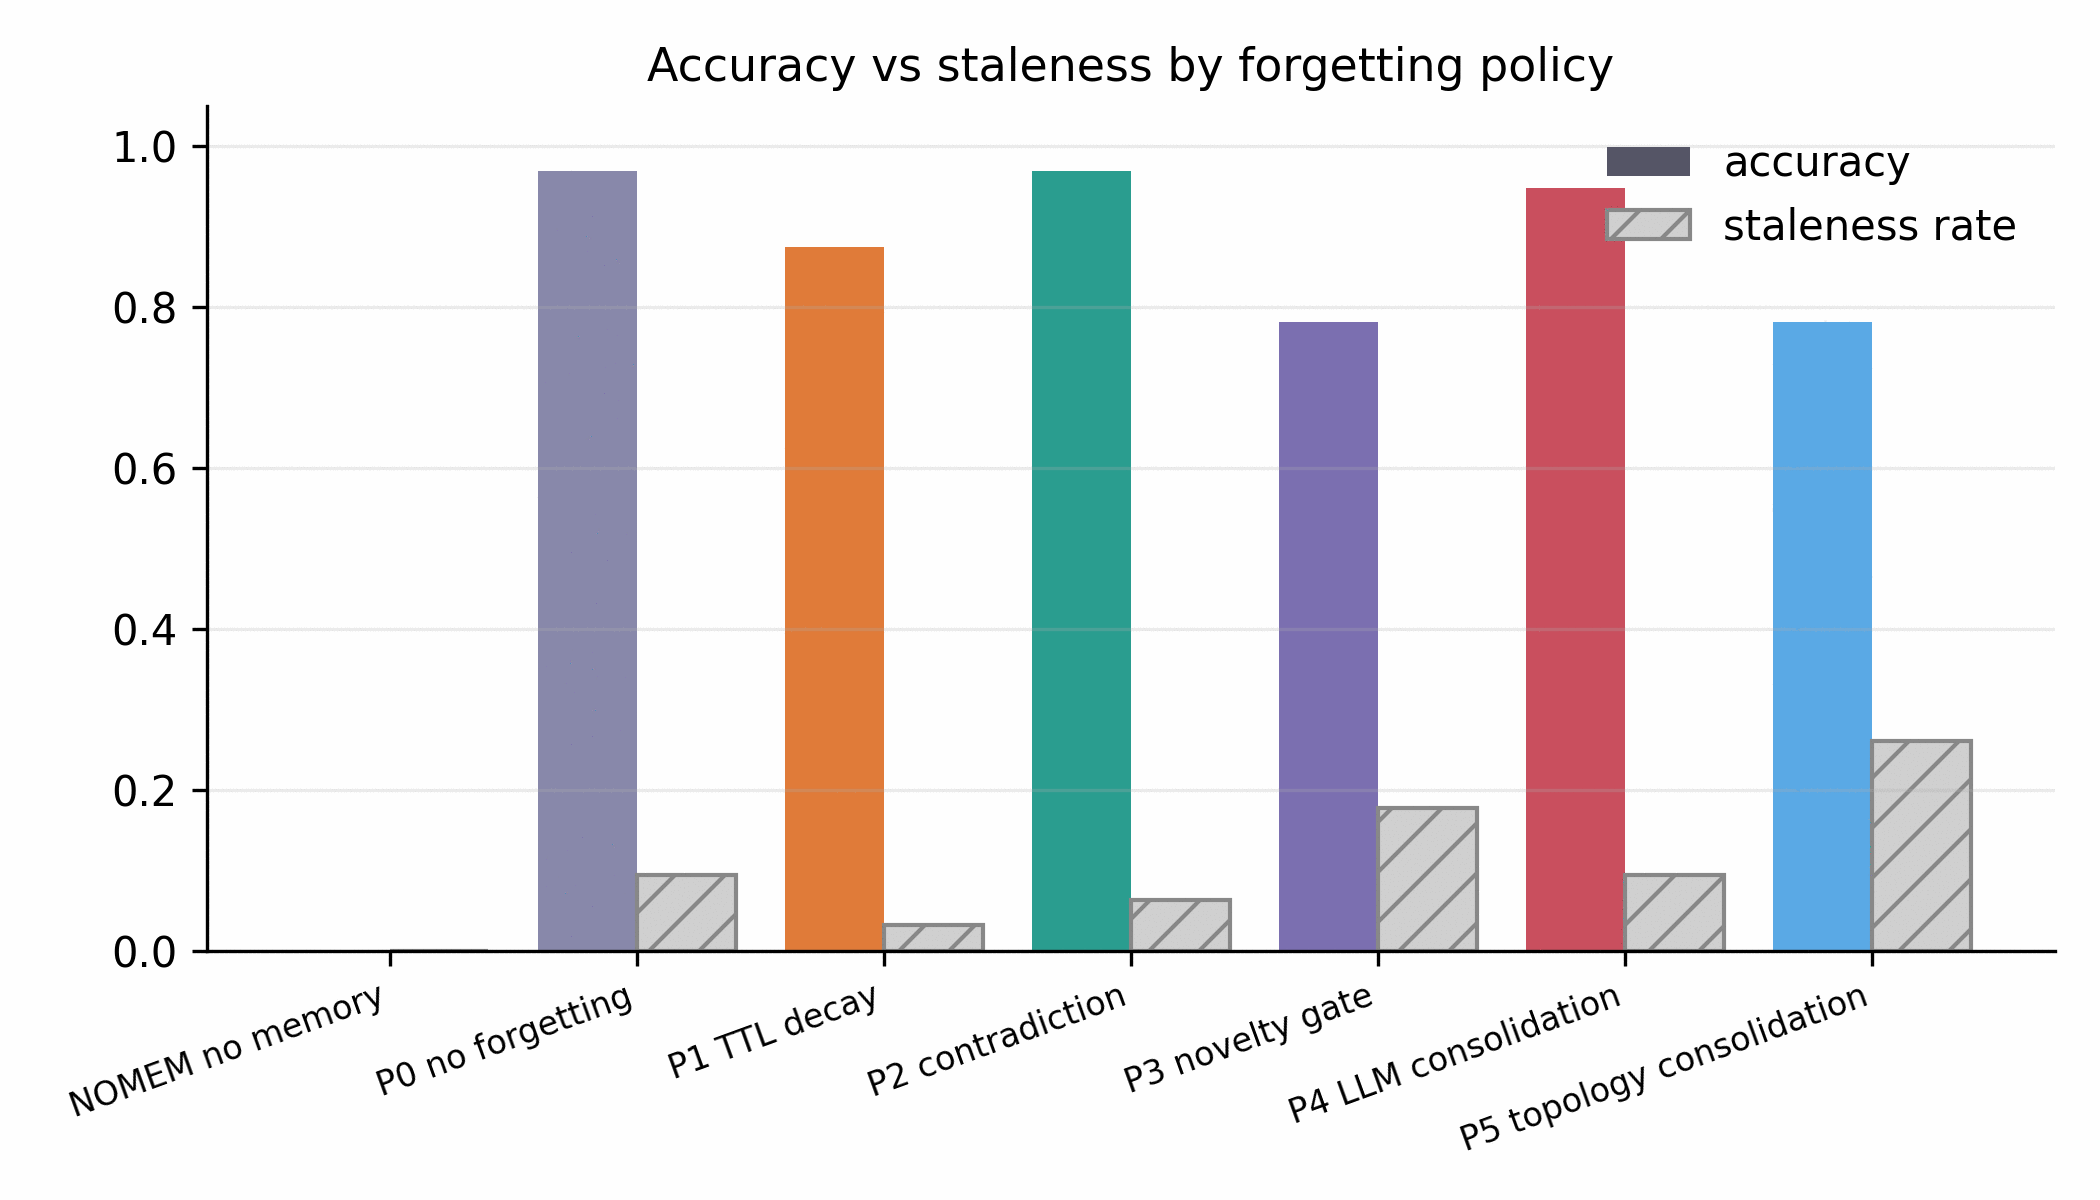
\includegraphics[width=0.85\textwidth]{figures/accuracy_staleness_mquake_t.png}
\caption{Accuracy and staleness by policy, MQuAKE-T.}
\label{fig:accuracy-staleness}
\end{figure}

\begin{figure}[H]
\centering
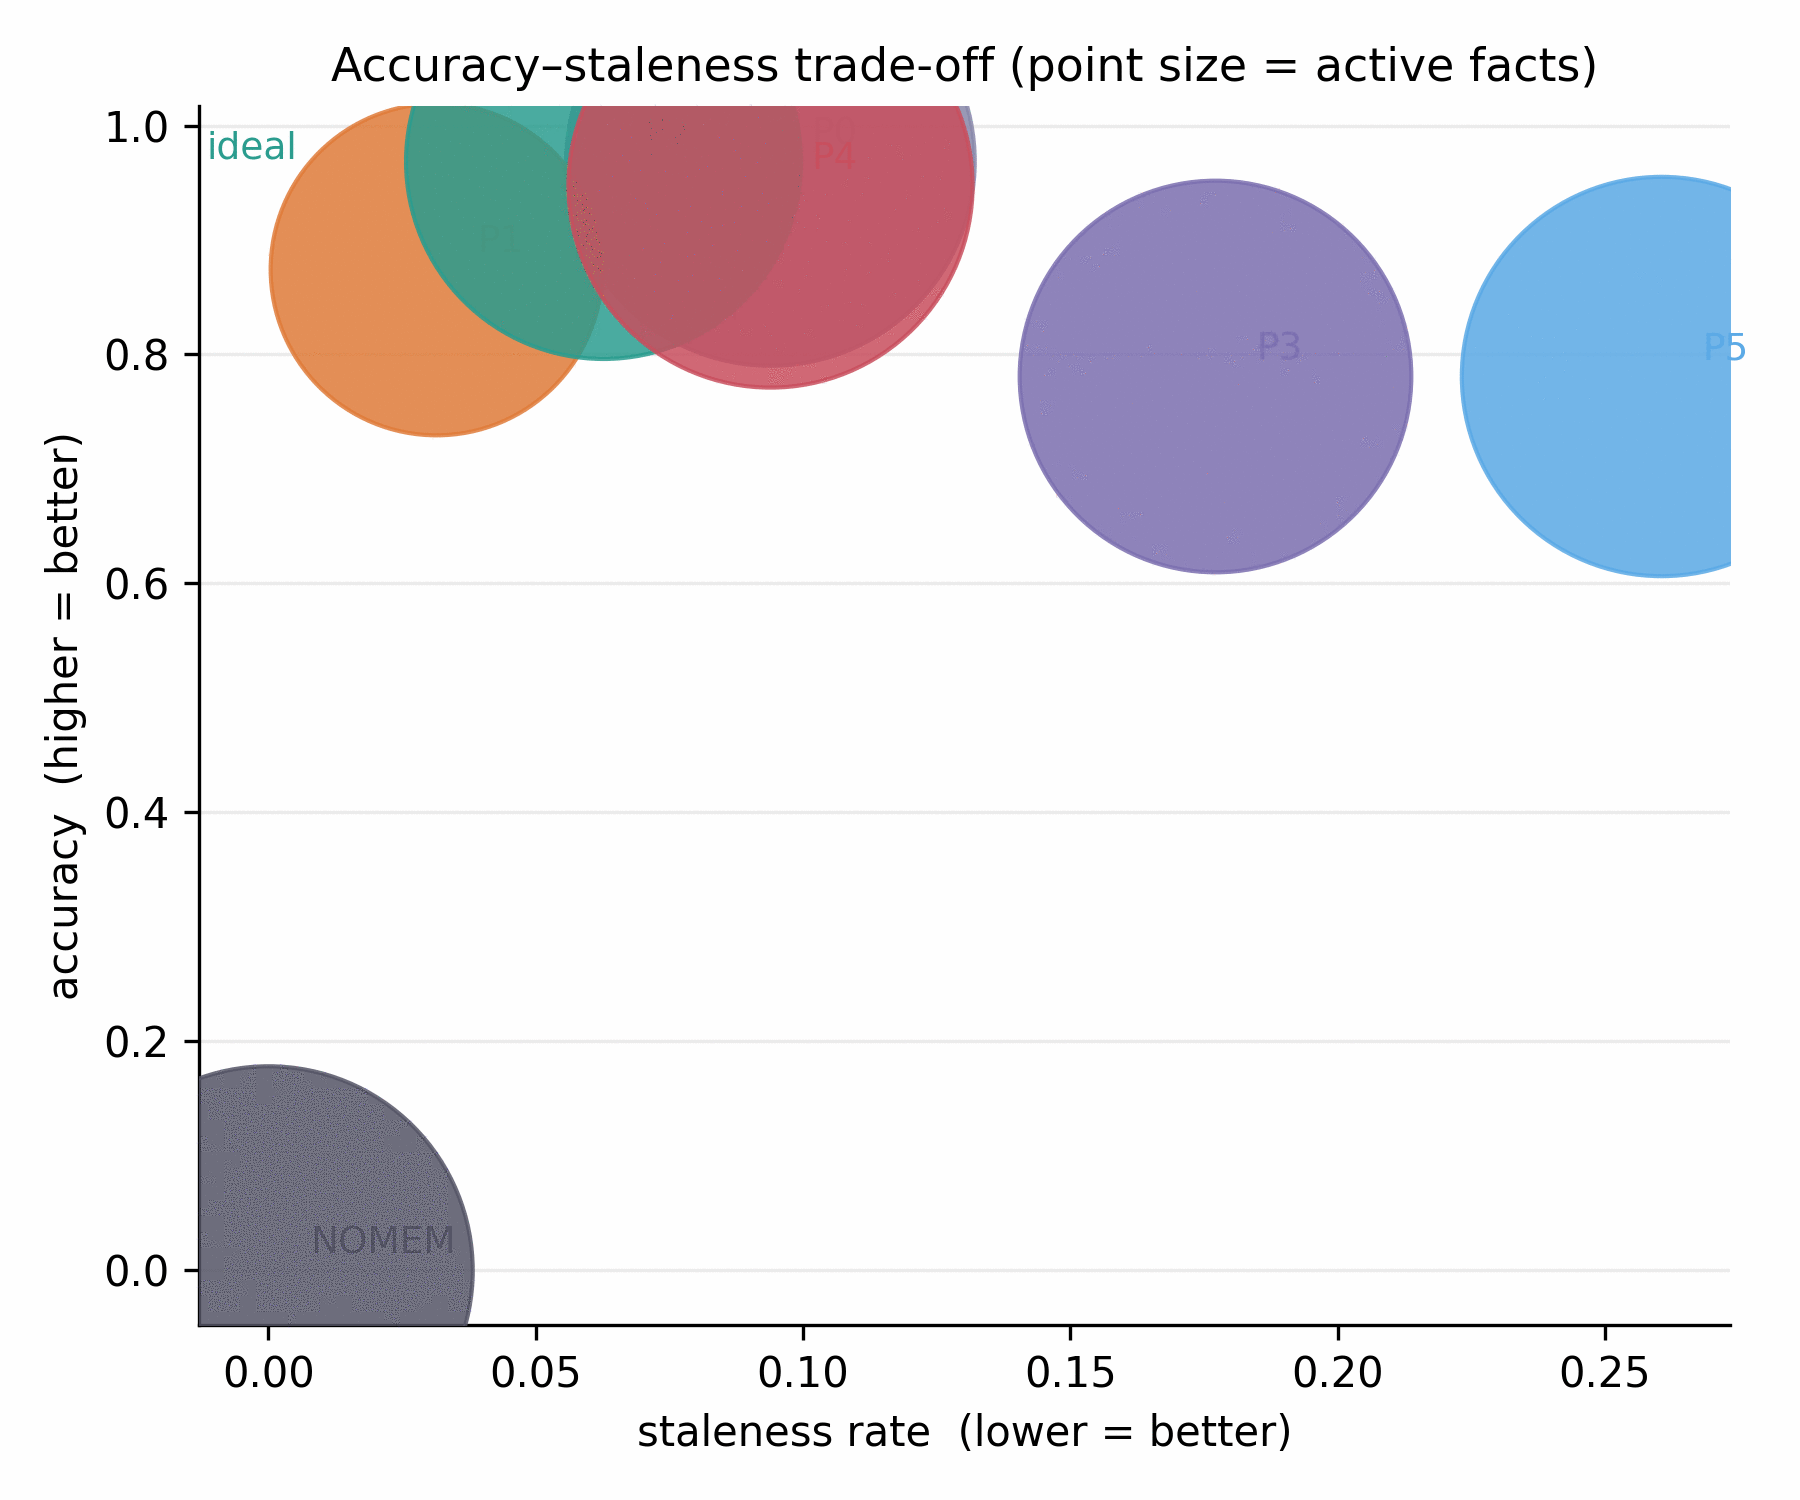
\includegraphics[width=0.75\textwidth]{figures/tradeoff_scatter_mquake_t.png}
\caption{Accuracy plotted against staleness for each policy, MQuAKE-T. The policy closest to the top left corner has the best combined profile.}
\label{fig:tradeoff}
\end{figure}

\begin{figure}[H]
\centering
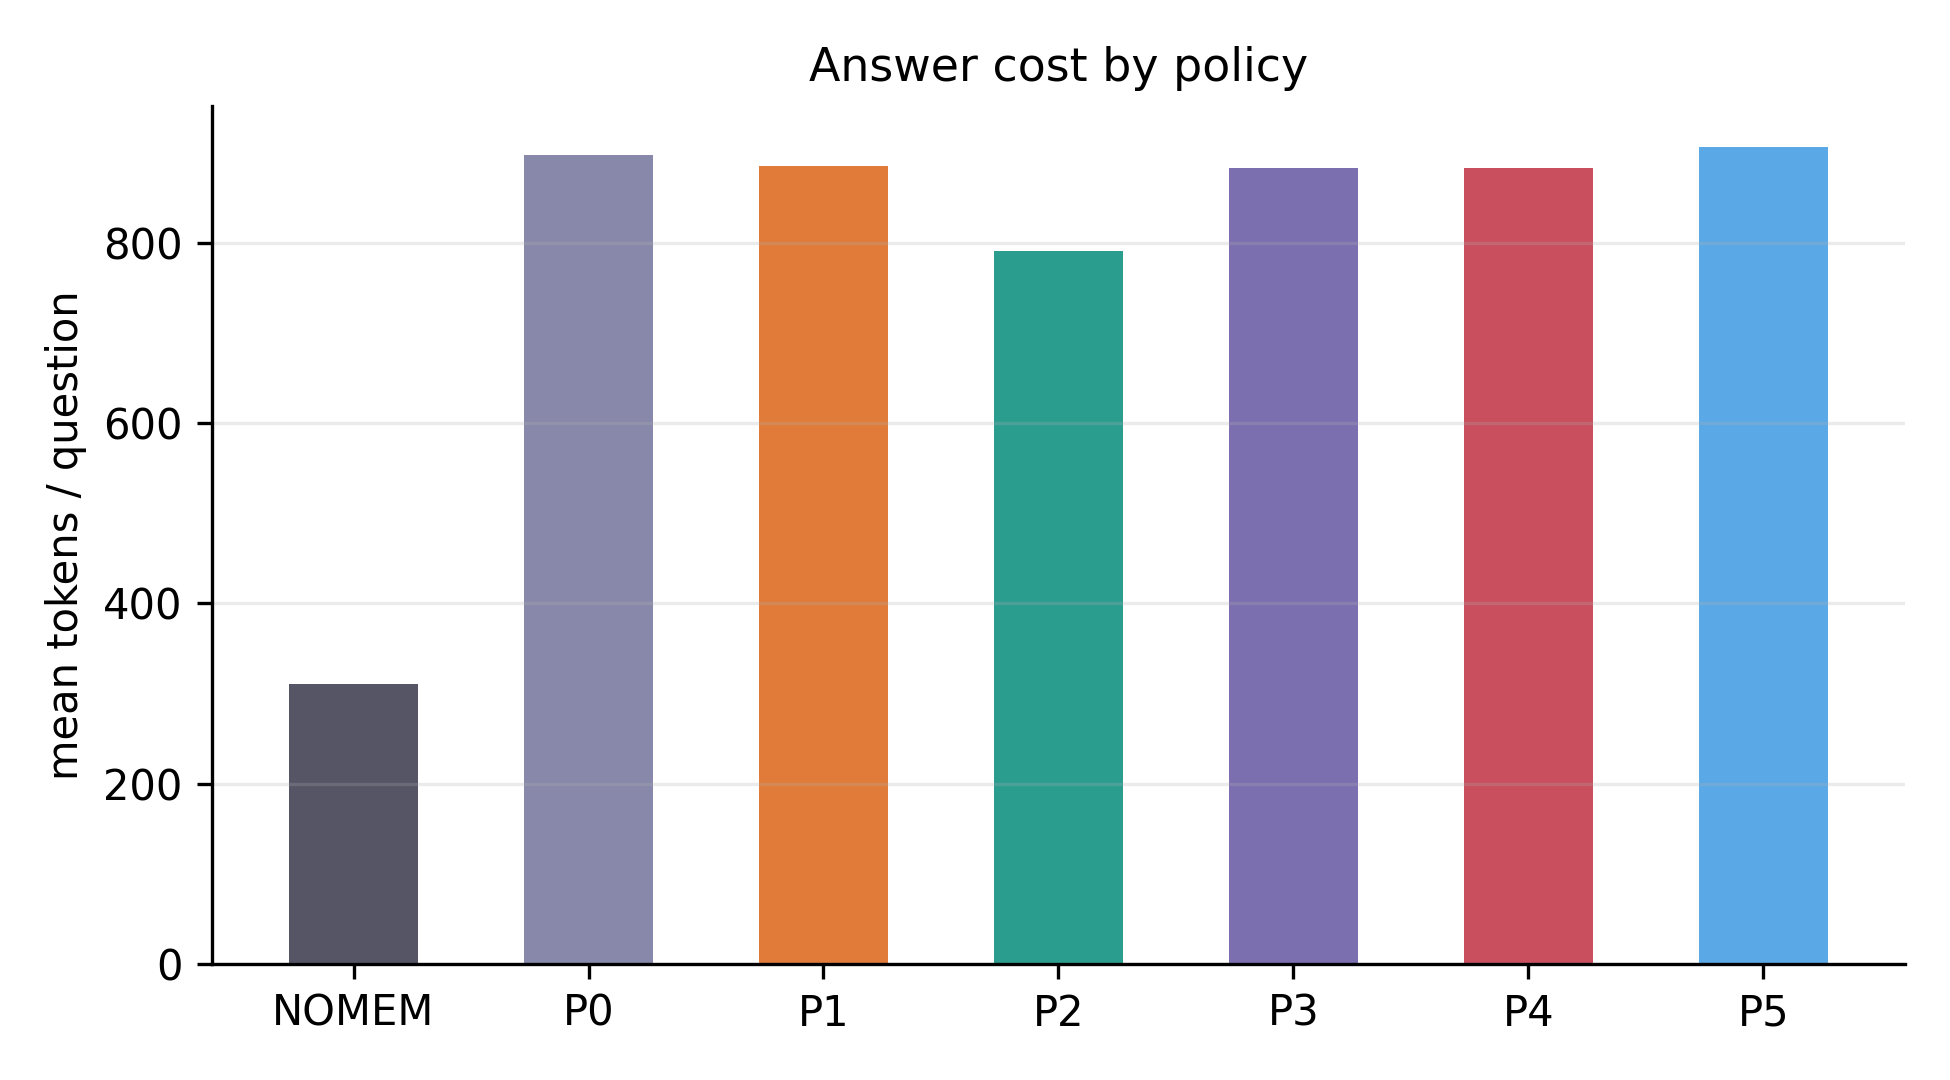
\includegraphics[width=0.75\textwidth]{figures/token_cost_mquake_t.png}
\caption{Mean tokens consumed per question, by policy, MQuAKE-T.}
\label{fig:token-cost}
\end{figure}

\begin{figure}[H]
\centering
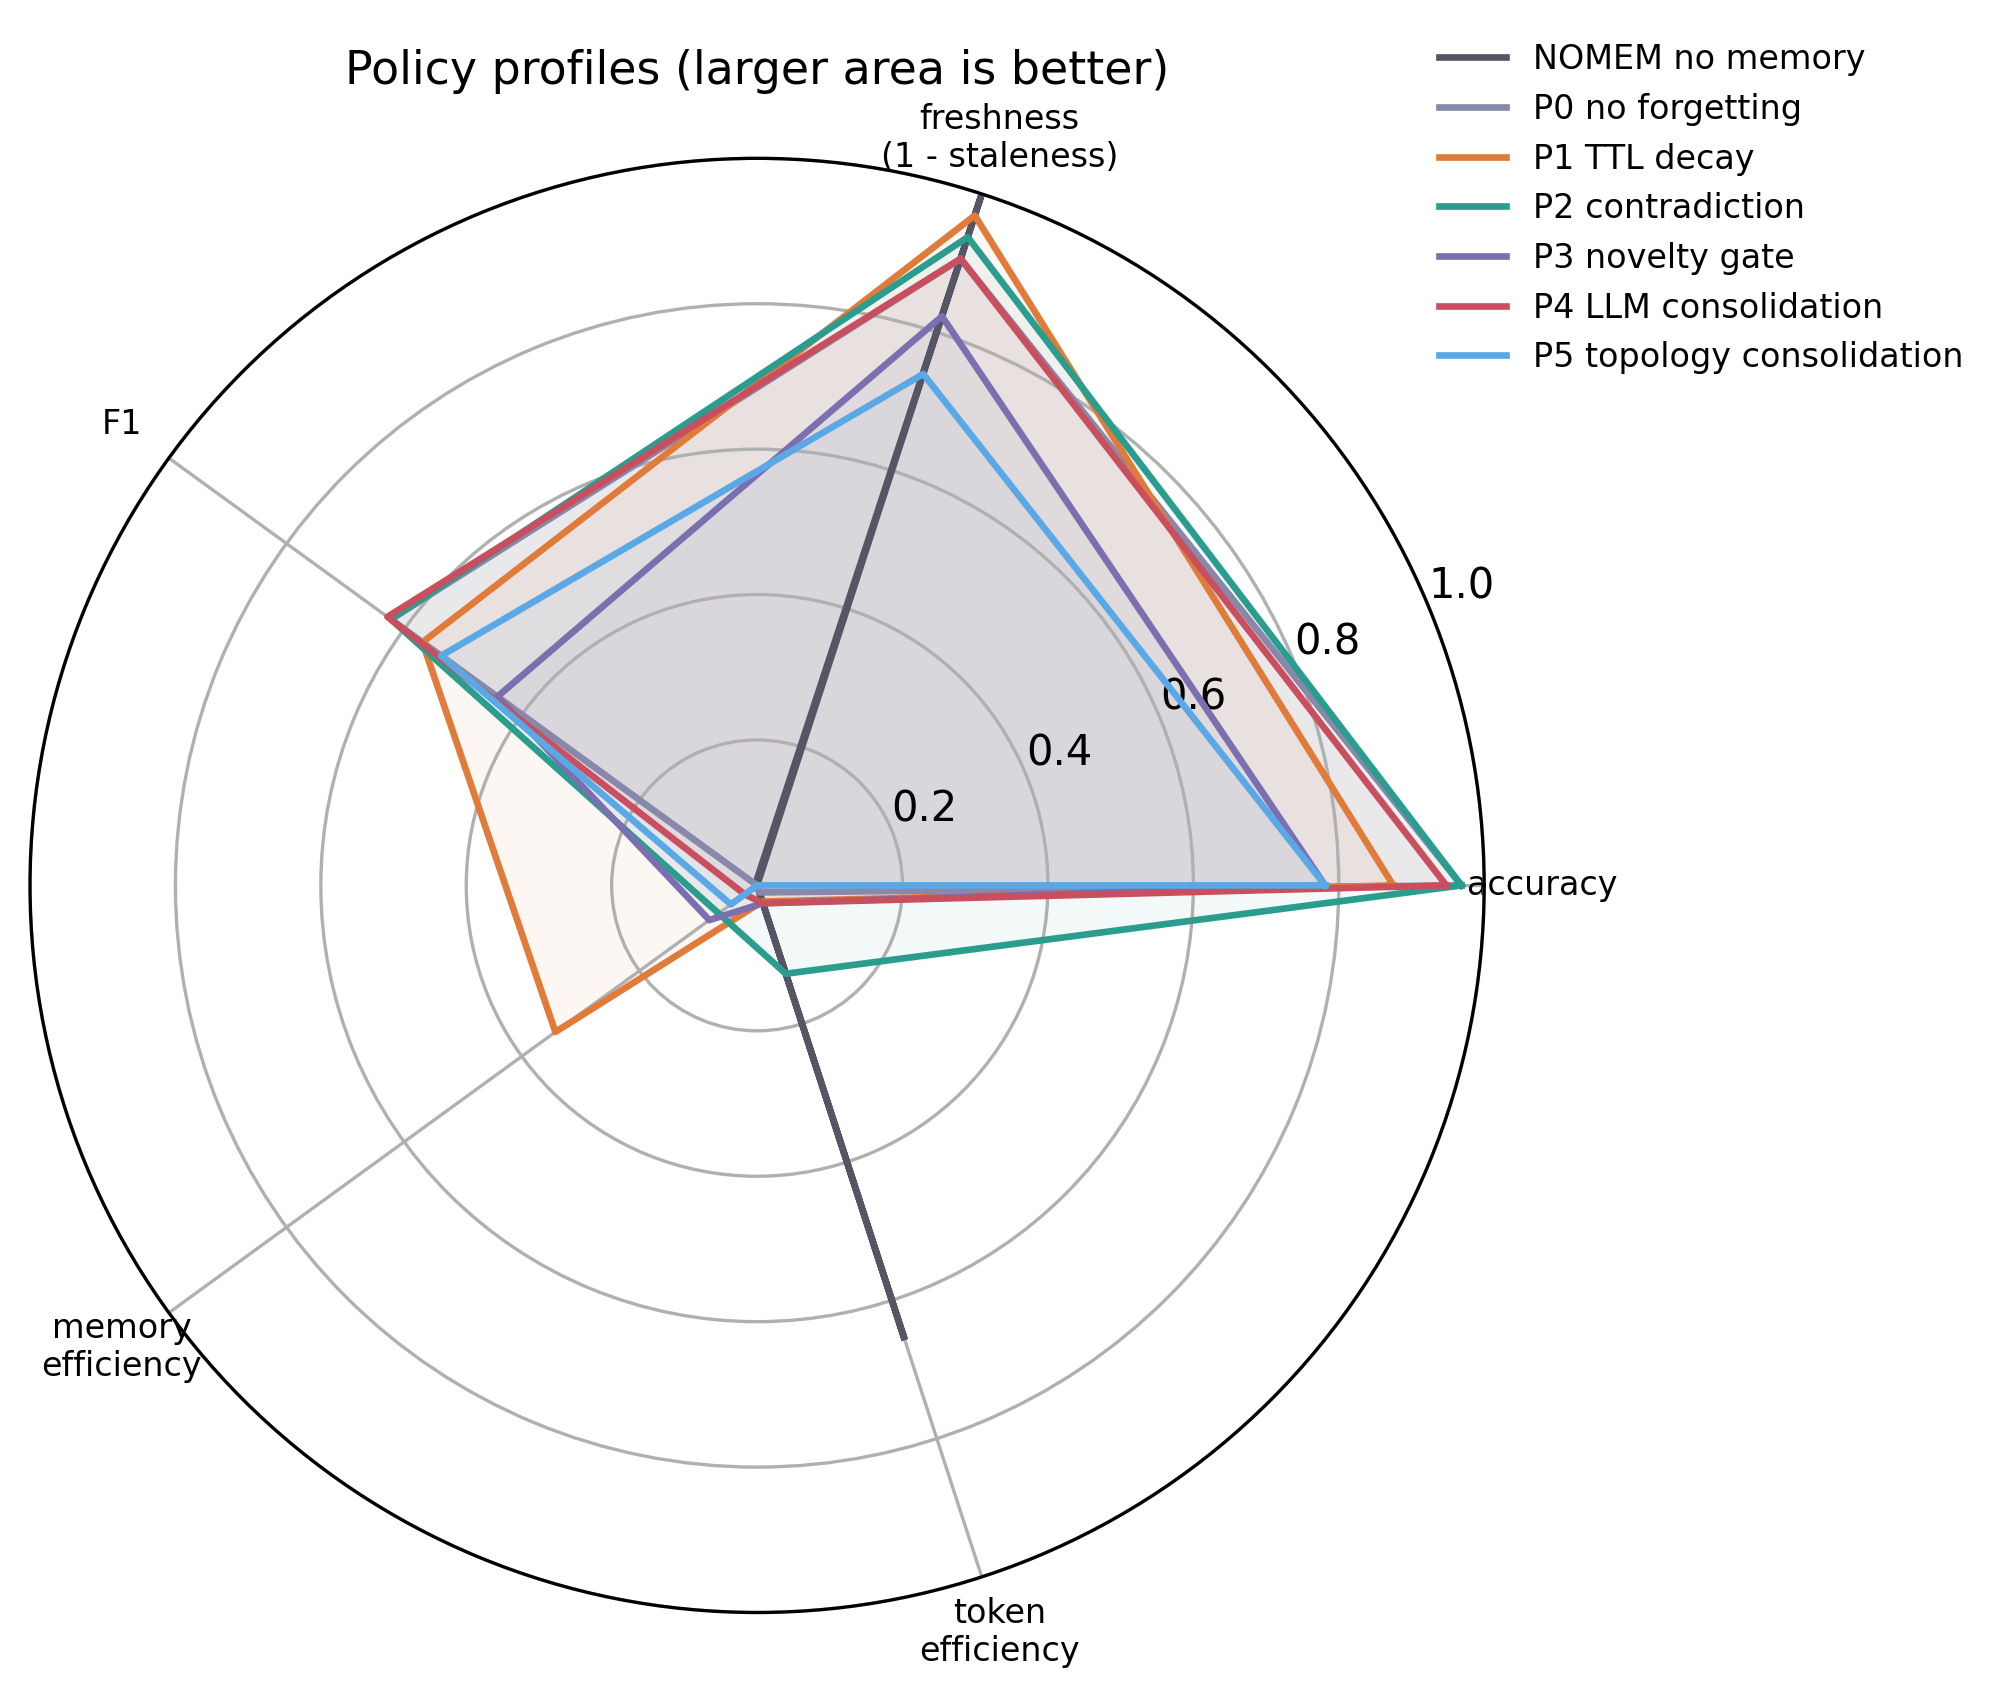
\includegraphics[width=0.7\textwidth]{figures/radar_policies_mquake_t.png}
\caption{All seven policies compared across every reported metric simultaneously, MQuAKE-T.}
\label{fig:radar}
\end{figure}

\section{Effect Sizes with Paired Bootstrap Intervals}
\label{sec:effect-sizes}

Comparing two independently computed confidence intervals for overlap is a weak form of evidence, because it does not use the fact that every policy is evaluated on the same set of questions. Table~\ref{tab:effect-sizes} instead bootstraps the paired per-question difference directly, which is the correct estimator whenever the compared conditions share their evaluation set, as is the case for every comparison in this thesis.

\begin{table}[H]
\centering
\caption{Effect sizes from paired bootstrap on the per-question difference. FC is FactConsolidation, MQ is MQuAKE-T.}
\label{tab:effect-sizes}
\small
\setlength{\tabcolsep}{4pt}
\begin{tabular}{llllll}
\toprule
Bench. & Comparison & Metric & Delta & 95\% CI & Excl. 0 \\
\midrule
FC & P2 minus P0 & accuracy & +0.000 & [-0.025, +0.025] & no \\
FC & P2 minus P0 & staleness & -0.005 & [-0.035, +0.025] & no \\
FC & P2 minus P3 & accuracy & +0.175 & [+0.120, +0.230] & yes \\
FC & P2 minus P3 & staleness & -0.115 & [-0.165, -0.070] & yes \\
FC & P2 minus P5 & accuracy & +0.045 & [+0.015, +0.080] & yes \\
FC & P2 minus P5 & staleness & -0.010 & [-0.040, +0.015] & no \\
FC & P2 minus P4 & accuracy & +0.040 & [+0.005, +0.080] & yes \\
FC & P2 minus P1 & accuracy & +0.210 & [+0.150, +0.270] & yes \\
FC & P0 minus NOMEM & accuracy & +0.840 & [+0.790, +0.890] & yes \\
MQ & P2 minus P0 & accuracy & +0.000 & [-0.021, +0.021] & no \\
MQ & P2 minus P0 & staleness & -0.016 & [-0.047, +0.016] & no \\
MQ & P2 minus P3 & accuracy & +0.177 & [+0.120, +0.240] & yes \\
MQ & P2 minus P3 & staleness & -0.125 & [-0.182, -0.073] & yes \\
MQ & \textbf{P2 minus P5} & \textbf{accuracy} & \textbf{+0.167} & \textbf{[+0.109, +0.224]} & \textbf{yes} \\
MQ & \textbf{P2 minus P5} & \textbf{staleness} & \textbf{-0.177} & \textbf{[-0.240, -0.120]} & \textbf{yes} \\
MQ & P2 minus P4 & accuracy & +0.016 & [-0.016, +0.047] & no \\
MQ & P2 minus P1 & accuracy & +0.099 & [+0.057, +0.146] & yes \\
MQ & P0 minus NOMEM & accuracy & +0.969 & [+0.943, +0.990] & yes \\
\bottomrule
\end{tabular}
\end{table}

This is the strongest form of the evidence supporting RQ2, addressed in Section~\ref{sec:rq2} below. The accuracy difference between P2 and the append-only ceiling is not merely a failure to detect a difference; it is bounded within roughly two and a half percentage points on FactConsolidation and roughly two and one tenth percentage points on MQuAKE-T. Reporting a bound on the difference, rather than only reporting that a test failed to reach significance, is what turns this result into an equivalence claim, addressed in more depth in Section~\ref{sec:why-forgetting-free}.

\section{RQ1: Append-Only Memory Surfaces Superseded Facts}
\label{sec:rq1}

P0 staleness is 0.030, with a 95 percent interval of [0.010, 0.055], on FactConsolidation, and 0.052, with an interval of [0.021, 0.089], on MQuAKE-T. Both intervals exclude zero. Averaged across its retrievals, P0 surfaces 4.20 superseded facts per question on FactConsolidation and 4.80 per question on MQuAKE-T, out of a retrieval depth of $k = 25$.

Table~\ref{tab:retrieved-invalidated} makes the underlying mechanism concrete by reporting the retrieved-invalidated metric defined in Section~\ref{sec:metrics}, which counts superseded facts appearing directly in a retrieval, prior to any answer being generated.

\begin{table}[H]
\centering
\caption{Mean number of superseded facts appearing per retrieval, out of $k = 25$.}
\label{tab:retrieved-invalidated}
\begin{tabular}{lcc}
\toprule
Policy & FC retrieved-invalidated & MQ retrieved-invalidated \\
\midrule
NOMEM & 0.00 & 0.00 \\
P0 & 4.20 & 4.80 \\
P1 & 2.08 & 3.28 \\
\textbf{P2} & \textbf{0.00} & \textbf{0.00} \\
P3 & 3.91 & 3.94 \\
P4 & 4.24 & 4.64 \\
P5 & 4.12 to 4.16 & 5.31 to 5.43 \\
\bottomrule
\end{tabular}
\end{table}

P2 reads exactly 0.00 by construction, since its retrieval hook excludes any fact whose valid-time window has been closed before the answer model ever sees the retrieved candidates. P5 is the highest of any policy on MQuAKE-T, at 5.31 to 5.43, which is the numerical signature of the mechanism analyzed in Section~\ref{sec:rq3}. RQ1 is answered affirmatively on both benchmarks: append-only memory does measurably surface superseded facts, at a rate that excludes zero under a bootstrap confidence interval on both benchmarks used.

\begin{figure}[H]
\centering
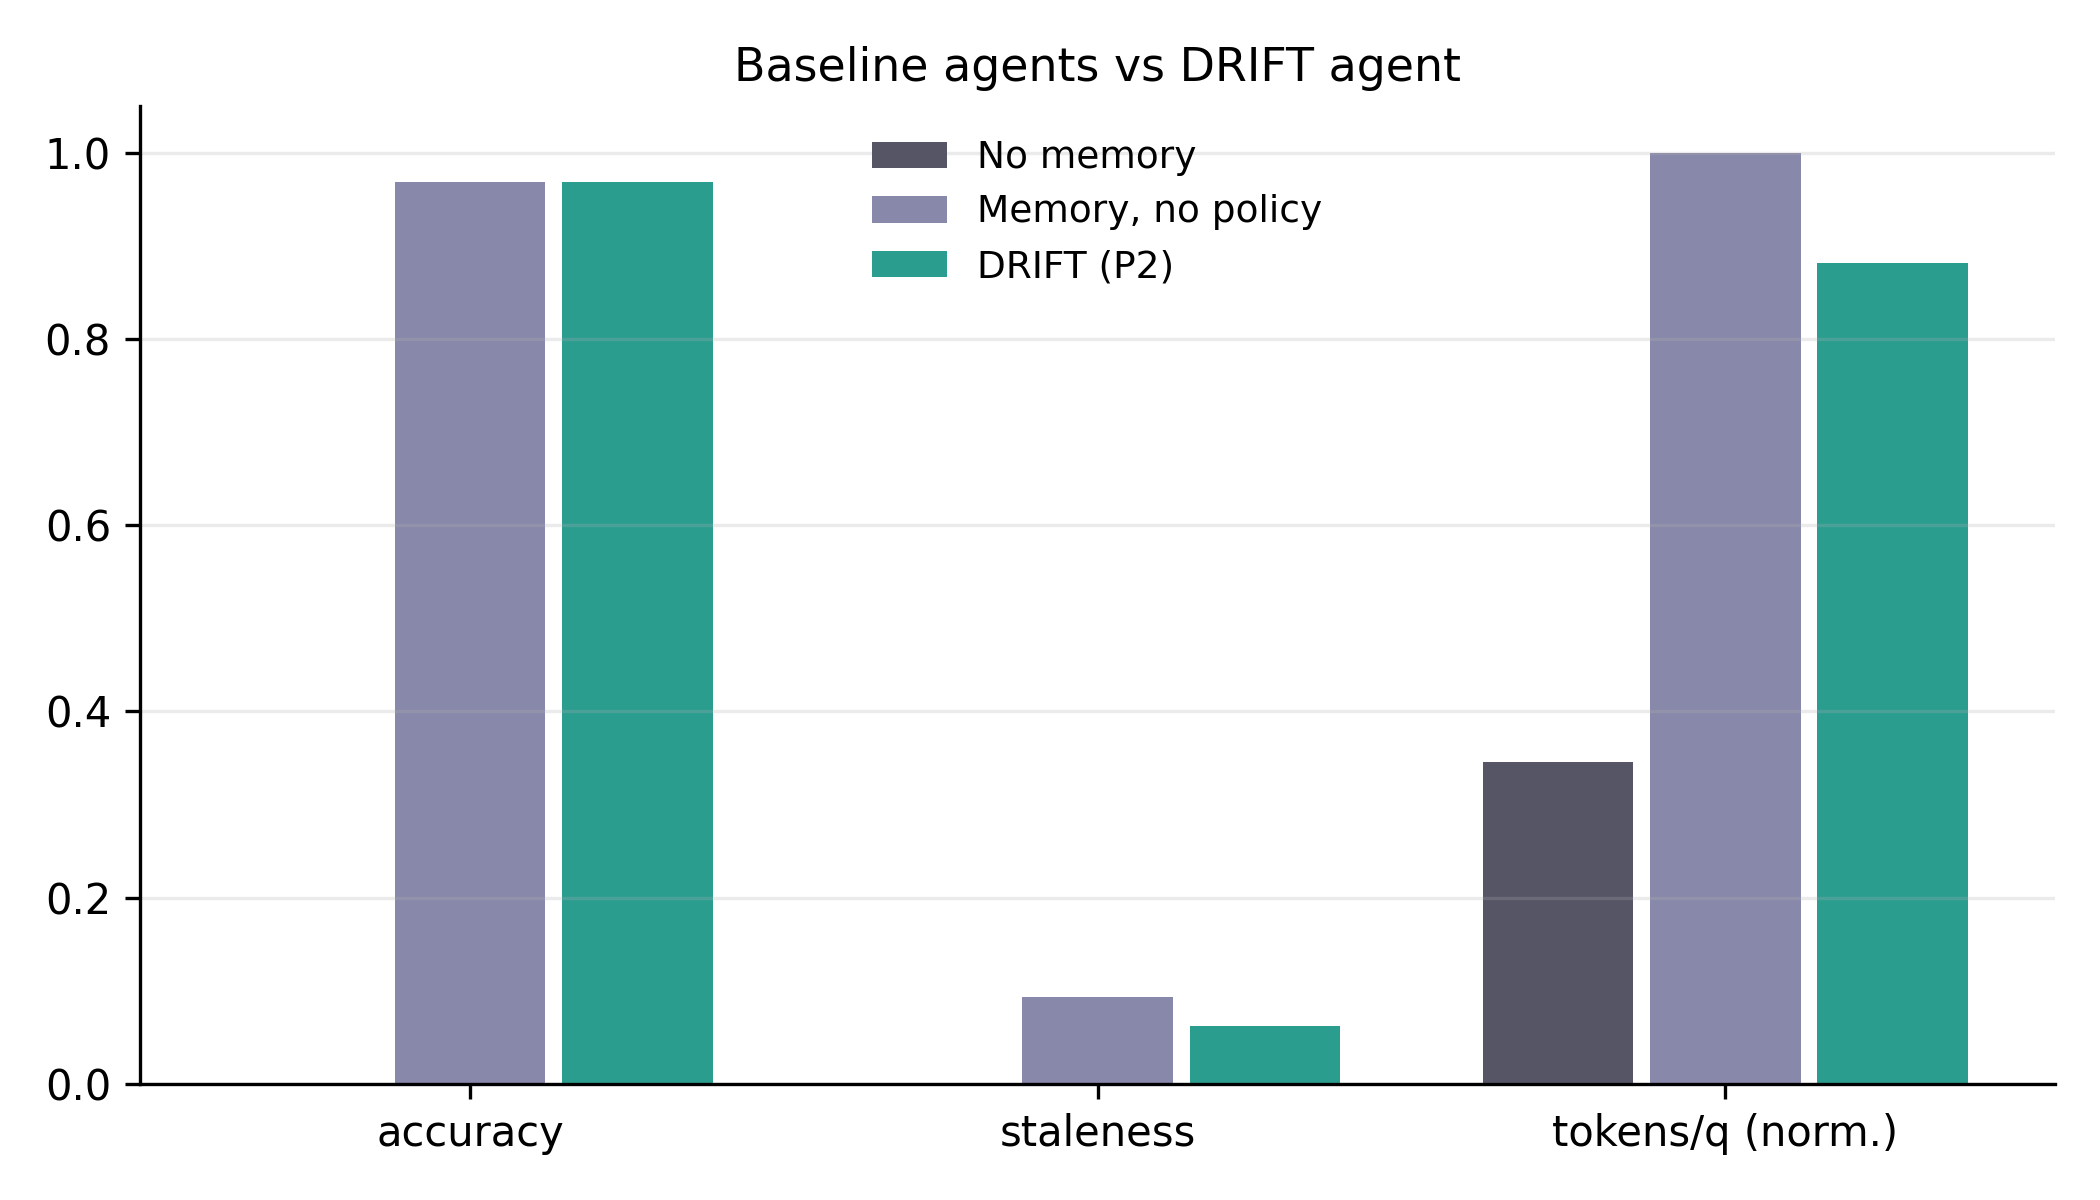
\includegraphics[width=0.75\textwidth]{figures/baseline_vs_drift_mquake_t.png}
\caption{The no-memory floor and the append-only ceiling plotted against the five forgetting policies, MQuAKE-T.}
\label{fig:baseline-vs-drift}
\end{figure}

\section{RQ2: Bitemporal Invalidation Is Free}
\label{sec:rq2}

\paragraph{Accuracy.} P2 matches P0 exactly on both benchmarks, at 0.840 against 0.840 on FactConsolidation and 0.969 against 0.969 on MQuAKE-T. The paired McNemar test returns 3 discordant pairs favoring each side on FactConsolidation ($p = 1.000$) and 2 discordant pairs favoring each side on MQuAKE-T ($p = 1.000$). The paired difference intervals reported in Table~\ref{tab:effect-sizes} bound the accuracy gap between P2 and P0 to within roughly $\pm 2.5$ percentage points on both benchmarks.

\paragraph{Cost.} Table~\ref{tab:cost-comparison} reports the token and memory-footprint savings P2 achieves relative to P0.

\begin{table}[H]
\centering
\caption{Cost comparison between P2 and the append-only ceiling P0.}
\label{tab:cost-comparison}
\begin{tabular}{lcccccc}
\toprule
Benchmark & P0 tok/q & P2 tok/q & Saved & P0 facts & P2 facts & Fewer \\
\midrule
FactConsolidation & 812 & 715 & 12.0\% & 380 & 324 & 14.7\% \\
MQuAKE-T & 816 & 716 & 12.2\% & 382 & 357 & 6.5\% \\
\bottomrule
\end{tabular}
\end{table}

The token saving replicates to within two tenths of a percentage point across two benchmarks of different provenance, which is a striking degree of consistency for an effect measured on independently constructed data. The memory-footprint saving differs more between the two benchmarks, which is itself expected behavior rather than a discrepancy to be explained away: P2 prunes exactly the facts that were superseded and have since aged past their grace period, and the two source corpora simply differ in what fraction of their facts meet that description.

\paragraph{No other policy achieves both properties simultaneously.} P1 stores substantially less memory than P0, at 210 and 251 facts against P0's 380 and 382, but loses 0.210 and 0.099 accuracy in exchange, a cost far larger than any saving P2 achieves. P3 and P5 shrink the memory footprint only modestly while losing accuracy and, as Sections~\ref{sec:novelty-gating-results} and~\ref{sec:rq3} show, gaining substantial staleness. P4 comes close to P2 on accuracy but saves essentially nothing on either token cost or memory footprint.

RQ2 is therefore answered directly: among the seven policies compared, P2 offers the best combined accuracy, staleness, and cost trade-off, and it does so by an equivalence margin on accuracy that is tight enough to be reported as a bound rather than as an inconclusive comparison.

\section{RQ3: Bitemporal Structure Beats Structure-Blind Structure}
\label{sec:rq3}

This section reports the ablation the experimental design exists specifically to support, and it produces the strongest result in this thesis.

P2 and P5 share the identical substrate, retrieval function, extraction step, answer model, and judge. Both are structure-aware, in the sense that both operate on the same knowledge graph and both perform a form of consolidation over it. The only difference between them is that P2 knows which of two competing facts is currently valid because it consults valid time directly, while P5 must infer which fact is current from structural corroboration count alone, having been deliberately denied access to valid time.

Table~\ref{tab:rq3-mquake} reports the comparison on MQuAKE-T, the benchmark where the effect is largest and where the mechanism is cleanest.

\begin{table}[H]
\centering
\caption{P2 versus P5 on MQuAKE-T.}
\label{tab:rq3-mquake}
\small
\begin{tabular}{p{2.6cm}ccp{2.7cm}cc}
\toprule
Metric & P2 & P5 & Paired delta & McNemar & $p$ \\
\midrule
Accuracy & 0.969 & 0.802 & +0.167 [+0.109, +0.224] & 34 to 2 & $< 0.001$ \\
Staleness & 0.036 & 0.214 & -0.177 [-0.240, -0.120] & 3 to 37 & $< 0.001$ \\
Retrieved-invalidated & 0.00 & 5.31 to 5.43 & & & \\
\bottomrule
\end{tabular}
\end{table}

P5's staleness is 5.9 times P2's staleness on this benchmark. Table~\ref{tab:rq3-failures} lists a representative sample of the questions where P5 returned the superseded value and P2 did not, chosen because each is independently verifiable against the public record as of the snapshot date used to construct the benchmark.

\begin{table}[H]
\centering
\caption{Representative questions where P5 answered from a superseded value that P2 correctly excluded.}
\label{tab:rq3-failures}
\small
\begin{tabular}{p{3.3cm}p{2.6cm}p{2.6cm}p{2.6cm}}
\toprule
Question & Gold (current as of snapshot) & P5 answered & P2 answered \\
\midrule
Head of state, South Korea & Yoon Suk-yeol & Moon Jae-in & Yoon Suk-yeol \\
Head of government, Czech Republic & Petr Fiala & Andrej Babi\v{s} & Petr Fiala \\
Head of state, Czech Republic & Petr Pavel & Milo\v{s} Zeman & Petr Pavel \\
Head of government, Malawi & Lazarus Chakwera & Peter Mutharika & Lazarus Chakwera \\
Head of state, Malawi & Lazarus Chakwera & Peter Mutharika & Lazarus Chakwera \\
Head of government, South Korea & Yoon Suk-yeol & Moon Jae-in & Yoon Suk-yeol \\
\bottomrule
\end{tabular}
\end{table}

\paragraph{The mechanism.} A long-serving predecessor accumulates more corroborating mentions throughout the memory graph simply by virtue of having been in office longer, and thus mentioned more often, than a recently installed successor. Corroboration-count consolidation therefore has a systematic bias toward preferring the outdated fact whenever tenure and recency are in tension. Recency alone is not a reliable proxy for correctness, since a fact can be recently observed and still wrong, but valid time specifically is a reliable proxy for currency, and that distinction between recency and validity is precisely what the bitemporal substrate encodes and what P5 has been deliberately denied.

\paragraph{Why the effect is sharper on MQuAKE-T than on FactConsolidation.} The same P2-versus-P5 comparison on FactConsolidation reaches $p = 0.022$ on accuracy and is inconclusive on staleness, at 3 to 5 discordant pairs with $p = 0.727$. FactConsolidation's entities are arbitrary Wikidata pairs whose corroboration is roughly uniform across the corpus, so P5's heuristic fails close to at random on that data, producing a small and comparatively noisy effect. MQuAKE-T's entities, by contrast, are real people holding real public offices, so corroboration in that corpus is systematically biased toward whoever has held the office of record for longer, and P5's heuristic therefore fails in a consistent, predictable direction rather than at random. The second benchmark did not merely replicate the finding observed on the first; it exposed the underlying mechanism in a way the first benchmark's more arbitrary entity structure could not.

RQ3 is therefore answered specifically: the advantage measured for bitemporal invalidation is attributable to bitemporal semantics themselves, and not merely to the more general property that the policy operates on graph structure. A structure-aware policy denied only temporal information performs significantly worse, at a magnitude and a level of statistical significance that leaves little room for an alternative explanation.

\section{Novelty Gating Causes Unrecoverable Staleness}
\label{sec:novelty-gating-results}

P3 exhibits 4.7 times P2's staleness on FactConsolidation, at 0.140 against 0.025, and 4.5 times P2's staleness on MQuAKE-T, at 0.161 against 0.036, both differences significant at $p < 0.001$, with paired deltas of $-0.115$ and $-0.125$ respectively.

\paragraph{The mechanism is structural, not statistical.} A fact update is, by construction, textually near-identical to the fact it supersedes, differing typically in only a single word or phrase:

\begin{quote}
\ttfamily
``Thomas Kyd was born in the city of London'' \quad (stored) \\
``Thomas Kyd was born in the city of Leeds'' \quad (the correction)
\end{quote}

A novelty gate computes the cosine similarity between an incoming candidate fact and its nearest neighbors already in memory. A correction of this kind registers as a near-duplicate of the fact it corrects, and the gate rejects the write. The correction never enters memory. No downstream mechanism, whether a smarter retrieval function, a reranking step, or a more careful prompt, can recover a value that was never stored in the first place, because the failure occurs at write time, before any of those downstream mechanisms have anything to operate on.

This mechanism was verified directly from saved knowledge-graph snapshots rather than merely hypothesized. On FactConsolidation, 46 write rejections produced 24 distinct subject-predicate pairs where P0's graph recorded the update correctly while P3's graph retained only the superseded value. On MQuAKE-T, 31 write rejections produced 14 questions that P3 answered from a stale value that P0 answered correctly. Table~\ref{tab:novelty-failures} lists a representative sample.

\begin{table}[H]
\centering
\caption{Representative questions where P3's novelty gate rejected the correcting fact.}
\label{tab:novelty-failures}
\small
\begin{tabular}{p{4.2cm}p{3.2cm}p{3.2cm}}
\toprule
Question & Gold & P3 retained \\
\midrule
Head of state, United Kingdom & Charles, Prince of Wales & Elizabeth II \\
Head of state, South Korea & Yoon Suk-yeol & Moon Jae-in \\
Headquarters city, Scientific American & Los Angeles & New York City \\
Head of state, Mongolia & Khurelsukh Ukhnaa & Khaltmaagiin Battulga \\
Headquarters city, Apax Partners & Paris & London \\
\bottomrule
\end{tabular}
\end{table}

This is, of the results in this thesis, the most transferable to other systems, because it follows directly from the definition of a novelty gate and from the textual form a correction necessarily takes, rather than from any detail specific to this thesis's implementation of one. The precise rate at which the failure occurs will differ across corpora with different rates of factual correction, but the failure mode itself will not, and any workload in which facts are corrected over time inherits it by construction.

The asymmetry between the saving and the liability is what makes this failure mode serious rather than merely a curiosity. The saving in memory footprint is bounded: P3 retained 334 and 351 facts against P0's 380 and 382, a reduction of 12 percent and 8 percent respectively. The liability, in contrast, is unbounded: once a correction is rejected, the wrong value persists in memory indefinitely, and it cannot be corrected by any later mechanism, because as far as the substrate is concerned, the correction was never offered.

\section{Generalization Across Benchmarks}
\label{sec:generalization}

Spearman's rank correlation on the policy ranking across the two benchmarks is 0.891, computed over all seven policies. Table~\ref{tab:generalization} shows the ranking on each benchmark side by side.

\begin{table}[H]
\centering
\caption{Policy ranking on each benchmark, by accuracy.}
\label{tab:generalization}
\begin{tabular}{lccl}
\toprule
Policy & FC rank & MQ rank & Stable \\
\midrule
P0 & 1 & 1 & yes \\
P2 & 2 & 2 & yes \\
P4 & 3 & 3 & yes \\
P5 & 4 & 5 & no \\
P3 & 5 & 6 & no \\
P1 & 6 & 4 & no, moves two places \\
NOMEM & 7 & 7 & yes \\
\bottomrule
\end{tabular}
\end{table}

The most informative row in this table is P1's. On MQuAKE-T, every question by construction concerns a fact that has changed, so the gold answer is always the recent value, and time-based pruning removes mostly facts that have genuinely been superseded, which is largely harmless. On FactConsolidation, only 65 percent of questions concern a fact that has changed, so time-based pruning also removes a substantial number of stable, still-answerable facts, which is directly destructive to accuracy. P1's rank, in other words, is a property of how much of the target workload consists of updates, rather than an intrinsic property of time-based pruning as a strategy.

The top and the bottom of the ranking are stable across both benchmarks; the middle of the ranking is workload-dependent. This should not be read as a weakness of the study. It is the study's own central argument, demonstrated directly: which forgetting policy is best is an empirical question about the target workload rather than a question with a universal answer, and P1 shifting by two ranking places when the fraction of update-relevant questions changes is the clearest available demonstration of that argument within the data collected for this thesis.

\section{Ablation: How Much of the Result Is a Configuration Choice?}
\label{sec:ablation}

The \texttt{functional\_predicates} setting declares to the substrate which predicates in a given domain admit only a single true object at a time, which is the information contradiction detection relies on. FactConsolidation required this setting to be configured as ``all predicates,'' a choice made while directly inspecting that dataset, which makes it the single largest threat to the external validity of the results in this thesis. To quantify the consequence of this choice, MQuAKE-T was rerun with the setting left at the substrate's built-in default, a set of predicates drawn from personal-conversation contexts that happens to cover none of MQuAKE-T's actual relations. Under this default, invalidations in the graph drop from 59 to 1, which effectively switches P2's contradiction-detection mechanism off.

\begin{table}[H]
\centering
\caption{Effect of declaring \texttt{functional\_predicates} on MQuAKE-T.}
\label{tab:ablation}
\small
\begin{tabular}{p{3.4cm}cp{2.6cm}l}
\toprule
Cell & Declared & Not declared & Change \\
\midrule
P2 accuracy & 0.969 & 0.969 & none \\
P2 tokens per question & 641 & 733 & $+14.4\%$ \\
P2 active facts & 357 & 382 & $+7.0\%$ \\
P2 retrieved-invalidated & 0.00 & 0.00 & none \\
P0 accuracy & 0.969 & 0.969 (corrected, see Section~\ref{sec:judge-audit}) & none \\
P3 accuracy & 0.802 & 0.802 & none, as expected \\
Graph invalidations & 59 & 1 & mechanism off \\
\bottomrule
\end{tabular}
\end{table}

The declaration buys P2 none of its accuracy and all of its efficiency. This is a more precise and more useful result than either of the two simpler alternatives, that the setting matters or that it does not. It decomposes P2's overall benefit into two separable parts: P2 is safe to enable without tuning, because an incorrectly configured P2 degrades gracefully to the behavior of append-only memory rather than to something worse, but P2 only pays for itself, in the sense of reducing token cost and memory footprint, when the domain's functional predicates have actually been declared. That is a specific, actionable deployment instruction derived directly from measurement rather than from intuition.

\section{A Judge-Reliability Audit}
\label{sec:judge-audit}

While reconciling the ablation run described in Section~\ref{sec:ablation} against the main MQuAKE-T run, the ablation's P0 cell was found to have produced 96 of 96 byte-identical answers to the main run's P0 cell, and yet was scored 0.844 against the main run's 0.969. Twelve verdicts flipped between the two runs, all in the same direction, on answers of the following character:

\begin{quote}
\small\ttfamily
Question: What is the name of the current head of \\
\quad the Australia government? \\
Gold: Anthony Albanese \\
Answer: Anthony Albanese \quad (judged INCORRECT)
\end{quote}

To quantify how often this occurs, every experimental cell was audited for answers whose normalized form contains the gold answer verbatim and yet were graded incorrect by the judge. Table~\ref{tab:judge-audit} reports the result.

\begin{table}[H]
\centering
\caption{Audit of verbatim-correct answers graded incorrect.}
\label{tab:judge-audit}
\small
\begin{tabular}{p{4.3cm}p{2.6cm}p{2cm}c}
\toprule
Scope & Verbatim-correct answers & Judged incorrect & Rate \\
\midrule
FactConsolidation, all cells & 515 & 3 & 0.6\% \\
MQuAKE-T, all cells & 782 & 12 & 1.5\% \\
MQuAKE-T ablation, P0 cell alone & 93 & 14 & 15.1\% \\
\bottomrule
\end{tabular}
\end{table}

The baseline judge false-negative rate across the full campaign is roughly 1 to 2 percent, which is small enough that it does not change any conclusion reported elsewhere in this thesis. One specific cell, however, happened to draw a comparatively unreliable member of the three-provider judge fallback pool and lost 12.5 accuracy points on answers that were, by direct string comparison, correct. The ablation's reported P0 accuracy of 0.844 is therefore an artifact of judge assignment rather than a property of the policy; the true value, reported in Section~\ref{sec:ablation} and Table~\ref{tab:ablation}, is 0.969.

Three consequences follow from this audit.

\begin{enumerate}
\item Any reported gap between two policies smaller than roughly three percentage points should be treated as inside the noise floor established by this audit and not treated as interpretable evidence of a genuine difference. This places the comparison between P2 and P4 on MQuAKE-T, with a delta of $+0.016$ and $p = 0.549$, outside the range this thesis is willing to interpret, while leaving the results reported in Sections~\ref{sec:rq3} and~\ref{sec:novelty-gating-results}, at 16.7 and 17.7 points respectively with $p < 0.001$ in both cases, far outside the noise floor and therefore fully interpretable.
\item Judge rotation across a fallback pool is simultaneously a resilience mechanism and a confound. The pool exists precisely so that one provider running out of quota does not terminate an entire campaign, but its existence also means two experimental cells can, in principle, be graded by two different underlying judge models without that fact being visible in the summary statistics. The practical recommendation is to pin a single judge for any run whose numbers will be reported, or, at minimum, to record which judge model graded each individual record so that this kind of artifact is auditable after the fact rather than requiring archaeology to uncover.
\item The verbatim-match audit performed here is inexpensive, requiring on the order of ten lines of code, and it caught a 12.5-point artifact that would otherwise very plausibly have been written up as a genuine policy effect.
\end{enumerate}

This audit is reported here in full, including the specific cell in which the artifact occurred, because it is a class of error that is easy to commit and correspondingly hard to detect from summary statistics alone, and because the practice of using a language model as a judge is now standard across this subfield of research.

\section{RQ4: Multi-Agent Topologies}
\label{sec:rq4}

The multi-agent harness built for this thesis runs the same seven policies across three topologies, all operating over the same substrate and the same policy implementations used in the single-agent experiments. Table~\ref{tab:topologies} describes the three topologies.

\begin{table}[H]
\centering
\caption{The three multi-agent topologies evaluated.}
\label{tab:topologies}
\small
\begin{tabular}{lp{5.3cm}p{5.3cm}}
\toprule
Topology & Structure & What it isolates \\
\midrule
Shared & Five writer agents round-robin into one shared graph, each fact tagged with the identity of the agent that wrote it & Write contention: a contradiction can now arrive from a different agent than the one that wrote the original fact \\
Independent & Five agents, each with a private graph, each seeing a seeded random 80 percent of sessions & Robustness under partial observation of the underlying data \\
Orchestrator & One shared graph, with a router language model assigning each incoming question to one of five specialist worker agents & The production coordinator-worker pattern, in which the agent that reads a fact is not the agent that wrote it \\
\bottomrule
\end{tabular}
\end{table}

Table~\ref{tab:swarm-results} reports results on synthetic data using the offline mock provider, with 14 questions per cell.

\begin{table}[H]
\centering
\caption{Accuracy and staleness by policy across the three topologies, offline synthetic data. Cells are accuracy / staleness.}
\label{tab:swarm-results}
\small
\begin{tabular}{lccccc}
\toprule
Policy & Shared & Independent & Orchestrator & Cross-writer inval. \\
\midrule
NOMEM & 0.000 / 0.000 & 0.000 / 0.000 & 0.000 / 0.000 & 5 \\
P0 & 0.714 / 0.286 & 0.667 / 0.286 & 0.714 / 0.286 & 5 \\
P1 (TTL 14d) & 0.143 / 0.000 & 0.143 / 0.000 & 0.143 / 0.000 & 3 \\
\textbf{P2} & \textbf{0.929} / \textbf{0.000} & \textbf{0.881} / \textbf{0.000} & \textbf{0.929} / \textbf{0.000} & 5 \\
P3 & 0.714 / 0.286 & 0.667 / 0.286 & 0.714 / 0.286 & 5 \\
P4 & 0.714 / 0.286 & 0.667 / 0.286 & 0.714 / 0.286 & 5 \\
P5 & 0.500 / 0.143 & 0.548 / 0.095 & 0.500 / 0.071 & 4 \\
\bottomrule
\end{tabular}
\end{table}

P2 leads all seven policies in all three topologies and holds staleness at exactly 0.000 in all three. Every shared-topology invalidation observed arrives cross-writer, meaning the fact that closed a validity window was written by a different agent than the one that wrote the original fact, which is direct evidence that structure-aware forgetting of this kind is writer-agnostic by construction rather than by any special-case handling.

This result should be read as validation of the multi-agent harness rather than as a settled finding. The sample size is 14 questions using a deterministic mock provider rather than a real language model, and it covers the full seven-policy, three-topology design without yet answering whether that design holds under real, heterogeneous multi-model extraction. Section~\ref{sec:rq4-pilot} reports a partial real-data pilot that probes exactly this question on one topology, and finds a real boundary condition. Of the four research questions posed in Chapter~\ref{chap:introduction}, RQ4 remains the one with the weakest evidentiary support, and Chapter~\ref{chap:discussion} discusses completing it as the highest-priority item of future work.

\begin{figure}[H]
\centering
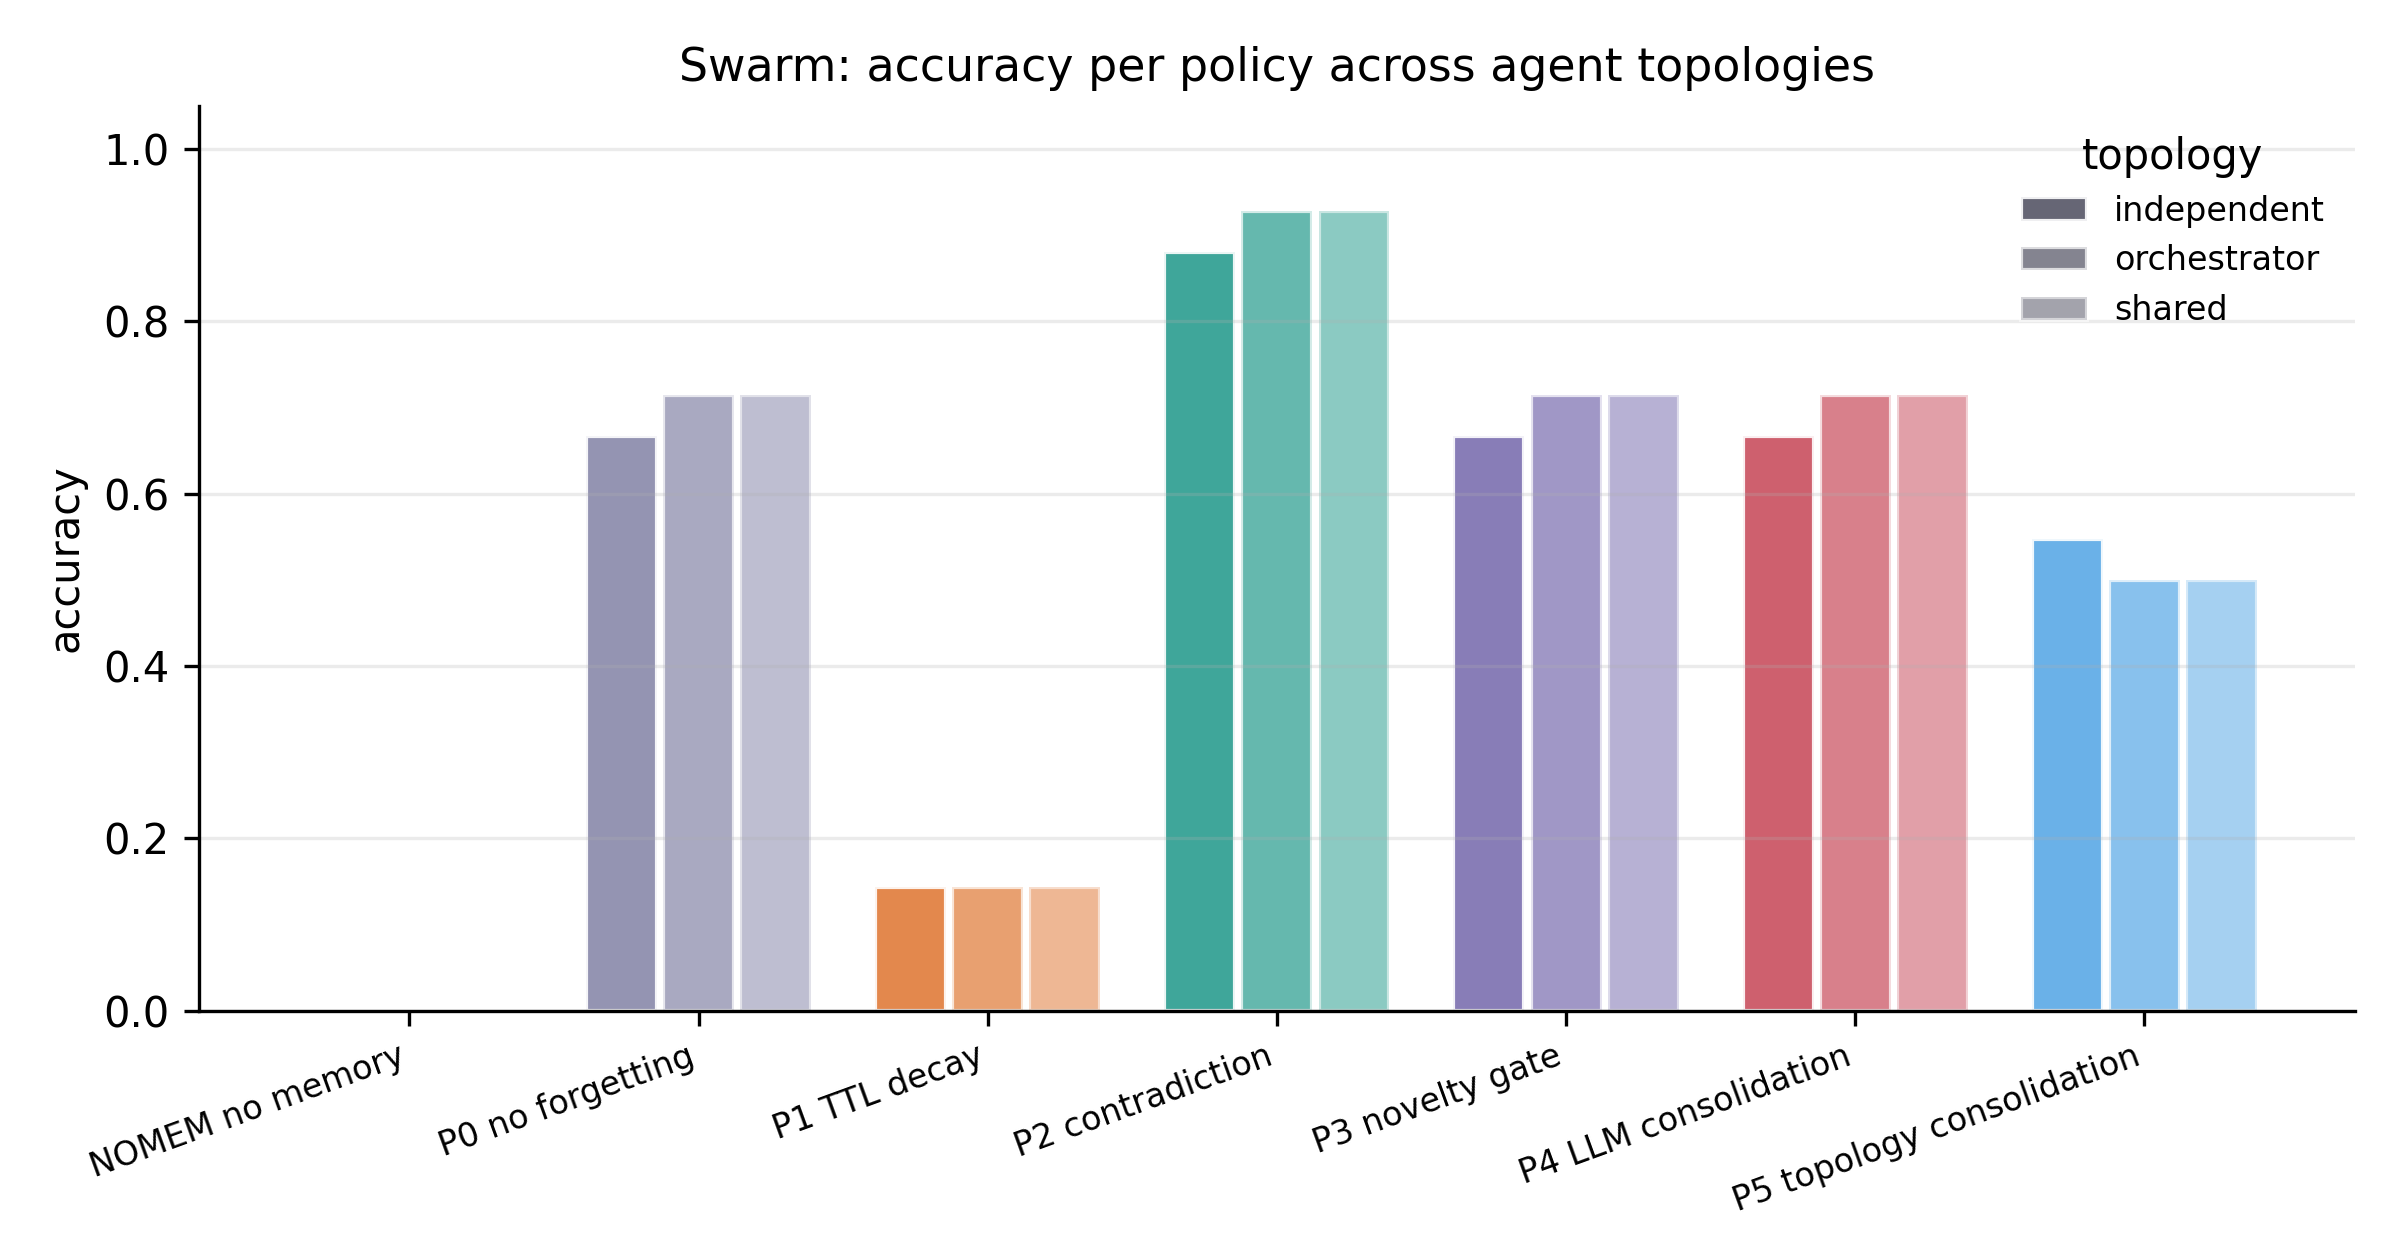
\includegraphics[width=0.8\textwidth]{figures/swarm_topology.png}
\caption{Accuracy and staleness by policy across the three multi-agent topologies.}
\label{fig:swarm-topology}
\end{figure}

\begin{figure}[H]
\centering
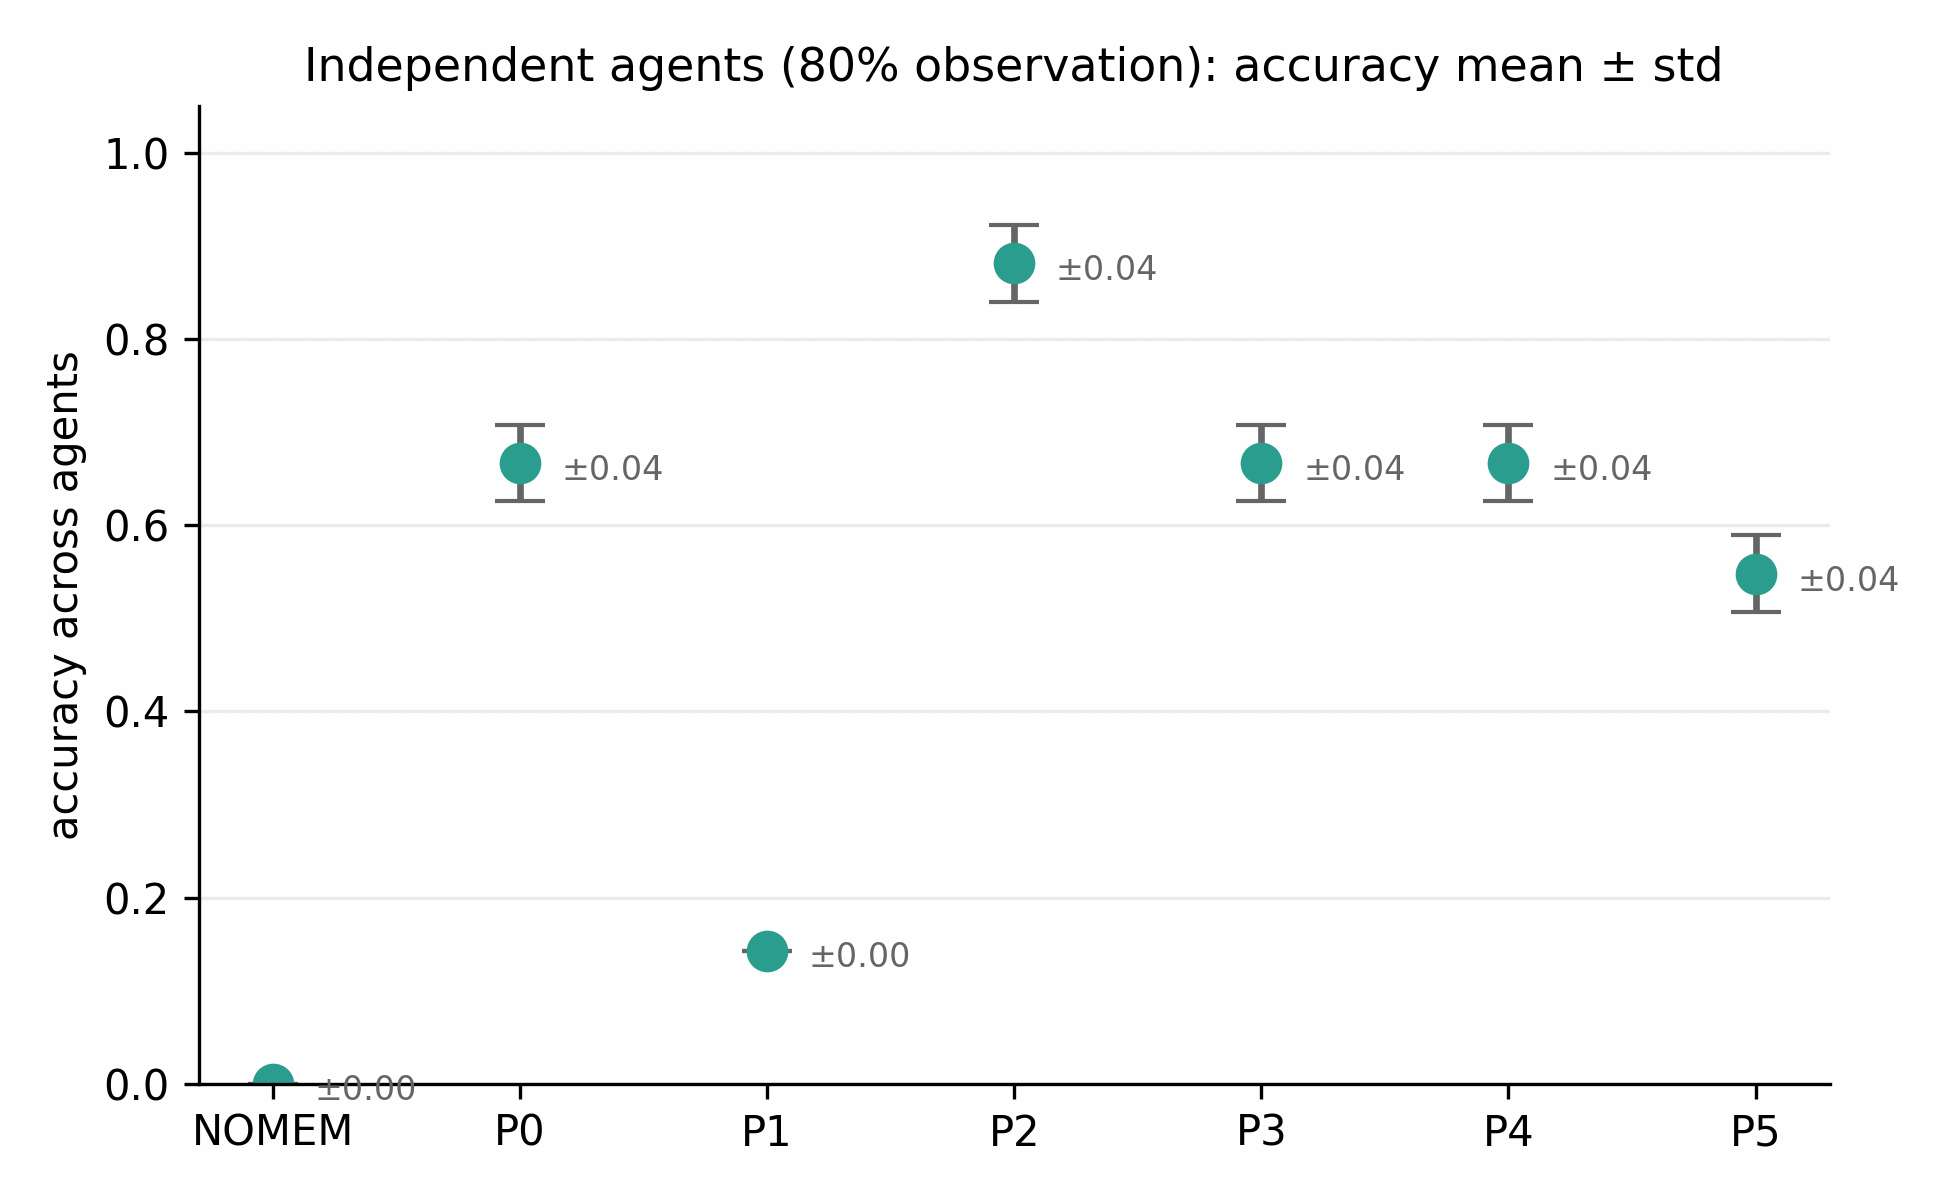
\includegraphics[width=0.7\textwidth]{figures/swarm_variance.png}
\caption{Mean and standard deviation of accuracy across the five independent agents in the independent topology.}
\label{fig:swarm-variance}
\end{figure}

\subsection{A Real-Data Pilot on the Shared Topology}
\label{sec:rq4-pilot}

A partial real-data campaign was run on the shared topology using MQuAKE-T and five heterogeneous extraction models, one per writer agent: GLM-5.2, MiniMax-M3, Gemini-3.1-Flash-Lite, Nemotron-3-Ultra, and Hunyuan, with GLM-5.2 as the shared answer model. Owing to the wall-clock cost of the P4 and P5 policies at this sample size, the pilot covers five of seven policies (NOMEM, P0, P1, P2, P3) on one of three topologies rather than the full matrix. Table~\ref{tab:rq4-pilot} reports the results.

\begin{table}[H]
\centering
\caption{Real-data pilot, shared topology, MQuAKE-T, 96 questions, five heterogeneous extraction models.}
\label{tab:rq4-pilot}
\small
\begin{tabular}{lccccc}
\toprule
Policy & Accuracy & Staleness & Tok/q & Invalidations & Active facts \\
\midrule
NOMEM & 0.000 & 0.000 & 156 & 0 & 140 \\
P0 & 0.333 & 0.271 & 710 & 0 & 140 \\
P1 (TTL 20d) & 0.281 & 0.135 & 729 & 0 & 79 \\
P2 & 0.365 & 0.271 & 710 & 0 & 140 \\
P3 & 0.365 & 0.271 & 710 & 0 & 140 \\
\bottomrule
\end{tabular}
\end{table}

The invalidation column is the finding. In the single-agent runs, one consistent extraction model per cell, P2 closes dozens of valid-time windows on MQuAKE-T (Section~\ref{sec:rq1}). Here, with five different models extracting from the same sessions, P2 records zero invalidations, and its retained-fact count, 140 active and 0 pruned, is identical to P0's. P2 and P3 track P0 to within 3.2 accuracy points, a gap the judge-reliability audit in Section~\ref{sec:judge-audit} already established as inside single-provider judge noise at this sample size, so the honest reading is that all three are statistically indistinguishable in this cell: bitemporal invalidation did not engage.

The mechanism is visible directly in the saved graph. Of 140 stored facts spanning 30 distinct predicate strings, the same underlying relation is extracted under multiple surface forms depending on which model wrote it: \texttt{head\_of\_government} (28 occurrences), \texttt{is\_head\_of\_government\_of} (9), and \texttt{head\_of\_government\_of} (7) all co-occur for what MQuAKE-T's schema treats as one functional predicate, and the same pattern appears on \texttt{citizen\_of} (32) versus \texttt{is\_citizen\_of} (6) versus \texttt{citizenship} (5). P2's contradiction detection matches on subject and predicate string; a correction extracted under a different surface form than the fact it corrects never triggers a match, so the valid-time window never closes. Only 3 of 137 subjects in the graph carry more than one fact at all, each exactly 2, versus the dozens of multi-fact subjects typical of the single-extractor single-agent runs, consistent with the same real-world relation being scattered across string variants rather than consolidated onto one.

P1 is the one policy in this pilot whose staleness reduction survives extraction heterogeneity, 0.135 versus P0's 0.271, because time-to-live pruning keys on \texttt{t\_valid\_start} alone and never needs two facts to agree on a predicate string to act. That protection is not free: P1 also prunes facts that were never superseded, and its accuracy, 0.281, is the lowest of the four non-floor policies in this pilot.

This pilot does not overturn the single-agent findings above; it identifies a boundary condition on them. P2's advantage over P0 was established, and holds, when one extractor is responsible for the graph's predicate vocabulary. It is not yet established for the heterogeneous-extractor case this pilot probes, and the mechanism above, predicate-string fragmentation defeating exact-match contradiction detection, is a directly observed explanation rather than a speculative one. A canonicalization step ahead of the write-time match, mapping extracted predicate strings to a fixed schema or matching on embedding similarity rather than string equality, is the natural fix and is noted as future work in Chapter~\ref{chap:discussion}. The remaining sixteen cells of the full twenty-one-cell matrix, both remaining topologies plus P4 and P5 on the shared topology, were not completed in the time available for this thesis; Table~\ref{tab:swarm-results} above remains the only evidence on the full seven-policy, three-topology design, and it is offline-synthetic.

\section{Memory Growth}
\label{sec:memory-growth}

Table~\ref{tab:memory-growth} reports the count of active facts in memory at five checkpoints across the 38 sessions of each benchmark, using the GLM-5.2 answer model.

\begin{table}[H]
\centering
\caption{Active fact count at session checkpoints.}
\label{tab:memory-growth}
\begin{tabular}{lccccc}
\toprule
& \multicolumn{5}{c}{FactConsolidation} \\
Policy & s1 & s10 & s20 & s30 & s38 \\
\midrule
P0 & 10 & 100 & 200 & 300 & 380 \\
P1 & 10 & 100 & 200 & 210 & 210 \\
P2 & 10 & 100 & 189 & 270 & 324 \\
P3 & 10 & 98 & 185 & 273 & 334 \\
P4 & 10 & 96 & 195 & 294 & 374 \\
P5 & 10 & 100 & 198 & 291 & 365 \\
\midrule
& \multicolumn{5}{c}{MQuAKE-T} \\
Policy & s1 & s10 & s20 & s30 & s38 \\
\midrule
P0 & 1 & 74 & 169 & 276 & 382 \\
P1 & 1 & 74 & 169 & 209 & 251 \\
P2 & 1 & 74 & 165 & 266 & 357 \\
P3 & 1 & 74 & 164 & 264 & 351 \\
P4 & 1 & 74 & 166 & 266 & 369 \\
P5 & 1 & 74 & 168 & 271 & 365 \\
\bottomrule
\end{tabular}
\end{table}

Two observations follow from this table. P1's curve flattens abruptly once its time-to-live horizon is reached, which is the direct cause of its accuracy collapse reported in Section~\ref{sec:headline}: it is discarding answerable facts wholesale once they cross the age threshold, rather than selectively discarding only facts that have actually been superseded. P2's curve, by contrast, tracks P0's closely for most of the run and diverges only gradually, which is exactly the shape one would expect from a policy that removes only what has genuinely become invalid rather than removing by a blunt criterion such as age.

\begin{figure}[H]
\centering
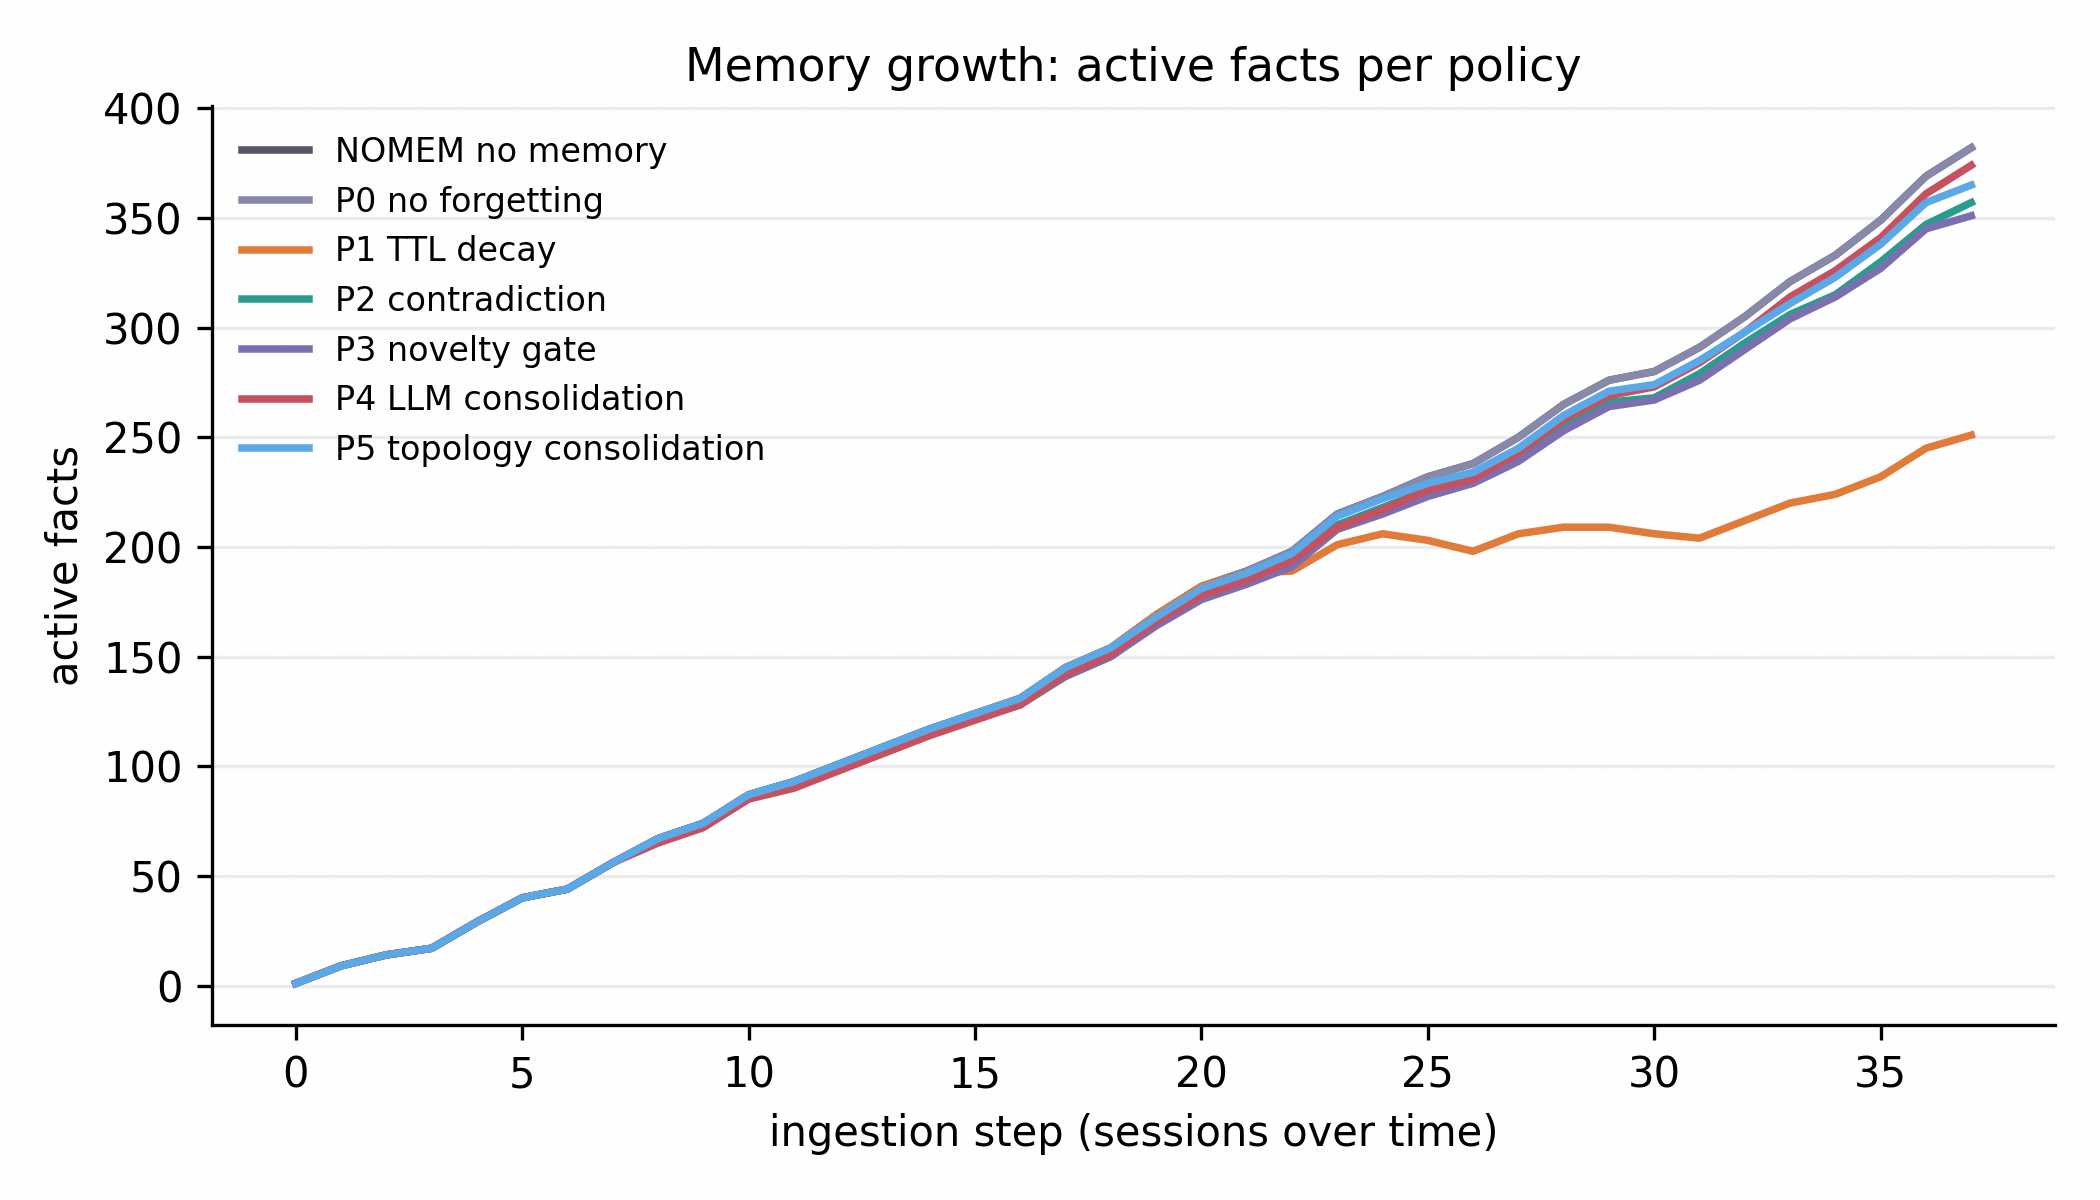
\includegraphics[width=0.75\textwidth]{figures/memory_growth_mquake_t.png}
\caption{Active fact count over the course of the 38 MQuAKE-T sessions, by policy.}
\label{fig:memory-growth}
\end{figure}

\section{Per-Model Breakdown}
\label{sec:per-model}

Table~\ref{tab:per-model} reports accuracy broken out by the two answer models used in this thesis, GLM-5.2 and MiniMax-M3, to check whether the policy effects reported above are an idiosyncrasy of a single answer model.

\begin{table}[H]
\centering
\caption{Accuracy by policy, broken out by answer model.}
\label{tab:per-model}
\begin{tabular}{lcccc}
\toprule
Policy & FC GLM-5.2 & FC MiniMax-M3 & MQ GLM-5.2 & MQ MiniMax-M3 \\
\midrule
NOMEM & 0.000 & 0.000 & 0.000 & 0.000 \\
P0 & 0.860 & 0.820 & 0.969 & 0.969 \\
P1 & 0.650 & 0.610 & 0.865 & 0.875 \\
P2 & 0.850 & 0.830 & 0.969 & 0.969 \\
P3 & 0.680 & 0.650 & 0.802 & 0.781 \\
P4 & 0.820 & 0.780 & 0.958 & 0.948 \\
P5 & 0.820 & 0.770 & 0.823 & 0.781 \\
\bottomrule
\end{tabular}
\end{table}

\begin{figure}[H]
\centering
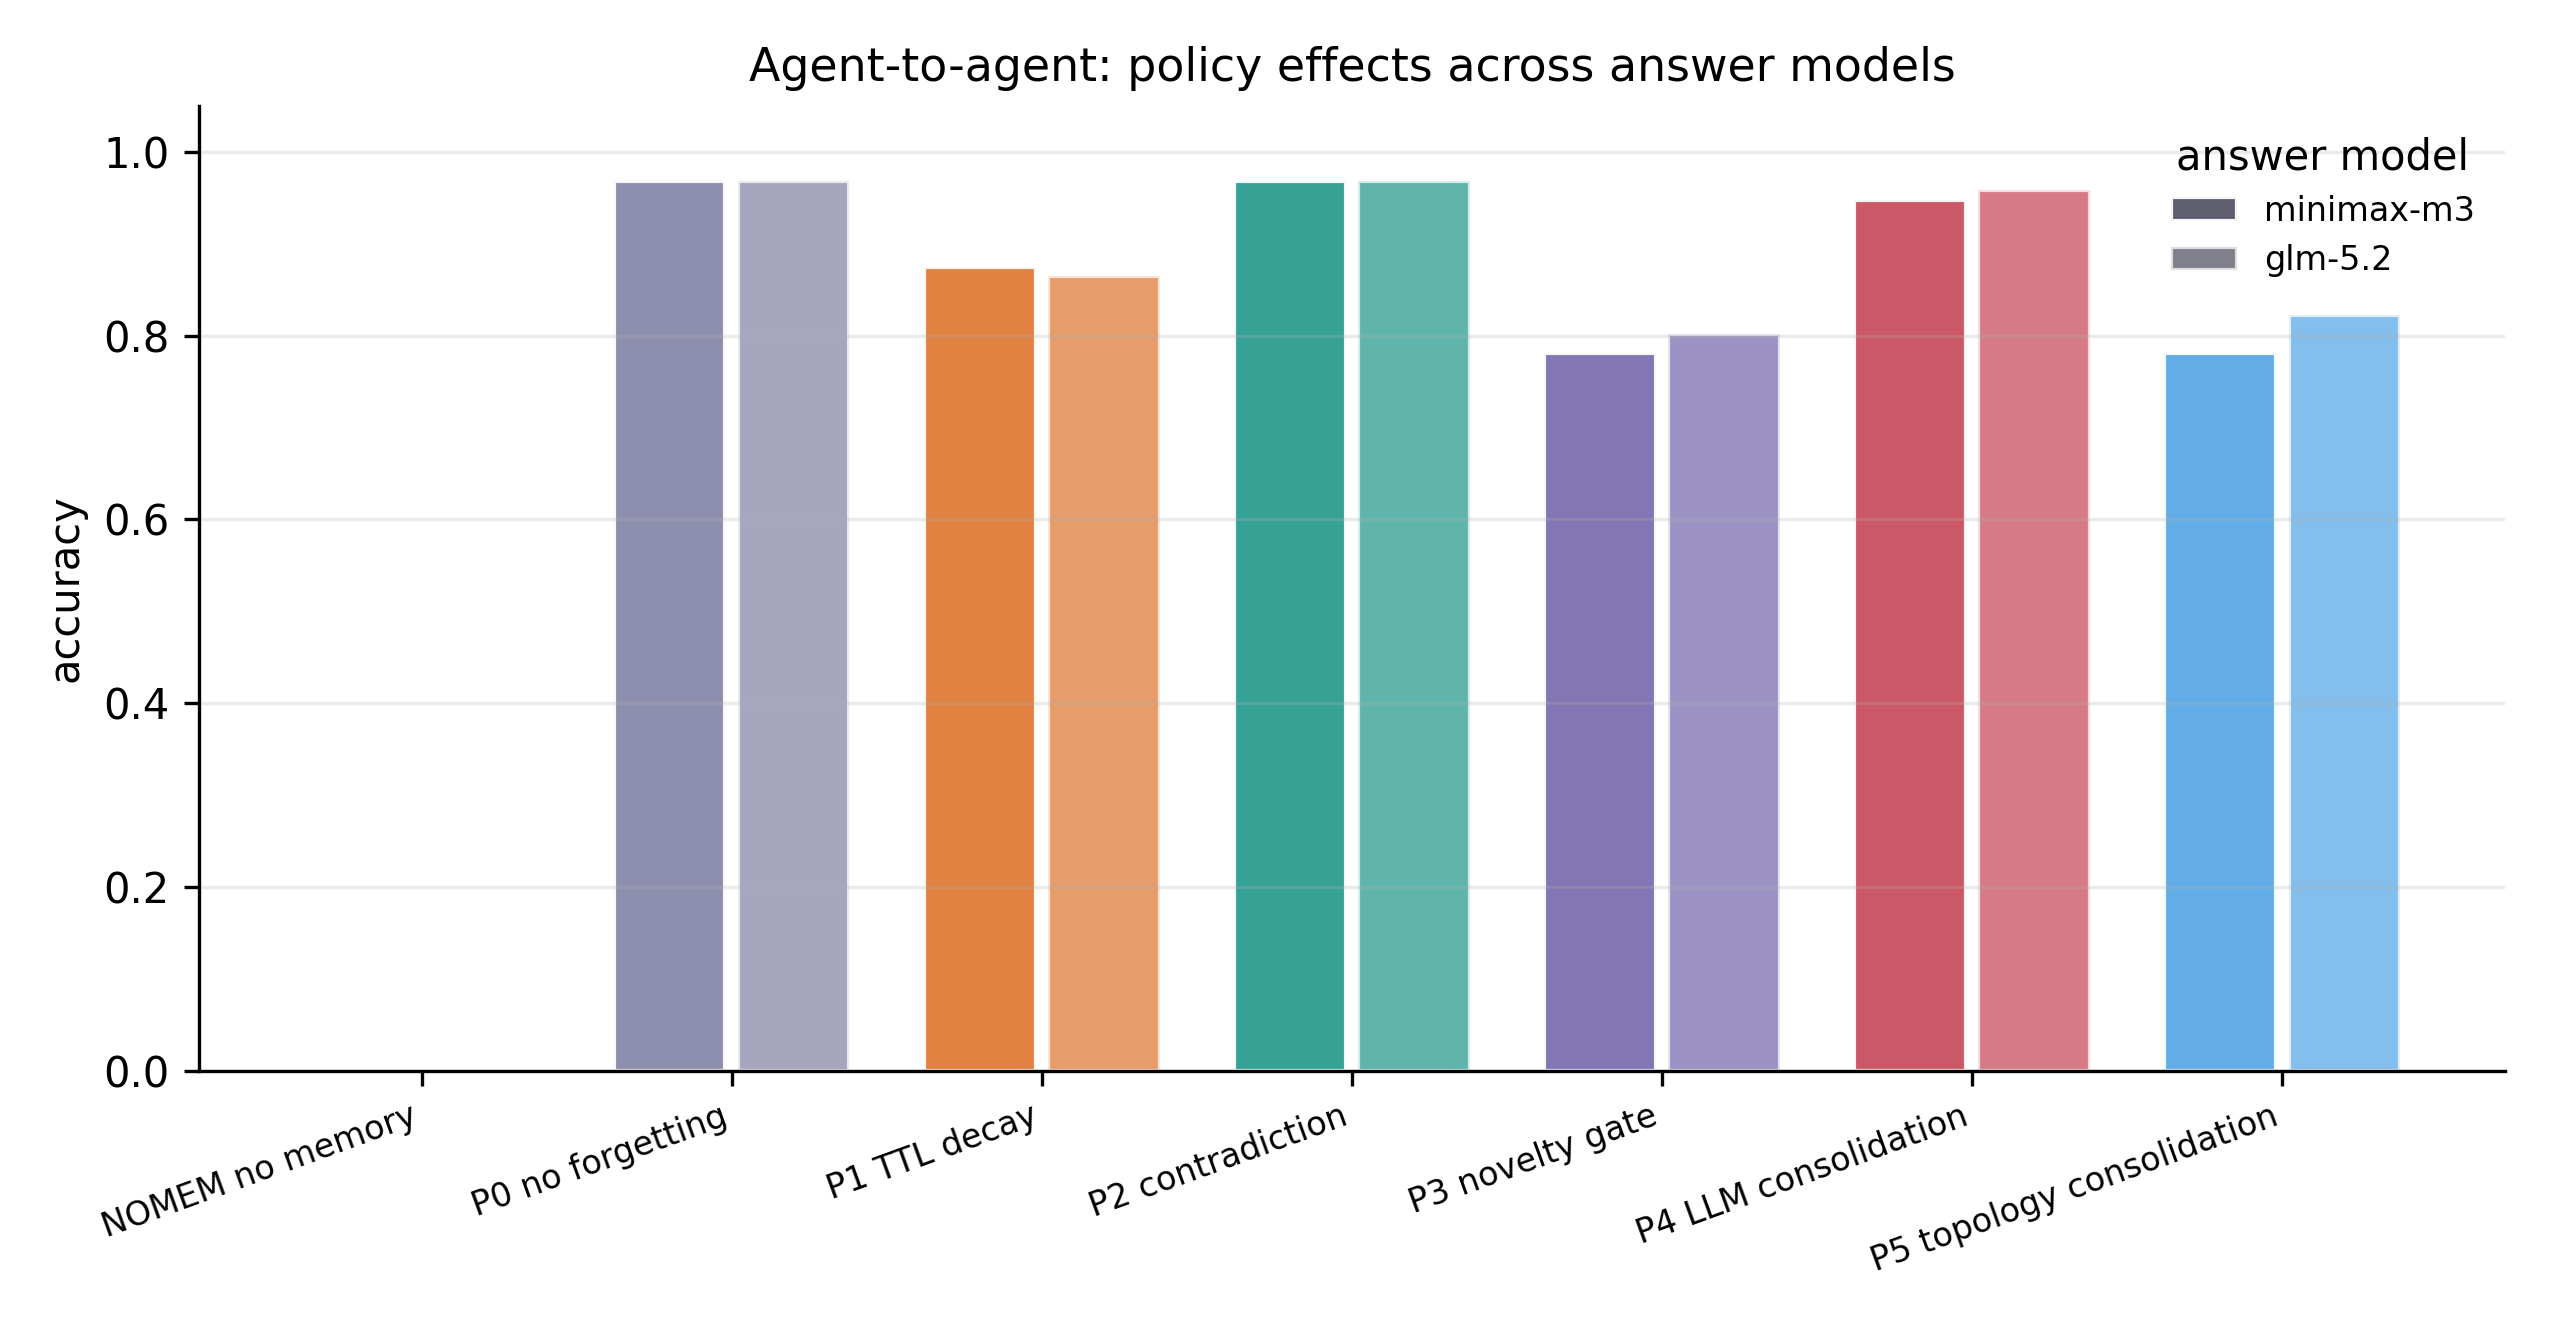
\includegraphics[width=0.75\textwidth]{figures/model_comparison_mquake_t.png}
\caption{Accuracy by policy, broken out by answer model, MQuAKE-T.}
\label{fig:model-comparison}
\end{figure}

Both answer models rank all seven policies in the identical order. Token-F1, not shown in this table, diverges sharply between the two models, for example 0.973 against 0.622 for P0 on MQuAKE-T, because MiniMax-M3 tends to answer more verbosely and token-F1 penalizes length directly. Accuracy, which is scored semantically by a judge rather than by lexical overlap, agrees closely between the two models despite this divergence in verbosity. This is itself a small methodological observation worth stating explicitly: token-F1 should not be relied upon as a primary metric when comparing models with substantially different verbosity profiles, precisely because it can disagree with a semantic judgment for reasons unrelated to correctness.
   % Results
\chapter{Discussion and Conclusion}
\label{chap:discussion}

This chapter interprets the results reported in Chapter~\ref{chap:results}, discusses their significance for research and for practice, situates the DRIFT framework as an artifact going forward, states the threats to the validity of the conclusions in full, describes the limitations of the study and the work they motivate, and closes with a summary conclusion.

\section{Why the Results Come Out This Way}
\label{sec:why-results}

\subsection{Why Forgetting Can Be Free}
\label{sec:why-forgetting-free}

The common intuition that forgetting must cost accuracy rests on an implicit assumption: that all stored information has non-negative expected value at the moment it might be retrieved. Bitemporal invalidation violates that assumption in a specific and identifiable way. It removes only facts whose valid-time window has been closed, meaning facts that a later observation has explicitly contradicted. Such facts have negative expected value at retrieval time, because surfacing them to the answer model can only produce a stale answer; there is no scenario under this policy's design in which retrieving an invalidated fact helps.

This explains the shape of the result reported in Section~\ref{sec:rq2}. P2 does not trade accuracy for efficiency in the way a naive intuition might predict. It removes information that was already harmful to retrieve, so the efficiency gain arrives without a corresponding accuracy cost, and the paired bootstrap interval bounding the P2-versus-P0 accuracy gap to within roughly two and a half points is the quantitative expression of that fact. Time-to-live decay, policy P1, removes facts by age instead, a criterion that is uncorrelated with whether a fact has actually been superseded. It therefore destroys useful and harmful information indiscriminately, and it pays for whatever memory savings it achieves in a substantial loss of accuracy, as Section~\ref{sec:headline} reports.

The general principle this result supports is that a forgetting policy is free, in the sense of costing nothing in accuracy, exactly to the extent that its removal criterion correlates with the harmfulness of the information being removed, rather than with the information's age or its textual redundancy relative to other stored facts.

\subsection{Why Novelty Gating Fails, Structurally}
\label{sec:why-novelty-fails}

A novelty gate makes an inference from textual similarity to informational redundancy: if a candidate fact looks like something already in memory, the gate infers that storing it adds nothing new. That inference is sound for genuine duplicates, restatements of a fact that add no new information, but it fails precisely for corrections, because a correction is, almost by definition, a minimal edit of the thing it corrects. The gate's discriminative signal, textual similarity, is inversely aligned with exactly the case that matters most for an agent that needs to stay current: the case in which a new fact should overwrite an old one.

This is not a problem that can be solved by tuning the gate's similarity threshold. Lowering the threshold admits more genuine duplicates into memory without gaining any ability to distinguish a correction from a restatement, because the two are textually indistinguishable at the level of an embedding. Distinguishing them requires consulting exactly the structural information a novelty gate does not consult: whether the candidate fact shares a subject and a predicate with an existing fact and differs specifically in the object. That comparison is the bitemporal contradiction test described in Section~\ref{sec:substrate}, not a similarity threshold.

The two policies are therefore not simply two different points along a single trade-off curve between memory size and accuracy. They are, in a precise sense, inverses of one another. Both shrink the memory footprint relative to append-only retention, but P2 preserves an agent's ability to be corrected by a later observation, while P3 destroys that ability, silently and irreversibly, at exactly the moment a correction is offered.

\subsection{Why Corroboration Count Is a Bad Currency Proxy}
\label{sec:why-corroboration-bad}

P5's heuristic asks, in effect, which of two competing values the rest of memory agrees with. On a corpus describing real entities, agreement of this kind accumulates with tenure: a head of state who has served for eight years appears in more contexts, and is mentioned by more other facts, than a successor who took office only recently. The heuristic therefore carries a systematic bias toward the past, and it carries that bias in exactly the setting where distinguishing the past from the present matters most.

The general statement this supports is that structural corroboration measures how established a fact is, not whether that fact is currently true. Those two quantities happen to be positively correlated for facts that are stable over long periods, which is most facts most of the time, and they become negatively correlated specifically for facts that are in the process of being revised, which is precisely the subset of facts a forgetting policy exists to handle correctly. A heuristic that performs well on the common case and fails on the case the policy was built for is a heuristic whose apparent success can be misleading if evaluated only on aggregate statistics.

\subsection{Why the Two Benchmarks Disagree in the Middle of the Ranking}
\label{sec:why-benchmarks-disagree}

FactConsolidation and MQuAKE-T differ along one axis that turns out to matter for the ranking reported in Section~\ref{sec:generalization}: the fraction of questions in each benchmark that concern a fact which changed over the course of the sessions. On MQuAKE-T this fraction is 100 percent, by construction. On FactConsolidation it is 65 percent.

Policies whose removal criterion is aligned with supersession, of which P2 is the clearest example, are insensitive to this ratio, because they remove exactly the facts that changed regardless of how many such facts there are in a given benchmark. Policies whose criterion is unaligned with supersession, of which P1 is the clearest example because it removes by age rather than by validity, are highly sensitive to this ratio: when nearly every question concerns a recent change, removing old facts is largely harmless, because the old facts being removed are mostly the superseded ones anyway, but when a substantial minority of questions concern facts that never changed at all, the same removal strategy becomes directly destructive, because it removes stable, still-answerable facts along with the superseded ones.

This yields a practical diagnostic that follows directly from the data: before selecting a forgetting policy for a given deployment, estimate the update ratio of the target workload, meaning the fraction of stored facts that are likely to be corrected over the agent's operational lifetime. A high update ratio makes even a crude, unaligned policy look acceptable in evaluation. A low update ratio exposes the same policy's weaknesses clearly. Section~\ref{sec:impact-practice} develops this observation into a concrete recommendation.

\section{Impact}
\label{sec:impact}

\subsection{For Research}
\label{sec:impact-research}

This thesis contributes a measurement instrument to a subfield that has, until now, largely reasoned about forgetting policies by assertion rather than by controlled comparison. The comparison DRIFT performs is not recoverable from published results alone, because published memory systems differ from one another along several dimensions simultaneously, including substrate, retrieval function, extraction pipeline, and underlying model, which makes isolating the contribution of any single dimension, including the forgetting rule, impossible after the fact. Making the forgetting rule separable from these other dimensions is a precondition for the field to accumulate reliable knowledge about it, in the way that holding other variables fixed is a precondition for any controlled experiment.

This thesis also contributes a correction to the evaluation practice of this subfield. The finding, reported in Section~\ref{sec:benchmark-selection}, that LoCoMo and LongMemEval carry zero annotations of the superseded answer for any question, and therefore cannot support any measurement of whether an agent correctly revises a belief, affects the interpretation of any published work that claims to evaluate memory updating using either benchmark. The associated recommendation, that any staleness or belief-revision result be reported alongside the annotation coverage of the benchmark it was measured on, costs essentially nothing to follow and would prevent a specific, easy, and previously undetected class of error.

The judge-reliability audit reported in Section~\ref{sec:judge-audit} contributes a noise floor for the increasingly common practice of using a rotating pool of language models as an evaluation judge, for reasons of cost and rate-limit management. This thesis shows that such rotation can introduce a confound of up to 12.5 accuracy points between two runs that produced byte-identical answers, and supplies a ten-line detector that any project using a similar evaluation setup can adopt directly.

Finally, this thesis contributes a named failure mode with an identified mechanism. Write-gate-induced staleness, described in Section~\ref{sec:why-novelty-fails}, now has a name, a controlled measurement on two independent benchmarks, a demonstrated mechanism traced through saved graph snapshots, and reproducible evidence. Future work proposing write-side control techniques for agent memory can treat this failure mode as a constraint to be explicitly designed against, rather than rediscovering it independently.

\subsection{For Practice}
\label{sec:impact-practice}

The engineering recommendation that follows from this thesis is narrow, measured, and falsifiable rather than aspirational:

\begin{quote}
If an agent tracks facts that get corrected over time, use bitemporal contradiction invalidation, declare the domain's functional predicates explicitly, and do not use a novelty write gate. If the agent's facts are append-only and never revised, the question this thesis addresses does not arise, and any of the simpler policies compared here is adequate.
\end{quote}

Three properties make this recommendation actionable rather than merely a suggestion.

\paragraph{It is free at the margin.} P2 is statistically equivalent to append-only memory on accuracy while reducing token spend by roughly 12 percent on both benchmarks tested. In a deployed assistant serving a large number of sessions over time, this token saving is a direct, ongoing cost reduction with no measured quality cost attached to it.

\paragraph{It fails safe.} The ablation reported in Section~\ref{sec:ablation} shows that a P2 deployment with an incorrectly or incompletely configured \texttt{functional\_predicates} setting degrades to the behavior of append-only memory, not to something worse. An engineer adopting P2 can therefore enable it without a lengthy tuning campaign and without exposing the deployment to a downside risk beyond what append-only memory already carries.

\paragraph{It names the one thing that must be configured.} The \texttt{functional\_predicates} setting is the single configuration choice that determines whether P2 pays for itself in reduced token and memory cost. This is a plain, inspectable list of predicate names specific to a given domain, not an opaque hyperparameter that requires a search procedure to tune correctly.

The framework itself is built to lower the cost of taking this recommendation on faith rather than verifying it. Exporting a workload into DRIFT's dataset schema, described in Appendix~\ref{sec:appendix-schema}, writing a short configuration file, and running four policies against it is an afternoon of work, and the resulting comparison is specific to the deployment in question rather than borrowed from the benchmarks used in this thesis.

\subsection{For the Broader Technology Trajectory}
\label{sec:impact-trajectory}

Language model agents are moving from single-session tools toward persistent systems that accumulate state across months of continuous operation. Three consequences follow from the results of this thesis for that broader trajectory.

\paragraph{Memory hygiene is a correctness problem, not only an efficiency problem.} The dominant framing of memory management in current systems is a cost framing: context is expensive to retain and to retrieve, so the goal is to store less of it. This thesis shows that the correctness axis is, in this setting, substantially larger than the cost axis. The gap between the best and worst policies compared here reaches 18 accuracy points and a six-fold difference in staleness, while the cost differences among the same policies are around 12 percent. Optimizing memory for size while treating currency as a secondary concern is optimizing the smaller of the two quantities.

\paragraph{Efficiency techniques need correctness audits, not only cost audits.} Novelty gating reduces write-phase API cost by a factor of roughly 3.4 in its originating work \citep{wang2026sage}. This thesis shows that the same technique, applied to a workload in which facts get corrected, produces permanent, unrecoverable errors. This pattern, in which an efficiency technique carries an unbounded correctness liability that is invisible on any benchmark lacking the specific annotation needed to detect it, is likely to recur as agent memory systems continue to be optimized for cost. The general lesson is that any efficiency evaluation of a memory technique should include a workload specifically constructed to violate the optimization's underlying assumption, in the way this thesis's benchmarks were selected to include a genuine rate of factual correction.

\paragraph{Right-to-be-forgotten and auditability requirements point in the same direction as this thesis's central finding.} A bitemporal store records, for every fact, when it was learned, when it stopped being true, and when it was ultimately removed. That is precisely the structure that regulatory deletion and data-provenance requirements need in order to be satisfied and audited, and it is the same structure that this thesis shows makes forgetting free of accuracy cost. Systems that treat memory as an undifferentiated vector store, without this structure, are likely to need to retrofit it for compliance reasons even if they never adopt it for the accuracy reasons demonstrated here.

\paragraph{Rigor at low cost is achievable.} The framework built for this thesis is dependency-free, its entire pipeline runs offline and deterministically through a mock provider, its complete test suite finishes in a fraction of a second, and every call made to a real model provider is content-addressed and cached to disk. This is a demonstration that rigorous agent-memory research does not require a large compute budget to conduct, which has a direct bearing on who is able to participate in this line of research.

\section{What DRIFT Means Going Forward}
\label{sec:going-forward}

\subsection{As an Artifact}
\label{sec:as-artifact}

DRIFT is not intended to compete with production memory libraries such as Mem0 or Zep as a memory store in its own right. It is better understood as a harness for choosing a forgetting policy before committing to one, together with a reference implementation of whichever policy that measurement process selects. The argument for why this choice needs to be measured rather than assumed is contained directly in the results: policy P3 was statistically tied with the eventual best policy on an early, uncontrolled campaign, and is the worst-performing policy of the seven on both fact-based benchmarks once the comparison is controlled, because the two situations differ in whether the underlying facts get corrected over time. A recommendation that happens to be correct for one workload can be actively harmful for another, and the only way to know which situation a given deployment is in is to measure it.

The intended usage pattern is to export an agent's real interaction history into DRIFT's schema, annotate the subset of questions whose answers have changed over the course of that history, run several candidate policies against the exported data, and deploy whichever policy the measurement selects. Adding a new policy to the framework requires only a subclass and a single registry entry, described in Section~\ref{sec:pipeline}; adding a new benchmark requires only a converter script and a configuration file.

\subsection{Immediate Roadmap}
\label{sec:roadmap}

Table~\ref{tab:roadmap} lists the highest-value remaining work, ordered by estimated value per unit of effort.

\small
\begin{center}
\begin{longtable}{cp{3.4cm}p{6cm}p{2cm}}
\caption{Immediate roadmap, ordered by priority.}\label{tab:roadmap}\\
\toprule
Priority & Work & Why & Cost \\
\midrule
\endfirsthead
\multicolumn{4}{l}{\small\itshape Table~\ref{tab:roadmap} continued from previous page} \\
\toprule
Priority & Work & Why & Cost \\
\midrule
\endhead
\midrule
\multicolumn{4}{r}{\small\itshape continued on next page} \\
\endfoot
\bottomrule
\endlastfoot
1 & Complete the multi-agent campaign on MQuAKE-T & A 5-cell real-data pilot (Section~\ref{sec:rq4-pilot}) is complete and already surfaced a real finding: heterogeneous extraction fragments predicate strings and defeats P2's exact-match invalidation. Completing the remaining cells extends this from one topology to three and adds P4 and P5 & 16 cells \\
2 & Judge pinning and per-record judge identity & Removes the confound identified in Section~\ref{sec:judge-audit} from every future reported number & free \\
3 & A conversational benchmark with recoverable supersession & Closes the extraction-noise gap, the largest remaining threat to validity; requires deterministic annotation recovery rather than an LLM annotator & new converter, 14 cells \\
4 & Multi-hop MQuAKE-T & The existing converter already supports this via one flag; tests whether the ranking holds when the answer changes as an entailed consequence rather than by direct lookup & 14 cells \\
5 & Haystack-size ablation & Locating the crossover between retrieval-bound and policy-bound regimes would characterize when policy choice stops being the dominant factor & 14 cells per size \\
6 & \texttt{show\_supersession} ablation & Answers whether the measured benefit lives in the policy itself or in explicitly telling the model about supersession & 14 cells \\
\end{longtable}
\end{center}
\normalsize

\subsection{Longer-Term Research Directions the Framework Enables}
\label{sec:longer-term}

\paragraph{Learned forgetting policies.} The three-hook policy interface described in Section~\ref{sec:pipeline} is, in effect, a policy API. A policy whose retrieval hook is a learned ranker, or whose maintenance hook is a learned pruner, drops into the same harness used to evaluate the seven hand-designed policies in this thesis and is compared under identical conditions. The seven policies evaluated here constitute a benchmark against which such learned policies could be measured directly.

\paragraph{Policy composition.} Nothing in the design prevents combining hooks drawn from different policies, for example P2's retrieval-time filter together with P4's periodic language-model consolidation. The results reported in Chapter~\ref{chap:results} suggest this combination is worth testing directly: P2 and P4 are statistically indistinguishable on MQuAKE-T accuracy while relying on entirely disjoint mechanisms, which raises the possibility that combining them captures benefits neither achieves alone.

\paragraph{Memory governance in multi-principal settings.} GateMem frames shared-memory agent systems explicitly as a governance problem \citep{ren2026gatemem}. The \texttt{provenance} field carried by every fact in DRIFT's substrate, together with the cross-writer invalidation counter reported in Section~\ref{sec:rq4}, already provide the instrumentation needed to study whether forgetting policies need to be writer-aware in settings where multiple agents share one memory.

\paragraph{Adversarial memory.} A superseded fact that is nonetheless retrieved is, in miniature, a small case of memory poisoning. The same substrate and the same staleness metric used throughout this thesis extend naturally to the study of injected false memories, where the relevant question becomes whether a forgetting policy can be made to remove adversarial writes without also removing legitimate corrections. The asymmetry between P2 and P3 documented in Section~\ref{sec:why-novelty-fails} suggests these two objectives may be in tension with one another, which is itself worth studying directly.

\paragraph{Deletion and compliance.} The \texttt{t\_pruned} and \texttt{provenance} fields together provide the audit trail that right-to-be-forgotten style requirements demand. Whether policy-driven forgetting of the kind studied in this thesis can be made to satisfy a formal deletion guarantee, in the sense used in the data-privacy literature, is an open question the substrate is well positioned to support studying.

\section{Threats to Validity}
\label{sec:threats}

The threats to the validity of the conclusions reported in this thesis are stated here in full, in order of severity, rather than selectively.

\begin{enumerate}
\item \textbf{Both real-data results come from fact corpora, not from natural conversation.} In both benchmarks, facts arrive as clean, atomic statements, so the extraction step never becomes a bottleneck for contradiction detection. In natural conversation it plausibly would. Policy P2 requires the extraction step to produce the identical subject and predicate for a fact and for the later fact that corrects it, and nothing in this thesis directly tests that requirement under the noisier extraction conditions natural conversation would introduce. This is, of the threats listed here, the single largest limit on how broadly the results generalize.
\item \textbf{MQuAKE-T's relations are narrow.} Of 1,868 candidate instances in the source dataset, 1,157 concern an edit to a head of government and 651 concern an edit to a head of state, yielding 96 distinct supersessions in the converted benchmark. MQuAKE-T is, in effect, a head-of-office corpus. It is well suited to testing real-versus-injected drift, which is the purpose it was selected for, but it does not test breadth across relation types.
\item \textbf{FactConsolidation's gold answers are deliberately counterfactual}, which makes its no-memory floor of 0.000 maximal by construction and makes the memory-versus-no-memory gap reported in Section~\ref{sec:rq1} the largest gap the benchmark's design is capable of producing.
\item \textbf{Sample size is approximately 100 questions per benchmark.} The paired-difference intervals reported in Section~\ref{sec:effect-sizes} bound the P2-versus-P0 accuracy gap to within roughly $\pm 2.5$ points, which is a meaningful equivalence claim at this sample size, but a true difference smaller than this bound would not be reliably detectable with the data collected here.
\item \textbf{Judge noise is 1 to 2 percent, with one 15 percent outlier cell}, as reported in Section~\ref{sec:judge-audit}. Differences smaller than roughly three points are not treated as interpretable in this thesis. This specifically affects the P2-versus-P4 comparison on MQuAKE-T.
\item \textbf{The NOMEM baseline of 0.000 is prompt-gated}, not direct evidence of the underlying model's parametric ignorance, as discussed in Section~\ref{sec:policies}. Its staleness of 0.000 is achieved trivially, by refusing to answer at all.
\item \textbf{Policy P1's time-to-live parameter was set relative to synthetic session spacing}, specifically 20 days over 38 daily sessions. Its rank in the overall comparison is therefore partly a statement about that particular choice of parameter, and Section~\ref{sec:generalization} shows in any case that its rank is workload-dependent regardless of the specific parameter chosen.
\item \textbf{RQ4 is only partially answered on real data.} A 5-cell pilot on one of three topologies (Section~\ref{sec:rq4-pilot}) found that heterogeneous extraction breaks P2's exact-match invalidation; the remaining sixteen cells, covering the other two topologies and policies P4 and P5, were not run, as discussed in Section~\ref{sec:rq4}.
\item \textbf{The \texttt{functional\_predicates} setting was chosen per dataset} by direct inspection of each benchmark. Section~\ref{sec:ablation} quantifies the consequence of this choice, namely that the setting controls all of P2's measured efficiency and none of its measured accuracy, but it remains a per-domain configuration burden that a deployment would need to repeat.
\item \textbf{Two answer models were used, both accessed through a single provider.} Policy rankings agree closely between the two models, as reported in Section~\ref{sec:per-model}, but both are recent, mid-size, instruction-tuned models, and neither is a frontier-scale model.
\end{enumerate}

\section{Limitations and Future Work}
\label{sec:limitations}

The threats listed in Section~\ref{sec:threats} translate directly into a work program. Three items would, if completed, most change this thesis's standing.

\paragraph{Close RQ4 on real data.} One of the four research questions posed in Chapter~\ref{chap:introduction} is validated in full only on 14 synthetic questions using a deterministic mock provider rather than a real language model. A 5-cell real-data pilot on the shared topology (Section~\ref{sec:rq4-pilot}) is complete and already changed the picture: it found that heterogeneous, multi-model extraction fragments predicate strings and defeats P2's exact-match contradiction detection, a boundary condition the single-agent experiments could not have surfaced. The harness needed to close the remaining gap is already built and already tested; the estimated cost is sixteen additional experimental cells, covering the independent and orchestrator topologies plus policies P4 and P5 on the shared topology.

\paragraph{Add a conversational regime.} The extraction-noise threat listed first in Section~\ref{sec:threats} cannot be addressed by any amount of additional work on fact-corpus benchmarks, because the threat is specifically about what happens when facts must be extracted from natural conversation rather than presented as clean triples. Addressing it requires a conversational benchmark with recoverable supersession annotation, which does not currently exist in a usable form, and which an attempt described in Section~\ref{sec:benchmark-selection} to construct via an automated annotator on LongMemEval's knowledge-update subset failed to produce reliably. Building such a benchmark deterministically, rather than via an automated annotator, would be a contribution in its own right, independent of any subsequent experiment run on it.

\paragraph{Broaden the relation types tested.} Both benchmarks used in this thesis are derived from Wikidata, and MQuAKE-T specifically is narrow in the sense described in Section~\ref{sec:threats}. A workload containing genuinely multi-valued predicates, in contrast to the largely single-valued predicates both current benchmarks emphasize, would test whether the functional-predicate declaration this thesis relies on scales beyond the hand-curated lists used here.

Beyond these three priorities, the policy-composition direction, the learned-policy direction, and the adversarial-memory extension described in Section~\ref{sec:longer-term} are the directions the framework most directly supports as future work building on this thesis.

\section{Conclusion}
\label{sec:conclusion}

Forgetting is not a secondary concern in the design of language model agent memory. Across two benchmarks of different provenance, the choice of forgetting policy moves accuracy by up to 18 points and staleness by up to a six-fold factor, over a substrate, retrieval function, answer model, and judge held constant across every comparison. The cost differences among the policies compared in this thesis are around 12 percent. The correctness differences are an order of magnitude larger.

Four claims are supported by replicated, statistically tested evidence across both benchmarks used in this thesis.

\begin{enumerate}
\item Append-only memory measurably surfaces superseded facts, at a rate of 4.2 to 4.8 stale facts per retrieval, with staleness confidence intervals that exclude zero on both benchmarks.
\item Bitemporal contradiction invalidation is free of accuracy cost relative to append-only retention. Its accuracy difference from the append-only ceiling is bounded within roughly $\pm 2.5$ points on one benchmark and $\pm 2.1$ points on the other, while it spends 12 percent fewer tokens per question and stores 6.5 to 14.7 percent fewer facts.
\item The advantage measured for bitemporal invalidation is attributable to bitemporal semantics specifically, not to graph-aware structure in general. A structure-aware but deliberately time-blind ablation performs significantly worse, by 0.167 accuracy and 0.177 staleness on real-world knowledge updates, both at $p < 0.001$, with a legible underlying mechanism: structural corroboration count measures how established a fact is, not whether that fact is currently true.
\item Novelty-gated writing causes unrecoverable staleness, a result replicated across both an injected-supersession benchmark and a real-supersession benchmark, with the underlying mechanism demonstrated directly from saved knowledge-graph snapshots. The failure follows from the definition of a novelty gate itself, rather than from any particular implementation of one, which is what makes the claim transferable beyond this thesis's specific system.
\end{enumerate}

Two methodological findings accompany these four claims. The configuration ablation decomposes P2's measured benefit into an accuracy component that holds unconditionally and an efficiency component that is contingent on a domain-specific declaration having been made correctly. The judge-reliability audit establishes a numerical noise floor for the evaluation methodology used throughout this thesis and identifies a specific 12.5-point artifact on byte-identical answers that would, without the audit, very plausibly have been reported as a genuine policy effect.

The framework's own contribution, beyond any single reported number, is that the recommendations above are measurable rather than assumed. A policy that was statistically indistinguishable from the best policy on an early, uncontrolled campaign was, once the comparison was properly controlled, found to be the worst-performing policy on both fact-based benchmarks tested, because the two situations differed specifically in whether the underlying facts were subject to correction over time. Choosing a forgetting policy for a deployed agent without measuring that policy against the target workload is not a safe default, and this thesis's central practical contribution is that the cost of measuring it, rather than assuming it, is now approximately an afternoon of work.
   % Discussion and Conclusion

\begin{appendix}
\chapter{Complete Per-Cell Results and Significance Matrix}
\label{app:results}

This appendix contains the complete per-cell results underlying every summary table in Chapter~\ref{chap:results}, together with the full pairwise significance matrix across all twenty-one policy pairs, both metrics, and both benchmarks. Every value in this appendix is drawn directly from the result files produced by an experimental run and can be regenerated exactly using the commands given in Appendix~\ref{app:reproduction}.

\section{FactConsolidation, 14 Cells}
\label{sec:appendix-fc}

Table~\ref{tab:appendix-fc} reports every cell of the FactConsolidation matrix: seven policies, each evaluated with two answer models. Accuracy confidence intervals are percentile bootstrap at the 95 percent level, 5,000 resamples, computed per cell with $n = 100$.

\begin{table}[H]
\centering
\caption{FactConsolidation, all 14 cells.}
\label{tab:appendix-fc}
\tiny
\setlength{\tabcolsep}{2.6pt}
\begin{tabular}{llcccccccccc}
\toprule
Policy & Model & Acc. & 95\% CI & F1 & Stale. & Tok/q & Active & Inval & Pruned & Rej. & R-inv \\
\midrule
NOMEM & MiniMax-M3 & 0.000 & [.000,.000] & 0.000 & 0.000 & 316 & 380 & 92 & 0 & 0 & 0.00 \\
NOMEM & GLM-5.2 & 0.000 & [.000,.000] & 0.000 & 0.000 & 184 & 380 & 92 & 0 & 0 & 0.00 \\
P0 & MiniMax-M3 & 0.820 & [.740,.890] & 0.555 & 0.060 & 871 & 380 & 92 & 0 & 0 & 4.20 \\
P0 & GLM-5.2 & 0.860 & [.790,.930] & 0.644 & 0.000 & 754 & 380 & 92 & 0 & 0 & 4.20 \\
P1 & MiniMax-M3 & 0.610 & [.510,.710] & 0.382 & 0.030 & 842 & 210 & 27 & 170 & 0 & 2.08 \\
P1 & GLM-5.2 & 0.650 & [.550,.740] & 0.461 & 0.010 & 756 & 210 & 27 & 170 & 0 & 2.08 \\
P2 & MiniMax-M3 & 0.830 & [.750,.900] & 0.490 & 0.050 & 772 & 324 & 36 & 56 & 0 & 0.00 \\
P2 & GLM-5.2 & 0.850 & [.770,.920] & 0.608 & 0.000 & 657 & 324 & 36 & 56 & 0 & 0.00 \\
P3 & MiniMax-M3 & 0.650 & [.560,.740] & 0.413 & 0.160 & 865 & 334 & 67 & 0 & 46 & 3.91 \\
P3 & GLM-5.2 & 0.680 & [.580,.770] & 0.528 & 0.120 & 748 & 334 & 67 & 0 & 46 & 3.91 \\
P4 & MiniMax-M3 & 0.780 & [.700,.860] & 0.530 & 0.100 & 874 & 374 & 92 & 6 & 0 & 4.24 \\
P4 & GLM-5.2 & 0.820 & [.740,.890] & 0.611 & 0.020 & 753 & 374 & 92 & 6 & 0 & 4.24 \\
P5 & MiniMax-M3 & 0.770 & [.680,.850] & 0.515 & 0.070 & 870 & 365 & 87 & 15 & 0 & 4.16 \\
P5 & GLM-5.2 & 0.820 & [.740,.890] & 0.643 & 0.000 & 754 & 365 & 86 & 15 & 0 & 4.12 \\
\bottomrule
\end{tabular}
\end{table}

\section{MQuAKE-T, 14 Cells}
\label{sec:appendix-mq}

Table~\ref{tab:appendix-mq} reports every cell of the MQuAKE-T matrix, sized identically to Table~\ref{tab:appendix-fc}, with $n = 96$ per cell.

\begin{table}[H]
\centering
\caption{MQuAKE-T, all 14 cells.}
\label{tab:appendix-mq}
\tiny
\setlength{\tabcolsep}{2.6pt}
\begin{tabular}{llcccccccccc}
\toprule
Policy & Model & Acc. & 95\% CI & F1 & Stale. & Tok/q & Active & Inval & Pruned & Rej. & R-inv \\
\midrule
NOMEM & MiniMax-M3 & 0.000 & [.000,.000] & 0.003 & 0.000 & 311 & 382 & 59 & 0 & 0 & 0.00 \\
NOMEM & GLM-5.2 & 0.000 & [.000,.000] & 0.003 & 0.000 & 156 & 382 & 59 & 0 & 0 & 0.00 \\
P0 & MiniMax-M3 & 0.969 & [.927,1.000] & 0.622 & 0.094 & 897 & 382 & 59 & 0 & 0 & 4.80 \\
P0 & GLM-5.2 & 0.969 & [.927,1.000] & 0.973 & 0.010 & 734 & 382 & 59 & 0 & 0 & 4.80 \\
P1 & MiniMax-M3 & 0.875 & [.802,.938] & 0.569 & 0.031 & 885 & 251 & 39 & 131 & 0 & 3.28 \\
P1 & GLM-5.2 & 0.865 & [.792,.927] & 0.870 & 0.021 & 729 & 251 & 39 & 131 & 0 & 3.28 \\
P2 & MiniMax-M3 & 0.969 & [.927,1.000] & 0.623 & 0.062 & 791 & 357 & 34 & 25 & 0 & 0.00 \\
P2 & GLM-5.2 & 0.969 & [.927,1.000] & 0.990 & 0.010 & 641 & 357 & 34 & 25 & 0 & 0.00 \\
P3 & MiniMax-M3 & 0.781 & [.698,.865] & 0.442 & 0.177 & 883 & 351 & 44 & 0 & 31 & 3.94 \\
P3 & GLM-5.2 & 0.802 & [.719,.875] & 0.832 & 0.146 & 727 & 351 & 44 & 0 & 31 & 3.94 \\
P4 & MiniMax-M3 & 0.948 & [.896,.990] & 0.628 & 0.094 & 883 & 374 & 56 & 8 & 0 & 4.79 \\
P4 & GLM-5.2 & 0.958 & [.917,.990] & 0.960 & 0.021 & 725 & 369 & 53 & 13 & 0 & 4.64 \\
P5 & MiniMax-M3 & 0.781 & [.698,.865] & 0.537 & 0.260 & 907 & 365 & 57 & 17 & 0 & 5.43 \\
P5 & GLM-5.2 & 0.823 & [.750,.896] & 0.819 & 0.167 & 725 & 365 & 56 & 17 & 0 & 5.31 \\
\bottomrule
\end{tabular}
\end{table}

\section{MQuAKE-T Ablation, 3 Cells}
\label{sec:appendix-ablation}

Table~\ref{tab:appendix-ablation} reports the three cells of the configuration ablation described in Section~\ref{sec:ablation}, run with \texttt{functional\_predicates} omitted so that the substrate default applies and covers none of MQuAKE-T's relations. The P0 accuracy value marked as an artifact is discussed in full in Section~\ref{sec:judge-audit}.

\begin{table}[H]
\centering
\caption{MQuAKE-T ablation, 3 cells, GLM-5.2 only.}
\label{tab:appendix-ablation}
\small
\begin{tabular}{lp{3cm}cccccc}
\toprule
Policy & Accuracy & F1 & Staleness & Tok/q & Active & Inval & Rejected \\
\midrule
P0 & 0.844 (artifact, true 0.969) & 0.973 & 0.010 & 734 & 382 & 1 & 0 \\
P2 & 0.969 & 0.980 & 0.010 & 733 & 382 & 1 & 0 \\
P3 & 0.802 & 0.832 & 0.146 & 727 & 351 & 0 & 31 \\
\bottomrule
\end{tabular}
\end{table}

\section{LoCoMo, Partial}
\label{sec:appendix-locomo}

The LoCoMo matrix was two of thirty planned cells complete at the time of writing and is reported here for the contrast between regimes only, and explicitly not as a result to be interpreted alongside Sections~\ref{sec:appendix-fc} and~\ref{sec:appendix-mq}.

\begin{table}[H]
\centering
\caption{LoCoMo, partial, 2 of 30 cells.}
\label{tab:appendix-locomo}
\small
\begin{tabular}{llcccp{3.6cm}}
\toprule
Policy & Model & Accuracy & Staleness & Tok/q & Note \\
\midrule
NOMEM & MiniMax-M3 & 0.037 & 0.000 & 311 & staleness cannot fire; 0/300 annotated \\
NOMEM & GLM-5.2 & 0.037 & 0.000 & 183 & as above \\
\bottomrule
\end{tabular}
\end{table}

Per-category NOMEM accuracy on LoCoMo: temporal 0.000, single-hop 0.031, multi-hop 0.047, adversarial 0.060, open-domain 0.067. Unlike the two fact-corpus benchmarks used elsewhere in this thesis, NOMEM accuracy is non-zero here, because LoCoMo's questions concern a fictional conversation the underlying model can occasionally answer correctly by guessing from conversational context alone, without needing memory at all.

\section{Complete Pairwise Significance Matrix}
\label{sec:appendix-significance}

Tables~\ref{tab:sig-fc} and~\ref{tab:sig-mq} report all 21 policy pairs, both metrics, on both benchmarks. Counts are discordant pairs from the paired McNemar test; $p$ is the exact two-sided binomial probability. Significance is marked as \texttt{*} for $p < 0.05$, \texttt{**} for $p < 0.01$, and \texttt{***} for $p < 0.001$.

\begin{table}[H]
\centering
\caption{Complete pairwise significance matrix, FactConsolidation.}
\label{tab:sig-fc}
\small
\setlength{\tabcolsep}{4pt}
\begin{tabular}{lcccc}
\toprule
Comparison & Accuracy & $p$ & Staleness & $p$ \\
\midrule
NOMEM vs P0 & 0-168 & $<0.001$ *** & 0-6 & 0.031 * \\
NOMEM vs P1 & 0-126 & $<0.001$ *** & 0-4 & 0.125 \\
NOMEM vs P2 & 0-168 & $<0.001$ *** & 0-5 & 0.062 \\
NOMEM vs P3 & 0-133 & $<0.001$ *** & 0-28 & $<0.001$ *** \\
NOMEM vs P4 & 0-160 & $<0.001$ *** & 0-12 & $<0.001$ *** \\
NOMEM vs P5 & 0-159 & $<0.001$ *** & 0-7 & 0.016 * \\
P0 vs P1 & 44-2 & $<0.001$ *** & 4-2 & 0.688 \\
\textbf{P0 vs P2} & \textbf{3-3} & \textbf{1.000} & \textbf{5-4} & \textbf{1.000} \\
P0 vs P3 & 36-1 & $<0.001$ *** & 1-23 & $<0.001$ *** \\
P0 vs P4 & 8-0 & 0.008 ** & 1-7 & 0.070 \\
P0 vs P5 & 9-0 & 0.004 ** & 0-1 & 1.000 \\
P1 vs P2 & 1-43 & $<0.001$ *** & 2-3 & 1.000 \\
P1 vs P3 & 34-41 & 0.489 & 2-26 & $<0.001$ *** \\
P1 vs P4 & 5-39 & $<0.001$ *** & 2-10 & 0.039 * \\
P1 vs P5 & 9-42 & $<0.001$ *** & 1-4 & 0.375 \\
P2 vs P3 & 36-1 & $<0.001$ *** & 1-24 & $<0.001$ *** \\
P2 vs P4 & 11-3 & 0.057 & 4-11 & 0.118 \\
P2 vs P5 & 11-2 & 0.022 * & 3-5 & 0.727 \\
P3 vs P4 & 9-36 & $<0.001$ *** & 24-8 & 0.007 ** \\
P3 vs P5 & 8-34 & $<0.001$ *** & 23-2 & $<0.001$ *** \\
P4 vs P5 & 9-8 & 1.000 & 7-2 & 0.180 \\
\bottomrule
\end{tabular}
\end{table}

\begin{table}[H]
\centering
\caption{Complete pairwise significance matrix, MQuAKE-T.}
\label{tab:sig-mq}
\small
\setlength{\tabcolsep}{4pt}
\begin{tabular}{lcccc}
\toprule
Comparison & Accuracy & $p$ & Staleness & $p$ \\
\midrule
NOMEM vs P0 & 0-186 & $<0.001$ *** & 0-10 & 0.002 ** \\
NOMEM vs P1 & 0-167 & $<0.001$ *** & 0-5 & 0.062 \\
NOMEM vs P2 & 0-186 & $<0.001$ *** & 0-7 & 0.016 * \\
NOMEM vs P3 & 0-152 & $<0.001$ *** & 0-31 & $<0.001$ *** \\
NOMEM vs P4 & 0-183 & $<0.001$ *** & 0-11 & $<0.001$ *** \\
NOMEM vs P5 & 0-154 & $<0.001$ *** & 0-41 & $<0.001$ *** \\
P0 vs P1 & 20-1 & $<0.001$ *** & 6-1 & 0.125 \\
\textbf{P0 vs P2} & \textbf{2-2} & \textbf{1.000} & \textbf{6-3} & \textbf{0.508} \\
P0 vs P3 & 38-4 & $<0.001$ *** & 4-25 & $<0.001$ *** \\
P0 vs P4 & 5-2 & 0.453 & 3-4 & 1.000 \\
P0 vs P5 & 34-2 & $<0.001$ *** & 2-33 & $<0.001$ *** \\
P1 vs P2 & 1-20 & $<0.001$ *** & 2-4 & 0.688 \\
P1 vs P3 & 35-20 & 0.058 & 2-28 & $<0.001$ *** \\
P1 vs P4 & 6-22 & 0.004 ** & 2-8 & 0.109 \\
P1 vs P5 & 32-19 & 0.092 & 0-36 & $<0.001$ *** \\
P2 vs P3 & 38-4 & $<0.001$ *** & 4-28 & $<0.001$ *** \\
P2 vs P4 & 7-4 & 0.549 & 4-8 & 0.388 \\
\textbf{P2 vs P5} & \textbf{34-2} & \textbf{$<0.001$ ***} & \textbf{3-37} & \textbf{$<0.001$ ***} \\
P3 vs P4 & 6-37 & $<0.001$ *** & 24-4 & $<0.001$ *** \\
P3 vs P5 & 23-25 & 0.885 & 19-29 & 0.193 \\
P4 vs P5 & 36-7 & $<0.001$ *** & 5-35 & $<0.001$ *** \\
\bottomrule
\end{tabular}
\end{table}

NOMEM appearing to outperform every other policy on staleness in both tables is an artifact of refusing to answer rather than evidence of superior memory hygiene: a policy that never answers cannot repeat a stale value, and staleness is only interpretable as a measure of policy quality among the policies that actually attempt an answer.
  % Complete per-cell results and significance matrix
\chapter{Figures, Dataset Schema, Reproduction, and Integration}
\label{app:reproduction}

\section{Figure Index}
\label{sec:figure-index}

Every figure in this thesis is a 300 dpi PNG regenerated automatically by the analysis code from the underlying result files. Table~\ref{tab:figure-index} lists every figure used, its role, and the chapter or section it supports.

\begin{table}[H]
\centering
\caption{Figure index.}
\label{tab:figure-index}
\small
\begin{tabular}{p{2.8cm}p{5.5cm}p{2.5cm}}
\toprule
Figure & Shows & Supports \\
\midrule
Architecture & Pipeline diagram from session text to judged answer & Section~\ref{sec:pipeline} \\
Accuracy and staleness & Grouped bars per policy & Section~\ref{sec:headline} \\
Trade-off scatter & Accuracy plotted against staleness, one point per policy & Section~\ref{sec:headline} \\
Memory growth & Active fact count over sessions & Section~\ref{sec:memory-growth} \\
Token cost & Mean tokens per question & Section~\ref{sec:rq2} \\
Model comparison & Per-model policy ranking & Section~\ref{sec:per-model} \\
Policy radar & All seven policies across every metric simultaneously & Section~\ref{sec:headline} \\
Baseline versus DRIFT & NOMEM and P0 plotted against the five forgetting policies & Section~\ref{sec:rq1} \\
Swarm topology & Per-topology comparison across policies & Section~\ref{sec:rq4} \\
Swarm variance & Mean and standard deviation across independent agents & Section~\ref{sec:rq4} \\
\bottomrule
\end{tabular}
\end{table}

Beyond the static figures included in this thesis, the codebase also produces several interactive, browser-based artifacts that are not reproducible on paper but are referenced here for completeness: a self-contained dashboard covering every benchmark, a scrubbable bitemporal memory replay that shows the novelty-gating failure mode from Section~\ref{sec:novelty-gating-results} as a timeline of events rather than as a static table, and per-cell knowledge-graph snapshots and replays for every experimental cell. All are produced by the \texttt{make figures record dashboard replay} command sequence given in Section~\ref{sec:reproduction-commands}.

\section{The Dataset Schema}
\label{sec:appendix-schema}

Any workload can be evaluated using DRIFT by emitting it in the following structure. This is the schema both benchmarks used in this thesis were converted into.

\begin{verbatim}
{"conversations": [{
  "id": "user-42",
  "sessions": [{"time": 1704067200.0,
                "lines": ["user: I moved to Seattle.",
                          "assistant: Noted."]}],
  "questions": [{"question": "Where does the user live?",
                 "answer": "Seattle",
                 "category": "knowledge_update",
                 "stale_answer": "Boston"}]
}]}
\end{verbatim}

The \texttt{stale\_answer} field is what the staleness metric defined in Section~\ref{sec:metrics} depends on. Accuracy can be computed without it, but staleness cannot fire in its absence, which is exactly the structural gap identified for LoCoMo and LongMemEval in Section~\ref{sec:benchmark-selection}. When adapting a new workload to this schema, the recommendation stated in that section applies directly: recover this annotation deterministically from the workload's own structure wherever possible, rather than relying on an automated annotator.

\section{Reproducing Every Number in This Thesis}
\label{sec:reproduction-commands}

The following command sequence, run from a clean checkout of the codebase, reproduces every number reported in Chapter~\ref{chap:results} and every figure listed in Table~\ref{tab:figure-index}.

\begin{verbatim}
make install       # editable install, dev + analysis extras
make test          # 99 offline tests, no API keys, no network

make fc-data && make fc     # FactConsolidation, 14 cells
make mq-data && make mq     # MQuAKE-T, 14 cells
make mq-ablation             # configuration probe, 3 cells

make figures record dashboard
make compare        # cross-dataset comparison table
make replay          # novelty gating as a scrubbable timeline
make swarm           # multi-agent topologies, offline
\end{verbatim}

Real-API runs require provider keys placed in a local \texttt{.env} file, following the template in \texttt{.env.example}. Every call made to a model provider during any of these runs is disk-cached by the SHA-256 hash of its inputs, as described in Section~\ref{sec:reproducibility}, so a rerun of an already-completed campaign costs nothing and produces byte-for-byte identical output to the original run.

\section{Using DRIFT in Another Agent}
\label{sec:appendix-integration}

The framework built for this thesis is released as an installable Python package with a short integration surface, so that the practical recommendation given in Section~\ref{sec:impact-practice} can be tested directly on a reader's own workload rather than taken on the authority of this thesis alone. The following listing shows a minimal integration.

\begin{verbatim}
import time
from drift import Memory

mem = Memory(
    policy="P2",
    provider="openrouter:z-ai/glm-5.2",
    embedder="ollama:nomic-embed-text",
    functional_predicates=["lives_in", "works_at",
                            "assigned_to", "status"],
)

mem.observe(["user: I moved to Seattle."], when=time.time())
memory_block = mem.context("Where does the user live?", k=8)
\end{verbatim}

A dedicated test in the codebase pins that this integration facade produces fact-for-fact identical decisions to the full experimental harness when run under the same policy, which is precisely what licenses reading the measured results reported in Chapter~\ref{chap:results} as practical advice about the library itself, rather than as results that apply only to the specific harness used to produce them.

Adding a new policy to the framework, for a reader who wishes to test a policy not among the seven compared in this thesis, requires only a subclass and a single line registering it:

\begin{verbatim}
class P6MyPolicy(Policy):
    name = "P6_my_policy"
    def on_write(self, fact, graph) -> bool:
        return True
    def after_session(self, graph, provider, now):
        ...
    def on_retrieve(self, facts, now):
        return facts

POLICY_REGISTRY["P6"] = P6MyPolicy
\end{verbatim}
  % Figures, dataset schema, reproduction, integration
\end{appendix}

% The bibliography is below.  The formatting for the bibliography is not provided here.  Formatting for references can be in
% the writing style set by the advisor.  Common styles are APA, MLA and Chicago style.
%
%    if you prefer not to use BibTex, include a line with   \chapter{References} for your bibliography and do not use
%  \bibliography{references} below
%
%
%
% added this to use bibTex for the bibliography.  If doing bibliography manually, delete

\bibliographystyle{chicago}
\setlength{\bibsep}{0.0pt} % single space in bib, March2018

\newpage
\addcontentsline{toc}{chapter}{Bibliography}		% added May2009

% For single spacing in bib items, March 2018
\begingroup\singlespacing
\bibliography{references}
\endgroup

% Vita is a doctoral-only requirement and is omitted for this master's thesis.
% If this document is ever adapted for a doctoral submission, restore:
%   \newpage
%   \addcontentsline{toc}{chapter}{Vita}
%   \thesisvita

\end{document}
